\documentclass[12pt]{article}
\usepackage{amsmath,amssymb,amsthm,xspace}
\usepackage{tikz-cd,xspace,graphicx,wrapfig,algorithm}
\usepackage[noend]{algpseudocode}
\usepackage[margin=1in]{geometry}
\usepackage{enumitem}
% \makeatletter
\providecommand{\@fourthoffour}[4]{#4}
% We define an addition for the theorem-like environments; when
% \newtheorem{thm}{Theorem} is declared, the macro \thm expands
% to {...}{...}{...}{Theorem} and with \@fourthoffour we access
% to it; then we make available \@currentlabel (the theorem number)
% also outside the environment.
\def\fixstatement#1{%
  \AtEndEnvironment{#1}{%
    \xdef\pat@label{\expandafter\expandafter\expandafter
      \@fourthoffour\csname#1\endcsname\space\@currentlabel}}}

% We allocate a block of 1000 token registers; in this way \prooftoks
% is 1000 and we can access the following registers of the block by
% \prooftoks+n (0<n<1000); we'll use a dedicated counter for it
% that is stepped at every proof
\globtoksblk\prooftoks{1000}
\newcounter{proofcount}

% We gather the contents of the proof as argument to \proofatend
% and then we store
% "\begin{proof}[Proof of <theoremname> <theoremnumber>]#1\end{proof}"
% in the next token register of the allocated block
\long\def\proofatend#1\endproofatend{%
  \edef\next{\noexpand\begin{proof}[Proof of \pat@label]}%
  \toks\numexpr\prooftoks+\value{proofcount}\relax=\expandafter{\next#1\end{proof}}
  \stepcounter{proofcount}}

% \printproofs simply loops over the used token registers of the
% block, freeing their contents
\def\printproofs{%
  \count@=\z@
  \loop
    \the\toks\numexpr\prooftoks+\count@\relax
    \ifnum\count@<\value{proofcount}%
    \advance\count@\@ne
  \repeat}
\makeatother

% Here starts the example, with two theorem declarations
% \newtheorem{thm}{Theorem}
% \newtheorem{lem}[thm]{Lemma}
\fixstatement{theorem}
\fixstatement{lemma}

% !TeX root = main.tex

\newtheorem{theorem}{Theorem}
\newtheorem{lemma}{Lemma}
\newtheorem{corollary}{Corollary}
\newtheorem{definition}{Definition}

\newcommand{\R}{\mathbb{R}}
\newcommand{\N}{\mathcal{N}}
\renewcommand{\O}{\mathcal{O}}
\newcommand{\e}{\varepsilon}
\newcommand{\Pers}{\mathcal{P}}
\newcommand{\dist}{\mathbf{d}}
\newcommand{\dmax}{\dist_{\mathrm{max}}}
\newcommand{\Cech}{\v Cech\xspace}
\newcommand{\cech}{\check{\mathcal{C}}}
\newcommand{\rips}{\mathcal{R}}
\newcommand{\T}{\mathcal{T}}
\newcommand{\ball}{\mathbf{ball}}
\newcommand{\PPers}{\mathbb{P}}
\newcommand{\hf}{\hat{f}}
\renewcommand{\ker}{\mathbf{ker}\xspace}
\newcommand{\im}{\mathbf{im}\xspace}
\newcommand{\cok}{\mathbf{cok}\xspace}
\newcommand{\coim}{\mathbf{coim}\xspace}
\newcommand{\id}{\mathbf{1}}


\renewcommand{\restriction}{\mathord{\mid}}
\newcommand{\rest}{\mathord{\mid}}

\mathchardef\mhyphen="2D
\newcommand{\Z}{\mathbb{Z}}
\newcommand{\rad}{\mathrm{rad}}
\newcommand{\birth}{\mathrm{birth}}
\newcommand{\death}{\mathrm{death}}
\newcommand{\pers}{\mathrm{Pers}}
\newcommand{\bary}{\mathrm{Bary}}
\newcommand{\kbary}{k\mhyphen\mathrm{Bary}}
\newcommand{\kcover}{k\mhyphen\mathrm{Cover}}
\newcommand{\cent}{\mathrm{center}}
\newcommand{\JL}{\textsc{JL}\xspace}
\newcommand{\conv}{\mathrm{conv}}
\newcommand{\power}{\mathcal{P}}
\newcommand{\C}{\mathcal{C}}
\newcommand{\nrv}{\text{Nerve}}
\newcommand{\Hom}{\mathrm{Hom}}
\newcommand{\knrv}{k\mhyphen\mathrm{Nerve}}
\newcommand{\clique}{\mathrm{Clq}}
\newcommand{\F}{\mathcal{F}}
\newcommand{\G}{\mathcal{G}}
\newcommand{\Rips}{\mathrm{Rips}}
\newcommand{\projectionOf}[1]{\overline{#1}}
\newcommand{\Pbar}{\projectionOf{P}}
\newcommand{\Sbar}{\projectionOf{S}}
\newcommand{\Tbar}{\projectionOf{T}}
\DeclareMathOperator*{\argmin}{argmin}
\newcommand{\wfs}{\mathrm{wfs}}
\newcommand{\reach}{\mathrm{reach}}
\newcommand{\hocolim}{\mathrm{hocolim}\;}
\newcommand{\dgm}{\mathrm{dgm}\xspace}

\renewcommand{\because}[1]{& \left[\text{#1}\right]}

\newcommand{\D}{{\mathcal{D}}}
% \newcommand{\B}{{\mathcal{B}}}
\renewcommand{\O}{\mathcal{O}}
\newcommand{\I}{{\mathcal{I}}}
\newcommand{\K}{{\mathcal{K}}}
% \newcommand{\U}{{\mathcal{U}}}
% \newcommand{\V}{{\mathcal{V}}}
\newcommand{\start}[1]{\noindent {\bf #1}\hspace{2ex} }
\newcommand{\mcal}[1]{\mathcal{#1}}
\newcommand{\mbb}[1]{\mathbb{#1}}
\newcommand{\ind}{\hspace{3ex}}
\newcommand{\collar}{(\overline{\mathcal{D}\setminus\mathcal{B}})}
\renewcommand{\hom}{\mathrm{H}}
% \renewcommand{\hom}{\mathbf{H}}
\newcommand{\rco}{\tilde{\hom}}
\newcommand{\rank}{\mathbf{rk\xspace}}
\newcommand{\rk}{\mathbf{rk\xspace}}
\newcommand{\comp}[1]{\overline{#1}}
\newcommand{\jung}{\vartheta}
\newcommand{\jungd}{\jung_d}
\newcommand{\norm}[1]{\|#1\|}
\newcommand{\cov}{\mathrm{cov}}
\newcommand{\U}{\mathbb{U}}
\newcommand{\V}{\mathbb{V}}
\newcommand{\W}{\mathbb{W}}
\renewcommand{\H}{\mathbb{H}}
\newcommand{\cl}{\mathbf{cl\xspace}}
\newcommand{\intr}{\mathbf{int\xspace}}
%\newcommand{\bary}{\text{bary}~}
\renewcommand{\dim}{\mathbf{dim}\xspace}

% \renewcommand{\b}{B_{\omega-c(\gamma - \delta)}}
% \newcommand{\bb}{\b^{\gamma - \delta}}
% \newcommand{\B}{B_\omega}
% \newcommand{\BB}{B_{\omega + c(\gamma + \delta)}}
%
% \newcommand{\Q}{Q_{\omega - c\delta}}
% \newcommand{\QQ}{Q_{\omega + c\gamma}}


\newcommand{\of}{{\delta}}
\newcommand{\off}{{2\delta}} % {{\gamma - \delta}} %
\newcommand{\offf}{{\gamma}} % {{3\delta}}

\newcommand{\ome}{\omega}
\renewcommand{\o}{\ome - c(\delta+\zeta)} % {\ome - c(\off)} % {\ome - 2c\of}
\newcommand{\oo}{\ome + c(\delta+\zeta)} % {\ome + 4c\of}

\renewcommand{\b}{B_{\o}}
\newcommand{\bb}{B_\omega}%{\b^{\offf - \of}} % {\b^{\off}} %
\newcommand{\B}{B_{\ome}}
% \newcommand{\BB}{B_{\oo}}

\newcommand{\fen}{\ome - c\zeta}
\newcommand{\fenn}{\ome + c\of}

\newcommand{\Q}{Q_{\fen}}
\newcommand{\QQ}{Q_{\fenn}}

% \renewcommand{\P}{P^{\of}}

\newcommand{\cmp}[1]{\overline{#1}}

\newcommand{\X}{\mathbb{X}}
\newcommand{\Y}{\mathbb{Y}}

\newcommand{\FQ}{\mathcal{Q}}
\newcommand{\FP}{\mathcal{P}}
\newcommand{\FB}{\mathcal{B}}

% \newcommand{\subi}[1]{_{{\scriptstyle (#1]}}}
% \newcommand{\subi}[1]{_{\scalebox{1}{$\scriptscriptstyle (#1]$}}}
\newcommand{\subi}[1]{_{\scriptscriptstyle (#1]}}
% \newcommand{\P}[1]{P_{{\scriptstyle (#1]}}}

% \newcommand{\A}{\mathbb{A}}
% \newcommand{\BE}{\mathbb{B}}
\renewcommand{\S}{\mathbb{S}}
\renewcommand{\T}{\mathbb{T}}
\renewcommand{\U}{\mathbb{U}}
\renewcommand{\V}{\mathbb{V}}
\renewcommand{\W}{\mathbb{W}}

\renewcommand{\D}[2]{\mathcal{D}_{#1}[#2]}
\newcommand{\DD}[1]{\mathbb{D}_{#1}}


\newcommand{\E}{\mathcal{E}}
\renewcommand{\P}[3]{\mathcal{P}_{#1}^{#2}[#3]}
\newcommand{\CP}[3]{\cech\mathcal{P}_{#1}^{#2}[#3]}
\newcommand{\RP}[3]{\rips\mathcal{P}_{#1}^{#2}[#3]}

\newcommand{\PP}[2]{\mathbb{P}_{#1}^{#2}}
\newcommand{\CPP}[2]{\cech\mathbb{P}_{#1}^{#2}}
\newcommand{\RPP}[2]{\rips\mathbb{P}_{#1}^{#2}}

\renewcommand{\AA}{\mathbb{A}}
\newcommand{\BB}{\mathbb{B}}

% \newcommand{\ext}[1]{\widehat{#1}}
\newcommand{\ext}[1]{\E\xspace #1}
\renewcommand{\I}{\mathcal{I}}
\newcommand{\J}{\mathcal{J}}


\newcommand{\cU}{\mathcal{U}}
\newcommand{\cV}{\mathcal{V}}
\newcommand{\cF}{\mathcal{V}}
\newcommand{\A}{\mathcal{A}}
\newcommand{\FF}{\mathbb{F}}


\usepackage{xcolor}

% \usepackage{graphicx, algorithm, enumerate, xspace, mathtools}
% \usepackage{amsthm, amssymb, amsmath, thmtools, thm-restate}
% \usepackage[all]{xy}
% \usepackage{wrapfig}
% \usepackage{url}
%
% \input{etc/environments}
% % !TeX root = main.tex

\newtheorem{theorem}{Theorem}
\newtheorem{lemma}{Lemma}
\newtheorem{corollary}{Corollary}
\newtheorem{definition}{Definition}

\newcommand{\R}{\mathbb{R}}
\newcommand{\N}{\mathcal{N}}
\renewcommand{\O}{\mathcal{O}}
\newcommand{\e}{\varepsilon}
\newcommand{\Pers}{\mathcal{P}}
\newcommand{\dist}{\mathbf{d}}
\newcommand{\dmax}{\dist_{\mathrm{max}}}
\newcommand{\Cech}{\v Cech\xspace}
\newcommand{\cech}{\check{\mathcal{C}}}
\newcommand{\rips}{\mathcal{R}}
\newcommand{\T}{\mathcal{T}}
\newcommand{\ball}{\mathbf{ball}}
\newcommand{\PPers}{\mathbb{P}}
\newcommand{\hf}{\hat{f}}
\renewcommand{\ker}{\mathbf{ker}\xspace}
\newcommand{\im}{\mathbf{im}\xspace}
\newcommand{\cok}{\mathbf{cok}\xspace}
\newcommand{\coim}{\mathbf{coim}\xspace}
\newcommand{\id}{\mathbf{1}}


\renewcommand{\restriction}{\mathord{\mid}}
\newcommand{\rest}{\mathord{\mid}}

\mathchardef\mhyphen="2D
\newcommand{\Z}{\mathbb{Z}}
\newcommand{\rad}{\mathrm{rad}}
\newcommand{\birth}{\mathrm{birth}}
\newcommand{\death}{\mathrm{death}}
\newcommand{\pers}{\mathrm{Pers}}
\newcommand{\bary}{\mathrm{Bary}}
\newcommand{\kbary}{k\mhyphen\mathrm{Bary}}
\newcommand{\kcover}{k\mhyphen\mathrm{Cover}}
\newcommand{\cent}{\mathrm{center}}
\newcommand{\JL}{\textsc{JL}\xspace}
\newcommand{\conv}{\mathrm{conv}}
\newcommand{\power}{\mathcal{P}}
\newcommand{\C}{\mathcal{C}}
\newcommand{\nrv}{\text{Nerve}}
\newcommand{\Hom}{\mathrm{Hom}}
\newcommand{\knrv}{k\mhyphen\mathrm{Nerve}}
\newcommand{\clique}{\mathrm{Clq}}
\newcommand{\F}{\mathcal{F}}
\newcommand{\G}{\mathcal{G}}
\newcommand{\Rips}{\mathrm{Rips}}
\newcommand{\projectionOf}[1]{\overline{#1}}
\newcommand{\Pbar}{\projectionOf{P}}
\newcommand{\Sbar}{\projectionOf{S}}
\newcommand{\Tbar}{\projectionOf{T}}
\DeclareMathOperator*{\argmin}{argmin}
\newcommand{\wfs}{\mathrm{wfs}}
\newcommand{\reach}{\mathrm{reach}}
\newcommand{\hocolim}{\mathrm{hocolim}\;}
\newcommand{\dgm}{\mathrm{dgm}\xspace}

\renewcommand{\because}[1]{& \left[\text{#1}\right]}

\newcommand{\D}{{\mathcal{D}}}
% \newcommand{\B}{{\mathcal{B}}}
\renewcommand{\O}{\mathcal{O}}
\newcommand{\I}{{\mathcal{I}}}
\newcommand{\K}{{\mathcal{K}}}
% \newcommand{\U}{{\mathcal{U}}}
% \newcommand{\V}{{\mathcal{V}}}
\newcommand{\start}[1]{\noindent {\bf #1}\hspace{2ex} }
\newcommand{\mcal}[1]{\mathcal{#1}}
\newcommand{\mbb}[1]{\mathbb{#1}}
\newcommand{\ind}{\hspace{3ex}}
\newcommand{\collar}{(\overline{\mathcal{D}\setminus\mathcal{B}})}
\renewcommand{\hom}{\mathrm{H}}
% \renewcommand{\hom}{\mathbf{H}}
\newcommand{\rco}{\tilde{\hom}}
\newcommand{\rank}{\mathbf{rk\xspace}}
\newcommand{\rk}{\mathbf{rk\xspace}}
\newcommand{\comp}[1]{\overline{#1}}
\newcommand{\jung}{\vartheta}
\newcommand{\jungd}{\jung_d}
\newcommand{\norm}[1]{\|#1\|}
\newcommand{\cov}{\mathrm{cov}}
\newcommand{\U}{\mathbb{U}}
\newcommand{\V}{\mathbb{V}}
\newcommand{\W}{\mathbb{W}}
\renewcommand{\H}{\mathbb{H}}
\newcommand{\cl}{\mathbf{cl\xspace}}
\newcommand{\intr}{\mathbf{int\xspace}}
%\newcommand{\bary}{\text{bary}~}
\renewcommand{\dim}{\mathbf{dim}\xspace}

% \renewcommand{\b}{B_{\omega-c(\gamma - \delta)}}
% \newcommand{\bb}{\b^{\gamma - \delta}}
% \newcommand{\B}{B_\omega}
% \newcommand{\BB}{B_{\omega + c(\gamma + \delta)}}
%
% \newcommand{\Q}{Q_{\omega - c\delta}}
% \newcommand{\QQ}{Q_{\omega + c\gamma}}


\newcommand{\of}{{\delta}}
\newcommand{\off}{{2\delta}} % {{\gamma - \delta}} %
\newcommand{\offf}{{\gamma}} % {{3\delta}}

\newcommand{\ome}{\omega}
\renewcommand{\o}{\ome - c(\delta+\zeta)} % {\ome - c(\off)} % {\ome - 2c\of}
\newcommand{\oo}{\ome + c(\delta+\zeta)} % {\ome + 4c\of}

\renewcommand{\b}{B_{\o}}
\newcommand{\bb}{B_\omega}%{\b^{\offf - \of}} % {\b^{\off}} %
\newcommand{\B}{B_{\ome}}
% \newcommand{\BB}{B_{\oo}}

\newcommand{\fen}{\ome - c\zeta}
\newcommand{\fenn}{\ome + c\of}

\newcommand{\Q}{Q_{\fen}}
\newcommand{\QQ}{Q_{\fenn}}

% \renewcommand{\P}{P^{\of}}

\newcommand{\cmp}[1]{\overline{#1}}

\newcommand{\X}{\mathbb{X}}
\newcommand{\Y}{\mathbb{Y}}

\newcommand{\FQ}{\mathcal{Q}}
\newcommand{\FP}{\mathcal{P}}
\newcommand{\FB}{\mathcal{B}}

% \newcommand{\subi}[1]{_{{\scriptstyle (#1]}}}
% \newcommand{\subi}[1]{_{\scalebox{1}{$\scriptscriptstyle (#1]$}}}
\newcommand{\subi}[1]{_{\scriptscriptstyle (#1]}}
% \newcommand{\P}[1]{P_{{\scriptstyle (#1]}}}

% \newcommand{\A}{\mathbb{A}}
% \newcommand{\BE}{\mathbb{B}}
\renewcommand{\S}{\mathbb{S}}
\renewcommand{\T}{\mathbb{T}}
\renewcommand{\U}{\mathbb{U}}
\renewcommand{\V}{\mathbb{V}}
\renewcommand{\W}{\mathbb{W}}

\renewcommand{\D}[2]{\mathcal{D}_{#1}[#2]}
\newcommand{\DD}[1]{\mathbb{D}_{#1}}


\newcommand{\E}{\mathcal{E}}
\renewcommand{\P}[3]{\mathcal{P}_{#1}^{#2}[#3]}
\newcommand{\CP}[3]{\cech\mathcal{P}_{#1}^{#2}[#3]}
\newcommand{\RP}[3]{\rips\mathcal{P}_{#1}^{#2}[#3]}

\newcommand{\PP}[2]{\mathbb{P}_{#1}^{#2}}
\newcommand{\CPP}[2]{\cech\mathbb{P}_{#1}^{#2}}
\newcommand{\RPP}[2]{\rips\mathbb{P}_{#1}^{#2}}

\renewcommand{\AA}{\mathbb{A}}
\newcommand{\BB}{\mathbb{B}}

% \newcommand{\ext}[1]{\widehat{#1}}
\newcommand{\ext}[1]{\E\xspace #1}
\renewcommand{\I}{\mathcal{I}}
\newcommand{\J}{\mathcal{J}}


\newcommand{\cU}{\mathcal{U}}
\newcommand{\cV}{\mathcal{V}}
\newcommand{\cF}{\mathcal{V}}
\newcommand{\A}{\mathcal{A}}
\newcommand{\FF}{\mathbb{F}}


\newcommand{\kcoverage}[1]{}
\newcommand{\nokcoverage}[1]{#1}
\newcommand{\noeuclidean}[1]{}
\newcommand{\euclidean}[1]{#1}

\title{From Coverage Testing to the Relative Persistence of Scalar Fields}
% \author{Kirk Gardner}

% \newcommand{\figblock}[1]{}
\newcommand{\figblock}[1]{#1}

% \begin{document}
%   % !TeX root = main.tex

\begin{align*}
    \xi^k &: \hom_k(L_\omega, \partial L_\omega)\to \hom_k(D, U_\omega)\\
    \overline{\xi}^{d-k} &: \hom^{d-k}(U_\omega, \partial U_\omega)\to \hom^{d-k}(D, L_\omega)\\
    \ell^k &: \hom_k(L_\omega, \partial L_\omega)\to \hom^{d-k}(L_\omega)\\
    \overline{\ell}^{d-k} &: \hom^{d-k}(U_\omega, \partial U_\omega)\to \hom_k(U_\omega)
\end{align*}

\begin{equation}\begin{tikzcd}
    \hom_k(U_\omega)\arrow{r}\arrow{d}{\cong} &
    \hom_k(D)\arrow{r}\arrow{dd}{\cong} & %\arrow{d}{\eta^k_0} &
    \hom_k(D, U_\omega)\arrow{r}\arrow{d}{\cong} &
    \hom_{k-1}(U_\omega)\arrow{r}\arrow{d}{\cong} &
    \hom_{k-1}(D)\arrow{dd}{\cong} \\% \arrow{d}{\eta^{k-1}_0}\\
    %
    \hom^{d-k}(U_\omega, \partial U_\omega)\arrow{d}{\cong} &
    & \hom_k(L_\omega, \partial L_\omega)\arrow{d}{\cong} &
    \hom^{d-k+1}(U_\omega, \partial U_\omega)\arrow{d}{\cong} & \\
    %
    \hom^{d-k}(D, L_\omega)\arrow{r} &
    \hom^{d-k}(D)\arrow{r} &
    \hom^{d-k}(L_\omega)\arrow{r} &
    \hom^{d-k+1}(D, L_\omega)\arrow{r} &
    \hom^{d-k+1}(D)
\end{tikzcd}\end{equation}

% \end{document}

\begin{document}

  \maketitle

  % % !TeX root = ../main.tex

\begin{abstract}
  The topological coverage criterion (TCC) can be used to test whether an underlying space is sufficiently well covered by a given data set.
  Given a sufficiently dense sample, topological scalar field analysis (SFA) can give a summary of the shape of a real-valued function on its domain.
  The goal of this paper is to adapt the TCC so that one can test for coverage while computing a summary with SFA.
  % The goal of this paper is to put these theories together so that one can test coverage with the TCC while computing a summary with SFA.
  The challenge is that the TCC requires a well-defined boundary that is not generally available in the setting of SFA.
  To overcome this, we show how the scalar field itself can be used to define a boundary that can be used to confirm coverage.
  % This requires a generalization of the TCC proof and resolves one of the major barriers to wider use of the TCC.
  This requires an interpretation of the TCC that resolves one of the major barriers to wider use.
  % It also extends SFA methods to a wider class of spaces.
  % It also extends SFA methods to the setting in which coverage is only confirmed in a subset of the domain. %a space surrounded by a sub-levelset.
  % We show how the intersection of these two theories can be used to approximate the persistent homology relative to a static sublevel set.
  % We then discuss how this persistent relative homology relates to that of the scalar field as a whole.
\end{abstract}

  % !TeX root = main.tex

\section{Introduction}
\label{sec:introduction}

% We are studying methods to measure, analyze, visualize, summarize, and compare global behaviors of sensor networks over time.
% Major challenges include sensor errors, gaps in coverage, and a changing network.
% These issues make it difficult to distinguish network anomalies from meaningful changes in the data.
% However, even reliable sensor data must be properly integrated in order to reflect global behaviors over time.
% Often these global behaviors represent an event observed by the network through sensor measurements.
% Constructing a summary of such an event that is both descriptive and discriminative is increasingly difficult when the network is allowed to change over time.
% Persistent homology is particularly well suited to this setting as it provides a reliable summary of global behavior from local information alone.
% This summary is robust to missing data and stable under reasonable changes to the network.
% Moreover, persistent homology has been shown to be useful for coverage verification in \emph{coordinate-free sensor networks} in which sensor locations are not known.
% The \emph{Topological Coverage Criterion (TCC)} of de Silva and Ghrist~\cite{desilva07coverage} uses persistent homology to verify coverage of an unknown domain by a coordinate-free sensor network, and was extended to weighted $k$-coverage in a more general setting in~\cite{cavanna2017when}.
% In this work we extend the analysis of scalar fields to functions over time in the setting of coordinate-free networks with boundary.
% We show that the resulting signatures are stable and can be approximated by a pair readily available simplicial complexes.
% % these complexes are the same as those used to verify converage: end-to-end
% We also show some preliminary results on an alternative method for function approximation that may be used for level-set analysis.

Our goal is to analyze, summarize, and compare data from sensor networks in which the sensors have two main abilities: they can detect nearby sensors and they can measure some quantity about their environment.
Major challenges include sensor errors, gaps in coverage, and a changing network.
These issues make it difficult to distinguish network anomalies from meaningful changes in the data.
However, even reliable sensor data must be properly integrated in order to reflect global behaviors over time.
Often these global behaviors represent an event observed by the network through sensor measurements which give us a sample of some unknown function on an unknown domain.
The measurements sample the function values and the neighborhood information gives hints about the domain.
With this kind of data, we'd like to build a model of ``normal'' behavior of the network that is robust to both changes in the function as well as changes in the network.
% \begin{enumerate}
%     \item changes in the function,
%     \item changes in the network.
% \end{enumerate}

Persistent homology is well-suited to this setting as it provides a reliable summary of global behavior from local information alone.
This summary is robust to missing data and stable under reasonable changes to the network.
Moreover, persistent homology has been shown to be useful for coverage verification in \emph{coordinate-free sensor networks} in which sensor locations are not known.
The \emph{Topological Coverage Criterion (TCC)} of de Silva and Ghrist~\cite{desilva07coverage} uses persistent homology to verify coverage of an unknown domain by a coordinate-free sensor network, and was extended to weighted $k$-coverage in a more general setting in~\cite{cavanna2017when}.

Chazal et. al. introduced a method for approximating the persistent homology of a function, or scalar field, from a finite point sample~\cite{chazal09analysis} .
This method is well-suited to the setting of coordinate-free sensor networks as the coordinates of the sensors are not required.
The authors make some necessary assumptions about the geometry of the domain, as in the TCC, with their primary assumption being that the network covers the domain.
We therefore consider a setting in the intersection of coverage and the analysis of scalar fields by coordinate-free sensor networks in which a collection of sensors capable of verifying coverage of a domain is augmented with the ability to measure a scalar value on that domain.
Moreover, by focusing on the geometry of the level-sets of a function we provide a novel way to re-cast the geometric assumptions made in both the TCC and the analysis of scalar fields as topological properties of the function itself.
Our goal is to reconcile the theoretical foundations of these two problems as well as leverage the shared machinery required for their computation.

% Moreover, we want to consider behaviors that evolve in time.
% That is, rather than a single function $f:X\to \R$, we will have a family $(f_t)_{t\in [0,1]}$ of such functions.
% The signatures we will define will be global in that they will be aggregated (i.e. integrated) over the domain.
% We base them on persistent homology, a tool that has been previously used to give theoretical guarantees of coverage in homological sensor networks.
%
% \begin{itemize}
%     \item The network may change over time,
%     \item The use of relative homology allows us to signatures of the same function over different domains,
%     \item Robust to noise in the function and the network.
% \end{itemize}
%
% By embedding the persistence diagrams in the plane, we can trace out the change in the topology (i.e., the persistence diagram) over time.
% We call the resulting signatures Persistence Trajectories.
% An example of one such trajectory is given in Figure~\ref{fig:curves}.
%
% \figblock{%
% \begin{figure}[htbp]
%   \centering
%   \includegraphics[width=\textwidth,trim={30 170 30 170},clip]{figures/curve_callout}
%   \caption{A collection of overlaid trajectories from different networks.
%           For three time steps of one of these trajectories the function values on the corresponding networks and resulting persistence diagrams are shown.}
%   \label{fig:curves}
% \end{figure}
% }
%
% \paragraph*{Contributions}
% In this paper, we lay the foundations for a systematic study of persistence trajectories as data summaries.
% % We give the definitions for trajectories and prove stability results for the most common scenarios.
% In this work we extend the analysis of scalar fields to functions over time in the setting of coordinate-free networks with boundary.
% We show that the resulting signatures are stable and can be approximated by a pair readily available simplicial complexes.
% % these complexes are the same as those used to verify converage: end-to-end
% We also show some preliminary results on an alternative method for function approximation that may be used for level-set analysis.
% % We also show some results from experiments.

  % !TeX root = main.tex

\section{Related Work}
\label{sec:related}

Stability results indicate that, under mild sampling conditions, the persistent homology of a sequence of spaces formed from the $\alpha$-offsets of a point cloud correspond to the homology of the underlying space~\cite{cohensteiner07stability}.
The persistent homology of this sequence can be computed efficiently using the persistence algorithm, first proposed in~\cite{edelsbrunner02simplification} for simplicial complexes in $\R^3$, and extended to discrete functions over arbitrary finite simplicial complexes in~\cite{zomorodian05computing}.
In~\cite{zomorodian05computing} it is also shown that the persistent homology of a sequence of spaces can be encoded in a finite set of intervals known as the \emph{persistent barcode} or \emph{diagram}.

% In the functional setting one considers the change in the homology of the level-sets of a function.
% This gives a stable signature for the function.
% On the other hand, when one considers the level-sets of the distance to a set this signature corresponds to what we recognize as the shape of the set.
% The resulting signature can be used to compare functions, or spaces, over some range.
% Given a simplicial complex which discretizes a space the persistesnt homology of a function defined on its simplices may be computed simply by ordering the simplices by their function values.
% The resulting structure is known as a filtration - a nested sequence of simplicial complexes which represents the evolution of the topology of the function over a range of scales.
% % When one considers the distance to a set these complexes may be computed as the nerve of a cover of a space at that scale.

Persistent homology was first applied to sensor networks by de Silva \& Ghrist over a series of papers~\cite{ghrist05coverage,desilva06coordinate,desilva07homological,desilva07coverage}.
This work introduces a computable, sufficient condition for coverage of a domain with a smooth boundary by a coordinate-free sensor network network~\cite{desilva07coverage}.
The theory of so-called homological sensor networks has since been extended to consider robustness of coverage by probabilistic models and $k$-coverage~\cite{munch12failure,cavanna2017when}, distributed computation~\cite{dlotko12distributed}, and coverage in dynamic settings~\cite{gamble12applied,gamble14coordinate}.
Developments of this theory  beyond coverage is limited to work by Adams and Carlsson which considered ways to evade a collection of moving sensors~\cite{adams13evasion}.

The Topological Coverage Criterion (TCC) applies persistent homology to sensor networks through what may be called a short filtration, which are commonly used to de-noise data.
These short filtrations, which arise from the inclusion of a complex into another at a larger scale, are required in order to eliminate any spurious components that could lead to false positives when testing for coverage.

% Another setting in which short filtrations appear is in the analysis of scalar fields~\cite{chazal09analysis}.
% Unlike homological sensor networks this applies short filtrations not as the sole application of persistence, but as a de-noising step applied throughout the persistence computation in order to recover the homology of the nerve by a closely related complex know as the (Vietoris-)Rips complex.
% The result is an algorithm which faithfully approximates the persistent homology of a function defined only over a sample of a metric space.
% Chazal et al. consider approximating a scalar field from only its values on a finite sample and the pairwise distances between sample points~\cite{chazal09analysis}.
% Structural properties of unions of balls are extended naturally to a nested pair of Rips complexes, which is shown to capture the homology of the underlying space~\cite{chazal08towards}.
% Their use of stability, taken from~\cite{chazal09proximity} differs from the classical notion~\cite{cohensteiner07stability}.

Chazal et. al. first show that these short filtrations capture the homology of the underlying space~\cite{chazal08towards}, and then aplly them to the analysis of scalar fields in~\cite{chazal09analysis}.
Our work considers a setting similar to that of homological sensor networks in which the persistent homology of a function is approximated from its values on a finite sample and the pairwise distances between these points.

% Our goal is to study the intersection of these two problems: coverage in homological sensor networks and the analysis of scalar fields.
% We would like to compare a collection of unknown domains by the signature of a common function with values given only at a finite sample of points in the domain.
% We consider a specific class of functions which evolve over time, which arise naturally in the setting of sensor networks.
% Moreover, we consider classes of known functions in which this same procedure may be used to extract structural information about the domain itself.

% We consider a setting in the intersection of coverage in homological sensor networks and the analysis of scalar fields in which one would like to recover the structure of an unknown domain given only the pairwise distances between points in a sample and the values of a function at these points.

%
% One could imagine a domain changing over time that is covered at any point in time by some unknown sensor network.
% The coordinates of the sensors are not known and may change from one time step to the next.
% Assuming that the domain is stable for the lifetime of a given function which is consistently measured by a potentially changing network changes in the domain at a larger scale can be identified by a signature that may be used for comparison.

  \clearpage

  \section{Background}
  % !TeX root = main.tex

In the following let $\dist(x,y) = \| x - y\|$ denote the Euclidean distance between points in $\R^d$.
For $X\subset\R^d$ and $y\in\R^d$ let $\dist_X(y) = \displaystyle\min_{x\in X}\dist(x, y)$ denote the distance from $y$ to the set $X$.
The set of all points within some distance $\e > 0$ of $X$ is the \textbf{(open) $\e$-offset of $X$} and will be denoted
\[ X^\e = \{ y\in\R^d\mid \dist_X(y) < \e\}. \]

A function $f : X\to\R$ is said to be $c$-Lipschitz if, for all $x,y\in X$,
\[ | f(x) - f(y) | \leq c\dist(x, y).\]
For a $c$-Lipschitz function $f : X\to\R$ the \textbf{closed $\e$-sub-level sets} of $f$ are defined for $\e\in\R$ as
\[ f^{-1}(-\infty,\e] = \{x\in X\mid f(x) \leq \e\}.\]
For $A\subset X$ the closed $\e$-sublevel set of $f$ restricted to $A$ will be denoted $A_\e = X_\e \cap A$ so that $X_\e = f^{-1}(-\infty,\e]$.

\subsection{The Coverage Problem}\label{sec:coverage}

We first consider the problem of determining coverage in a coordinate free sensor network.
That is, we would like to determine if an unknown domain is covered by a collection of sensors without their precise coordinates.

Let $\D\subset\R^d$ denote our unknown domain and $P\subset\D$ be a collection of points, each representing a sensor in our network.
A subset $X\subseteq\R^d$ is covered by $P\subset\D$ at scale $\e > 0$ if every point $x\in X$ is within distance $\e$ of at least one point in $P$.
\begin{definition}
    The \textbf{(open) coverage region} of a point $p\in P$ at scale $\e > 0$ is defined as
    \[ \ball_\e(p) = \{x\in\R^d\mid \dist(x, p) < \e \}. \]
\end{definition}
Note that the open $\e$-offset of $P$ is equal to the region covered by $P$.
That is $P^\e$ is the set of points in $\R^d$ within distance $\e$ of at least one point in $P$:
\[ P^\e = \bigcup_{p\in P}\ball_\e(p) = \{ y\in\R^d\mid \dist_P(y) < \e\}.\]
\begin{definition}
    Let $X, P\subset\D$.
    $X$ is \textbf{covered} by $P$ at scale $\e$ if $X\subseteq P^\e$.
\end{definition}

% In order to \textit{verify} coverage by we need our network to sufficiently sample the extent of our domain.
% Moreover, if there are gaps in coverage, we would like to know if they are due to insufficient sampling or to a gap in the domain itself.
% The primary

% section complexes (end)

  % !TeX root = main.tex

\subsection{Simplicial Complexes}\label{sec:complexes}

The notion of a simplicial complex is useful not only as a way to represent our sensor network but also as a convenient way to define homology in the following.
\begin{definition}
   A \textbf{simplicial complex} $K$ is a collection of subsets, called \textbf{simplices}, of a vertex set $V$ such that for all $\sigma\in K$ and $\tau\subset\sigma$ it must follow that $\tau\in K$.
\end{definition}
The \textbf{dimension} of a simplex $\sigma\in K$ is defined as $\dim(\sigma) := |\sigma|-1$ where $|\cdot|$ denotes set cardinality.
The dimension of a simplicial complex $K$ is the maximum dimension of any simplex in $K$.
That is, a graph is a 1-dimensional simplicial complex in which vertices and edges are 0 and 1-dimensional simplices, respectively.

\figblock{%
\begin{figure}[htbp]
\centering
    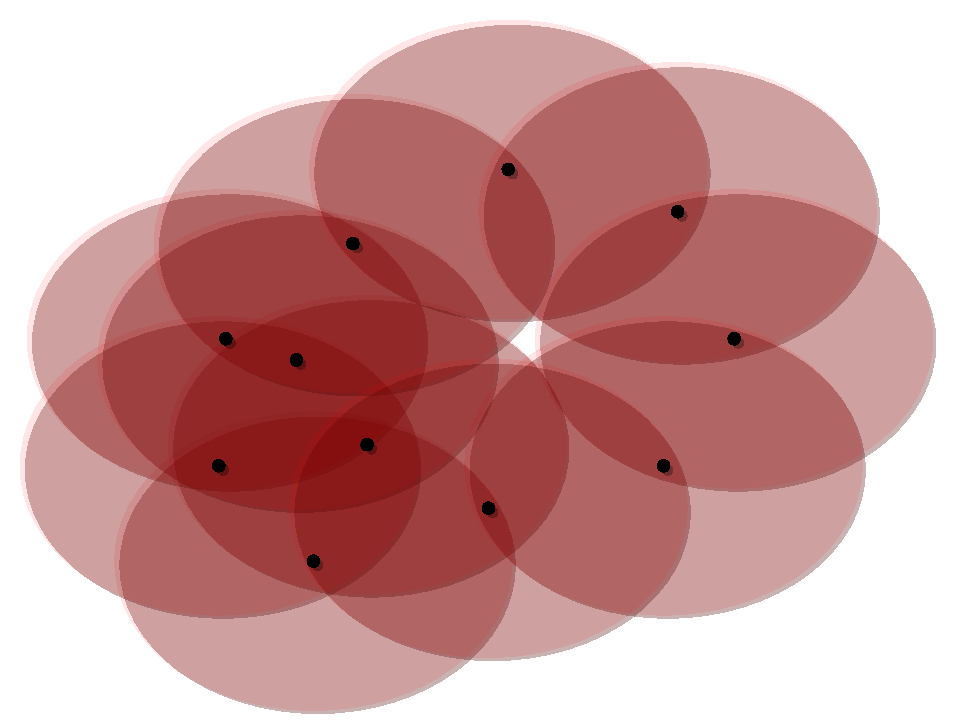
\includegraphics[scale=0.33]{figures/holes_cover.pdf}
    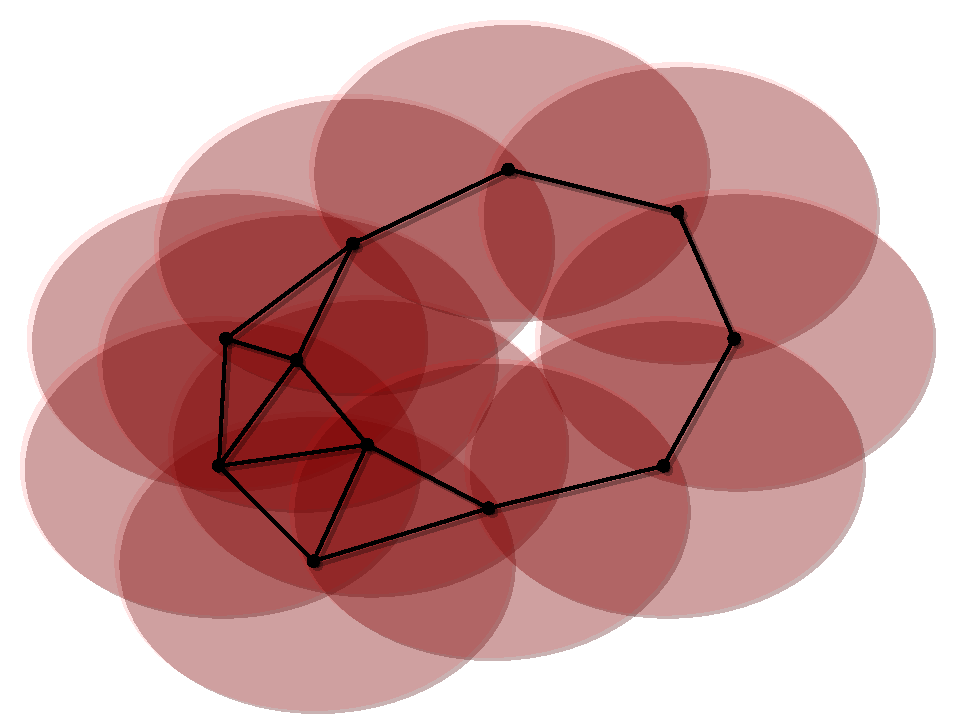
\includegraphics[scale=0.33]{figures/holes_edges.pdf}
    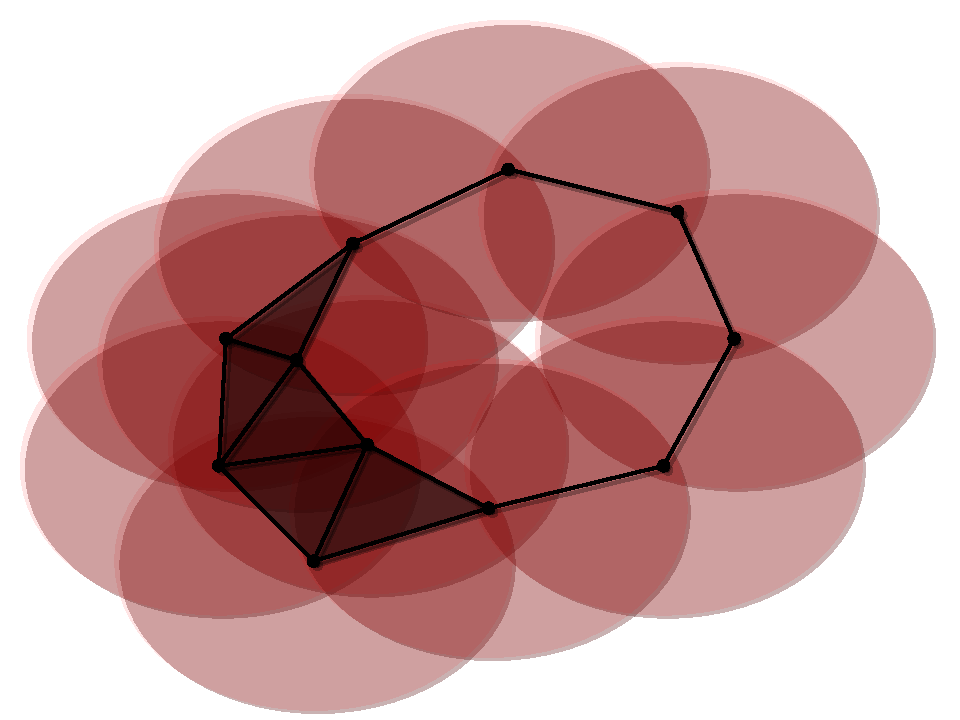
\includegraphics[scale=0.33]{figures/holes_complex.pdf}
     \caption{(Left) The coverage regions of a collection of points $P$ at some scale $\alpha$.
            (Middle) The neighborhood graph with edges for each pair of points within pairwise distance $\alpha$.
            (Right) If we attempt to fill cycles in the graph with triangles identify a cycle that cannot be filled which reflects a gap in coverage}
     \label{fig:holes}
\end{figure}}

It is natural to think of a $k$-dimensional simplicial complex as the generalization of an undirected graph consisting of vertices and edges, collections of at most 2 vertices, to collections of sets of at most $k-1$ vertices.
Just as we have defined a hole in our graph $G$ as a cycle that cannot be filled with triangles, we define a $k$-dimensinal hole in a simplicial complex as a $k$-cycle that cannot be filled with $(k+1)$-simplices.
In the next section we will formally define $k$-cycles and introduce simplicial homology as a tool for identifying when and which cycles cannot be filled.

\paragraph{Coordinate-free Communication}
In a coordinate-free sensor network each sensor, represented by a point in $P$, is capable of detecting nodes which are sufficiently ``close.''
That is, there is some radius of communication $\delta > 0$ such that two nodes $p, q\in P$ such that $\dist(p, q) \leq\delta$ are capable of communication.
Note that, although sensors can communicate within this distance they are not able to measure the distance itself.

With this limited capability we can construct an undirected graph $G=(V, E)$ with vertices $V=P$ and edges $E = \{\{p, q\}\subset P\mid \dist(p,q)\leq\delta\}$.
Let $K$ be a simplicial complex with 0-simplices $\{v\}$ for all $p\in P$, 1-simpices $\{u, v\}\subset P$ for each edge in $E$, and 2-simplices $\{u,v,w\}\subset P$ whenever $\{\{\{u,v\},\{v,w\},\{u,w\}\}\subset E$.
This particular simplicial complex is known as the Vietoris-Rips complex.
It is also an example of a clique complex, where the simplices are the complete subgraphs (or cliques) in a given graph.
\begin{definition}
    The \textbf{(Vietoris-)Rips complex} is defined for a set $P$ at scale $\e > 0$ as
    \[ \rips_\e(P) = \left\{\sigma \subseteq P\mid \forall p,q\in\sigma,\ \dist(p, q)\leq \e\right\}. \]
\end{definition}

\paragraph{Coverage}
% In order to determine coverage we must at least assert that the coverage domain spanned by the points in $P$ does not contain any holes.
% Assuming the coverage radius of our sensors is equal to their communication radius $\delta$ we may define a hole in coverage as a cycle that cannot be ``filled'' with triangles (see Fig.~\ref{fig:holes}).

\figblock{%
\begin{figure}[htbp]
\centering
    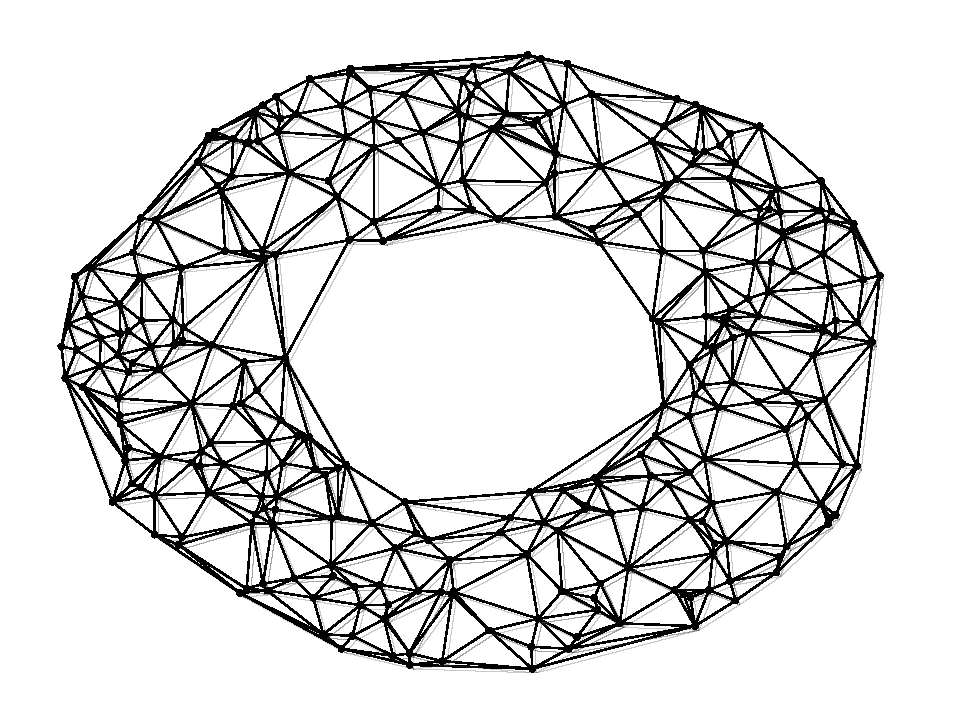
\includegraphics[scale=0.33]{figures/boundary_graph.pdf}
    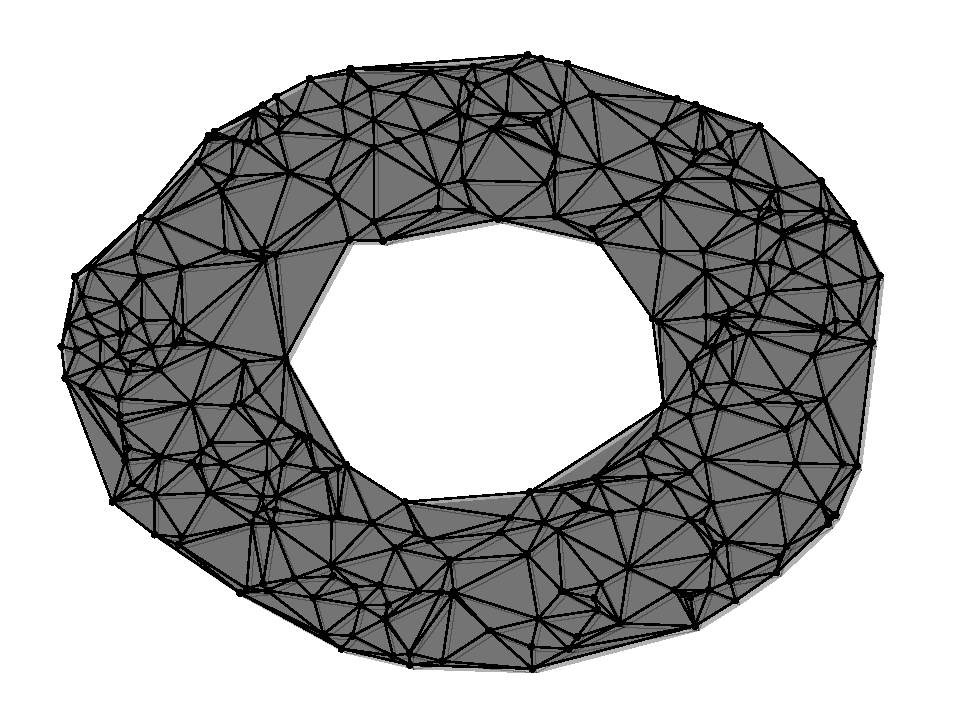
\includegraphics[scale=0.33]{figures/boundary_complex.pdf}
    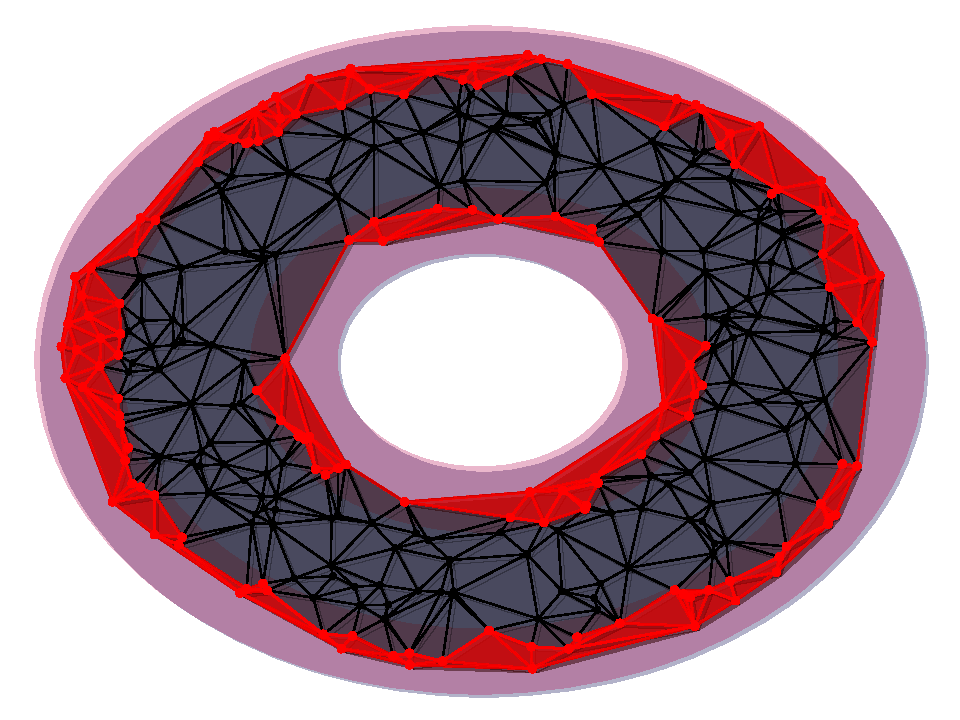
\includegraphics[scale=0.33]{figures/boundary_complex_domain_fence.pdf}
    % 
\includegraphics[scale=0.24]{figures/boundary_domain.pdf}
     \caption{(Left) The neighborhood graph of a sensor network with a large ``hole''.
            (Middle) A 2-dimensional simplicial complex with no gaps in coverage, but an unfilled cycle.
            (Right) By allowing nodes to identify the boundary (in red) we can confirm coverage of complex domains.}
     \label{fig:boundary1}
 \end{figure}}

If a sensor network $P$ covers a domain at scale $\e$ the topology of the domain is reflected in $\rips_\e(P)$.
However, as we will see, this does not necessarily give a tight bound on the minimum radius for coverage.
In fact, if the coverage region of of a sensor network at scale $\alpha$ has no gaps, then the minimum coverage radius required is a constant factor smaller than $\alpha$.
This point is made clear by an interleaving of the Rips with another simplicial complex known as the \v Cech complex.

\begin{definition}
    The \textbf{\v Cech complex} of a finite collection of points $P$ at scale $\e > 0$ is defined
    \[ \cech_\e(P) = \left\{\sigma \subseteq P\mid \bigcap_{p\in \sigma}\ball_\e(p)\neq \emptyset \right\}. \]
\end{definition}
The \v Cech complex is a special case of a more general construction known as the \textbf{nerve} $\N(\U)$ of a collection of sets $\U = \{U_i\}_{i\in I}$, where $I$ is any indexing set.
The nerve of $\U$ is defined as the simplicial complex with vertex set $I$ such that $\sigma\subseteq I$ is a simplex if and only if
\[
  \bigcap_{i\in \sigma} U_i\neq \emptyset.
\]
The collection $\U$ is a \textbf{good cover} if for each $\sigma\subset I$ the set $\bigcap_{i\in\sigma} U_i$ is contractible or empty.
The \textbf{Nerve Lemma} states that if $\U$ is a good cover then its nerve $\N(\U)$ is homotopy equivalent to $\bigcup_{i\in I} U_i$.
That is, for a set of nodes $P\subset\D$ such that $\U = \{\ball_\e(p)\mid p\in P\}$ is a good cover the nerve $\N(\U)$ is homotopy equivalent to $P^\e = \bigcup_{p\in P} \ball_\e(p)$.
It follows that the \v Cech complex $\cech_\e(P)$ of $P$ at scale $\e$ is a suitable representation of the coverage region $P^\e$.

\paragraph{Coordinate-free Coverage}
We will assume that the coverage radius of our sensor network is equal to the radius of communication.
In order to construct the \v Cech complex our sensors must be able to measure not only the proximity of neighboring nodes, but the precise distance between them.
Fortunately, the \v Cech and Rips complexes of a finite metric space are closely related by a result that follows from Jung's Theorem~\cite{jung01uber} relating the diameter of a point set $P$ and the radius of the minimum enclosing ball:
\[\cech_{\e/\jungd}(P)\subseteq\rips_\e(P)\subseteq\cech_\e(P)\subseteq\rips_{\jungd\e}(P),\]
where the constant $\jungd = \sqrt{\frac{2d}{d+1}}$ (see~\cite{buchet15efficient}).

Equipped with this interleaving we are now ready to define all conditions necessary for verifying coverage in a coordinate-free sensor network.
Specifically, we will introduce a second radius of communication $\gamma\geq 3\alpha$ that will allow us to lower $\gamma$, which will remain our coverage radius, so that homomorphism on (relative) homology induced by the inclusion of Rips complexes $\rips_\delta(P)\to\rips_\gamma(P)$ reflects that of the \v Cech complex, and therefore the coverage domain.

% In order to \textit{verify} coverage by we need our network to sufficiently sample the extent of our domain.
% Moreover, if there are gaps in coverage, we would like to know if they are due to insufficient sampling or to a gap in the domain itself.
% Let $\B\subset\D$ be the \textbf{boundary} of our domain and let our sensors detect when they are within the communication radius of $\B$.
% Let $Q = \{p\in P\mid \min_{x\in\B}\dist(x, p)\}$ be the set of \textbf{boundary nodes} in $P$.
% The set $Q$ induces a \textbf{subcomplex} $\rips_\alpha(Q)$ of $\rips_\alpha(K)$ restricted to nodes in $Q$.
% % Assuming there are no holes in our network no path from a point in $P\setminus Q$ to a point outside our domain  without crossing a simplex in $K\mid_Q$.
%
% % \textbf{TODO} Section overview.
% % We will show how this construction is used to verify coverage of a specific subset of a bounded domain $\D$ with a tight bound on the coverage radius.
%
% % Note that the communication radius is far from a tight bound on the coverage radius.

% Throughout we have been using the Rips complex as a discrete representation of our coverage domain by assuming the sensor coverage radius is equal to the communication radius.

% section complexes (end)

  % !TeX root = main.tex

\subsection{Homology} % (fold)
\label{sec:homology}

Simplicial complexes not only provide a comprehensive discretization of continuous domains, but are the primary tool for concrete calculations in algebratic topology.
In particular, the study of simplicial homology groups rely on simplicial complexes in order to study important topological invariants of a discretized space.

The following vector spaces may be defined over any field $\F$, however we will assume the field $\F_2$ in order to avoid orienting the simplices in $K$.
Let $C_k(K)$ denote the vector space over some field $\F$ consisting of linear combinations of $k$-simplices in $K$, which form a basis for $C_k(K)$, known as \textbf{$k$-chains}.
These vector spaces are connected by \textbf{boundary maps} $\partial_k:C_k(K)\to C_{k-1}(K)$ which are linear transformations taking basis elements of $C_k(K)$ to the abstract sum of basis $(k-1)$-simplex faces.
The collection of chains and boundary maps forms a sequence of vector spaces known as the \textbf{chain complex} $\C = (C_*,\partial_*)$
\[
    \ldots\xrightarrow{\partial_{k+1}}
    C_k(K)\xrightarrow{\partial_{k}}
    C_{k-1}(K)\xrightarrow{\partial_{k-1}}
    \ldots\xrightarrow{\partial_2}
    C_1(K)\xrightarrow{\partial_{1}}
    C_0(K)\xrightarrow{\partial_0} 0.
\]

An important property of the boundary maps $\partial_k$ is that the composition of subsequent boundary maps is zero.
That is, for all $k$
\[
  \partial_k\circ\partial_{k-1} = 0.
\]
As a result the image of $\partial_{k+1}$, denoted $\im\partial_{k+1} = \{\partial_{k+1}c\mid c\in C_{k+1}(K)$ is a subspace of the kernel, $\ker\partial_k = \{c\in C_k(K)\mid \partial_k c = 0\}$, of $\partial_k$.
A \textbf{$k$-cycle} of $\C$ is a $k$-chain with empty boundary---an element of $\ker\partial_k$.
Two cycles in $\ker\partial_k$ are said to be \textbf{homologous} if they differ by an element of $\im\partial_{k+1}$.
This leads us to the definition of the homology groups of $K$ as quotient vector spaces $H_k(K)$ over $\F$.

\begin{definition}
    For $k\in\N$ the \textbf{$k$th homology group} of a simplicial complex $K$ is the quotient group
    \[ \hom_k(K) = \ker\partial_k/\im~\partial_{k+1}. \]
\end{definition}

The rank of a homology group is of particular importance and is known as the \textbf{Betti number} $\beta_k = \rank~ \hom_k(K)$.
These topological invariants can be thought of as counting the number of $k$-dimensional ``holes'' in a topological space, where $0$-dimensional holes are connected components, $1$-dimensional holes are loops, $2$-dimensional holes are voids, and so on.
Note that this is the same notion which motivated our use of simplicial complexes for determining coverage---a $1$-dimensional hole exists if a gap in a neighborhood graph cannot be filled by triangles.

\paragraph*{\textbf{Relative Homology}}

\figblock{%
\begin{figure}[htbp]
\centering
    
\includegraphics[scale=0.5]{figures/balloons1.png}\vspace{2ex}
    
\includegraphics[scale=0.5]{figures/balloons3.png}
    \caption{(Left) Two connected, planar domains with boundaries (in red).
            We can gather some intuition for the relative homology of a pair $(\D,\B)$ by thinking about wrapping the interior of the domain around its boundary, and identifying all points in the boundary with a point (Right).
            Even with disconnected boundaries we know that $\beta_2 = \rank~ H_2(\D, \B) = 1$.  That is, there is just one enclosed void.}
    \label{fig:balloons1}
\end{figure}}

For a simplicial complex $K$ let $L\subset K$ be a subcomplex of $K$.
Let $\C(K, L)$ denote the quotient chain complex of pairs $(C_k(K, L), \overline{\partial_k})$ where $C_k(K, L) = C_k(K)/C_k(L)$ consists of the chains on $K$ modulo chains on $L$, with the induced boundary maps $\overline{\partial_k}$ on the quotients.
Each relative chain is an equivalence class of chains in $K$ which are identical without the elements of $L$.
The \textbf{relative homology groups} $\hom_k(K, L)$ consist of homology classes of relative cycles---chains in $K$ whose boundaries vanish or lie in $L$.
That is, a relative cycle can either be a cycle in $K$ or a chain in $K$ with a boundary in $L$.

\begin{theorem}[Excision]\label{thm:excision}
    Let $X$ be a topological space and $A$ and $U$ be subspaces such that $U$ is also a subspace of $A$.
    If $\cl(U)\subseteq \intr(A)$ then $\hom_*(X\setminus U, A\setminus U)\cong \hom_*(X, A)$.
\end{theorem}

\begin{corollary}
    If $\intr(A)\cup \intr(B) = X$ then $\hom_*(X, A)\cong \hom_*(B, A\cap B)$.
\end{corollary}

% section homology (end)

  % !TeX root = main.tex

\subsection{Persistent Homology}

\paragraph*{\textbf{Functions and Filtrations}}

\figblock{%
\begin{figure}[htbp]
\centering
    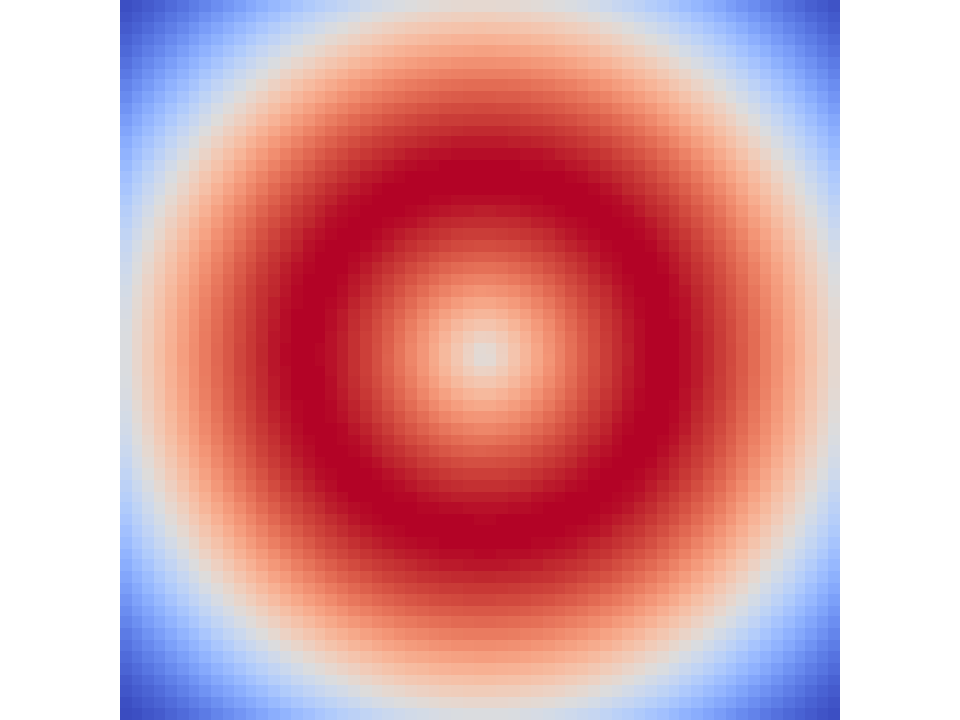
\includegraphics[scale=0.45]{figures/fgrid.pdf}
    % 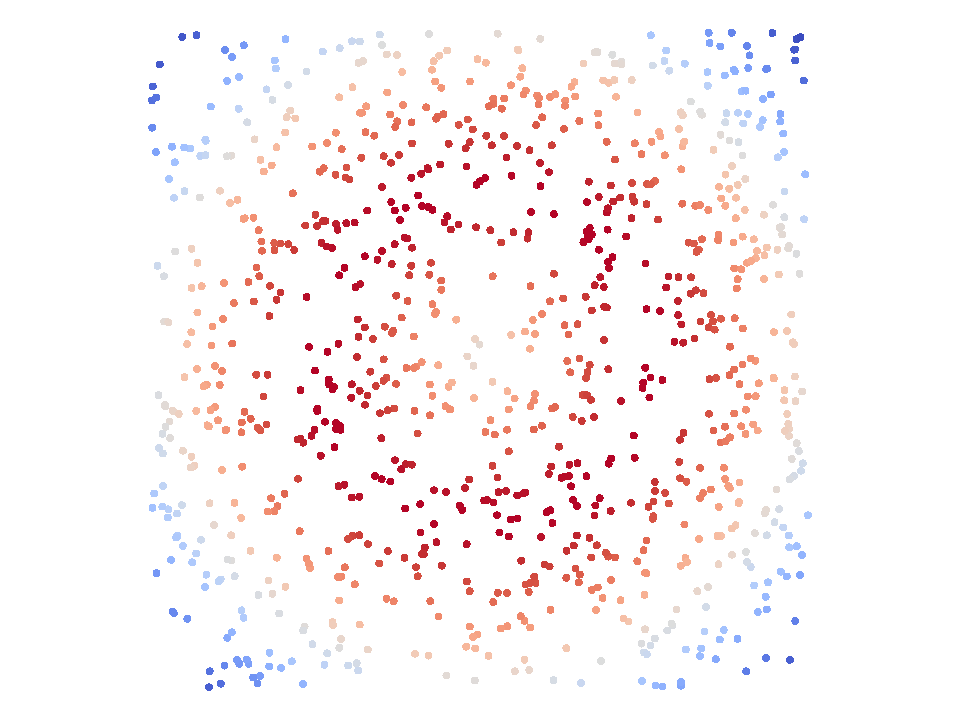
\includegraphics[scale=0.45]{figures/fsample.pdf}
    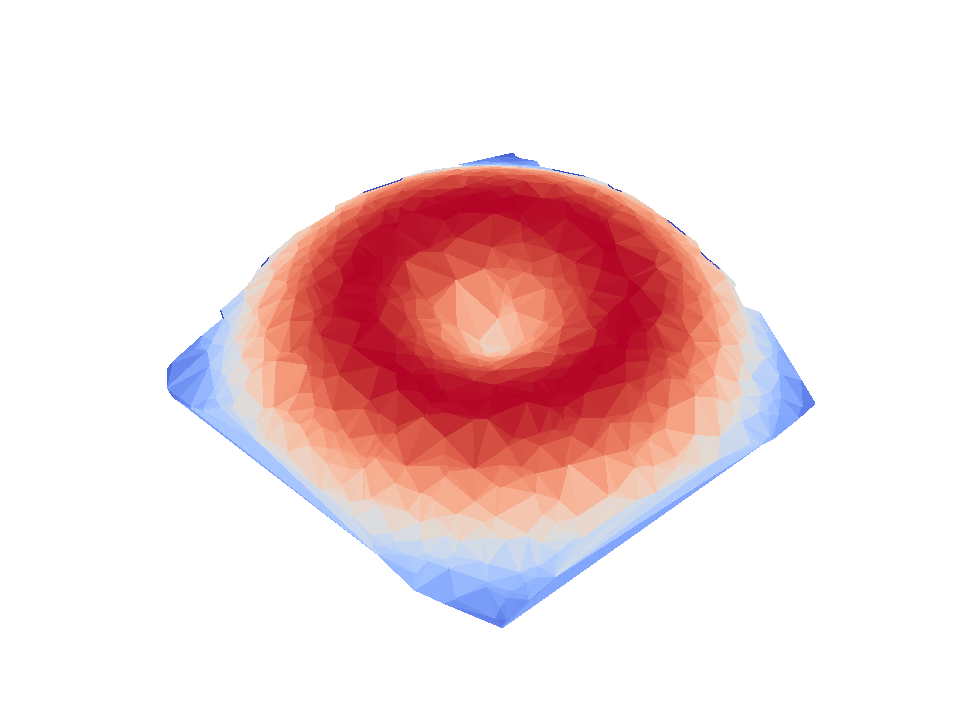
\includegraphics[scale=0.55]{figures/fcomplex.pdf}
    \caption{(Left) Continuous function on the plane.
            % (Middle) Function values on random sample.
            (Right) Function values on a random sample extended to a continuous piecewise linear approximation on a 2-dimension simplicial as the $z$-axis.}
    \label{fig:function}
\end{figure}}

Suppose we have some real valued function $f:\D\to\R$ and endow our sensors with the ability to measure this function at their points $P$.
If we know our network covers the domain we may construct a simplicial complex which captures its topology in a discrete structure.
We may therefore integrate the sparse measurements provided by the sensors throughout the simplicial complex to capture the topology of the function itself.
Not only do we now have a discrete approximation of the function but an ordering on the simplices of the complex which may be used to explore the evolution of the topological structure of the function.

This leads to a more general notion defined for a sequence of topological spaces, which we may take as sublevel sets of the function on the domain.
\begin{definition}
    Let $f:\D\to\R$ be a function on a topological domain $\D$ and let $I_0, I_1,\ldots$ be a sequence of intervals $I_i = [a_i, b_i)$ that covers the image of $f$ on $\D$.
    Let and $X_i = \{x\in\D\mid a_i\leq f(x) < b_i\}$ be topological subspaces connected by inclusion maps $X_i\to X_{i+1}$.
    A \textbf{filtration} is the resulting sequence of topological spaces
    \[X_0\to X_1\to\ldots X_i\to X_{i+1}\to\ldots .\]
\end{definition}
A filtration $\{K_i\}_{i=1,\ldots,n}$ may also be interpreted as a sequence of simplicial maps, each an inclusion $K_i\to K_{i+1}$.
This induces an algebraic sequence of homomorphisms on homology by functoriality, for all $k$:
\[ H_k(X_0)\to H_k(X_1)\to\ldots\to H_k(X_i)\to H_k(X_{i+1})\to\ldots . \]
This sequence encodes the local topological changes that occur at each step of the filtration.
Global information is encoded in terms of the \textbf{birth} and \textbf{death} of homology classes, represented as a \textbf{persistence diagram} or \textbf{barcode}.

% \vspace{0.25in}
% \textbf{TODO} Persistence diagram of a function on a simplicial complex
% \vspace{0.25in}

% \figblock{%
% \begin{figure}[htbp]
% \centering
%     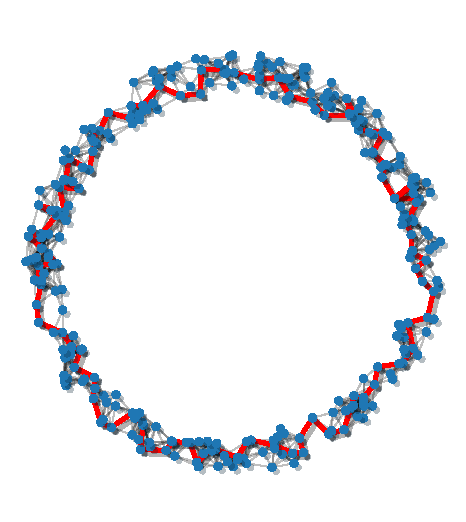
\includegraphics[scale=0.9]{figures/homology_cycle.pdf}\hspace{10ex}
%     % 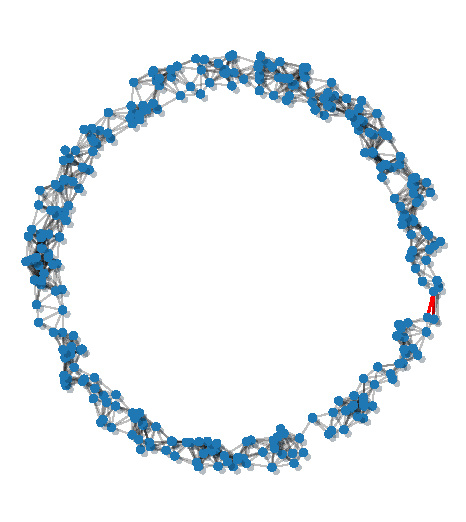
\includegraphics[scale=0.6]{figures/cohomology_cocycle.pdf}
%     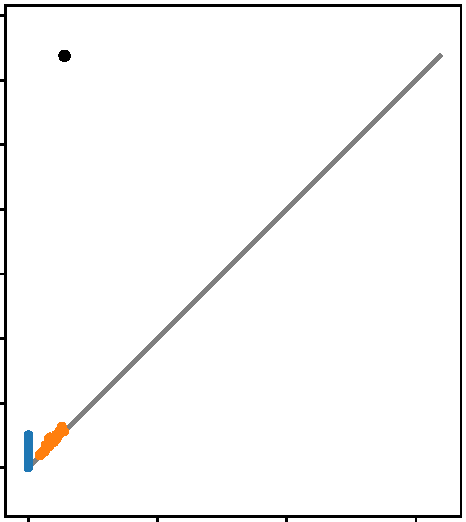
\includegraphics[scale=0.8]{figures/homology_dgm.pdf}
%     \caption{The representative cycle of a significant feature in the persistent homology of rips filtration of a noisy circle.
%             The birth of the feature indicated on the persistence diagram (right) corresponds to the scale of the rips complex shown (left) when the circle, a 1-cycle, is born.
%             The death of this feature corresponds to the scale of the rips complex at a larger scale (not shown) when a triangle first fills the interior of the circle.
%             This scale is approximately the length of the edges in the smallest equilateral triangle with sample points as vertices that contains the centroid of the sample.
%             This illustrates the geometric information encoded in the persistence diagram of geometric complexes as it is within a constant factor of the radius of the circle.}
%     \label{fig:cycle_diagrams}
% \end{figure}}
%
% Given a simplicial complex $K$ on a set of points $P\subset\D$ and a function $f:\D\to\R$ we may construct a filtration $\{K_i\}_{i=1,2,\ldots}$ by ordering the simplices by their function values.
% For example, $f(\sigma) = \max_{v\in\sigma} f(v)$ for any simplex $\sigma\in K$.
% The resulting filtration is now a sequence of simplicial maps, each an inclusion $K_i\to K_{i+1}$, which induces a sequence of homology groups.

% \subsection{Persistent Homology}
%
% \begin{figure}[htbp]
% \centering
%     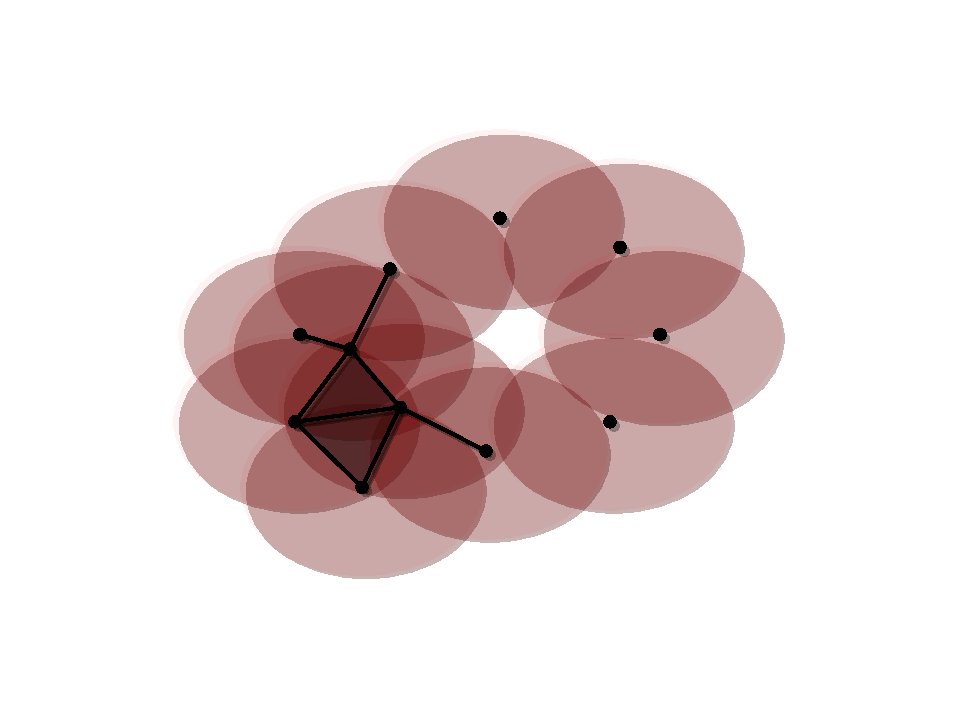
\includegraphics[scale=0.4]{figures/persist06.pdf}
%     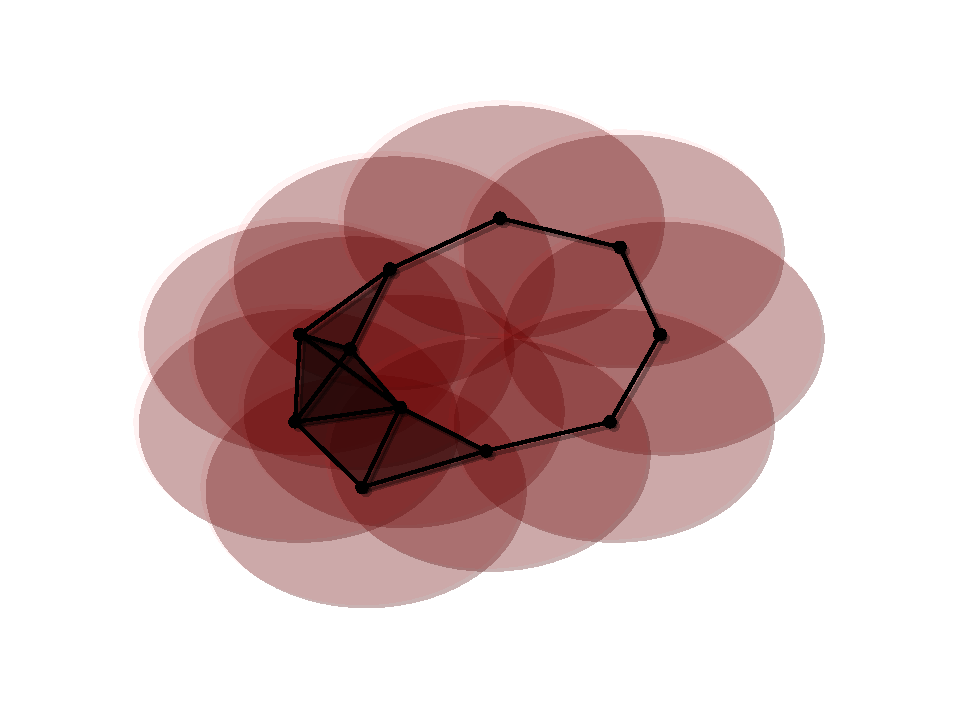
\includegraphics[scale=0.4]{figures/persist08.pdf}
%     % 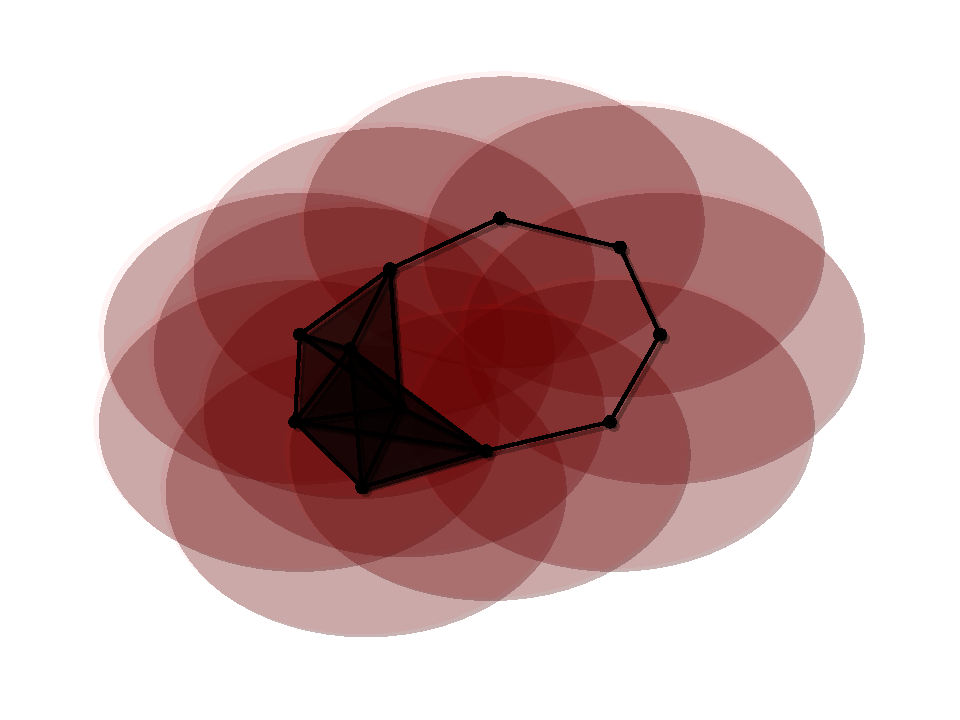
\includegraphics[scale=0.4]{figures/persist10.pdf}
%     % 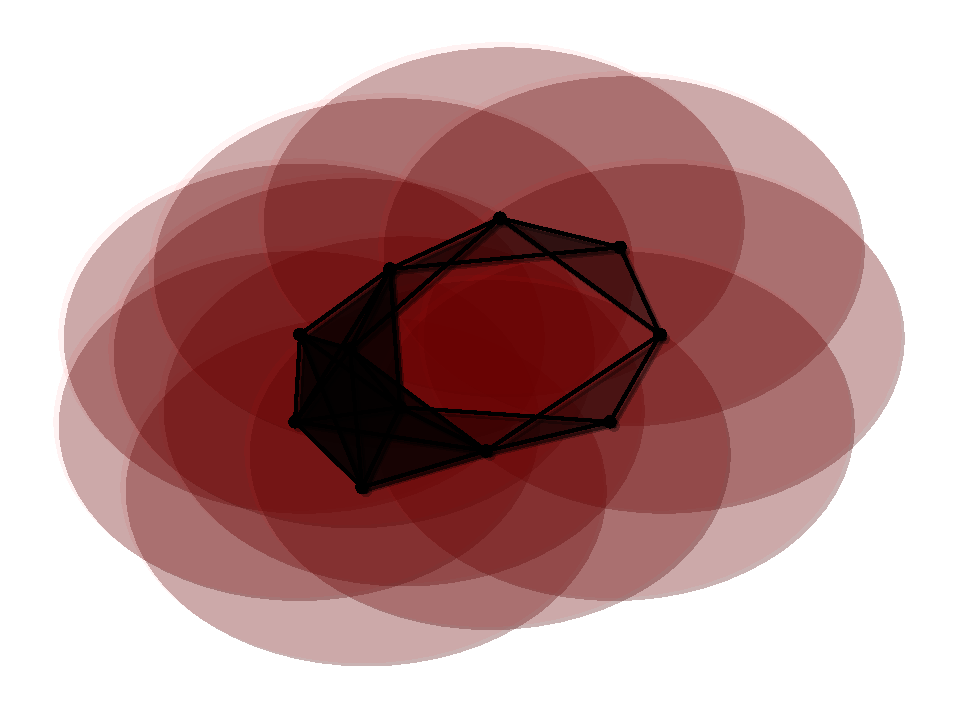
\includegraphics[scale=0.4]{figures/persist12.pdf}
%     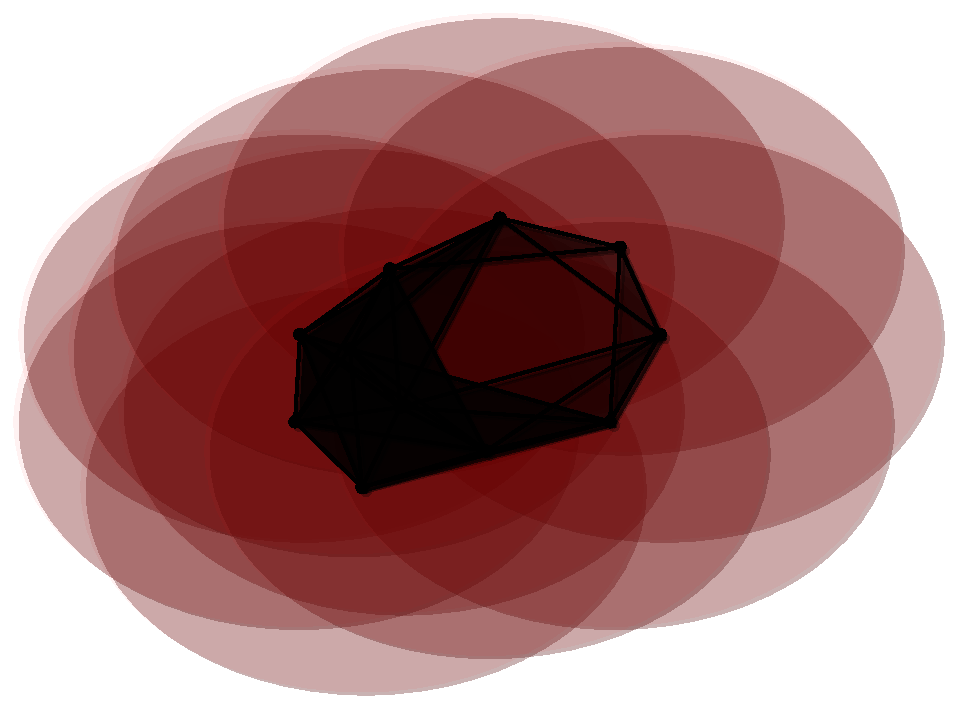
\includegraphics[scale=0.4]{figures/persist14.pdf}
%     \caption{A filtration of rips complexes at scales 0.6, 0.8, and 1.4 illustrating a point $(0.8, 1.4)$ in the corresponding persistence diagram. The 1-cycle that is born at scale 0.8 persists until it dies at scale 1.4.}
%     \label{fig:persist}
% \end{figure}
%
% % \vspace{0.25in}
% % \textbf{TODO} ``Metric'' persistence.
% % \vspace{0.25in}
%
% % Topological data analysis is an emerging field in the intersection of data analysis and algebraic topology which extends the notion of homology and cohomology groups to a more analytical tool known as \textbf{topological persistence}.
% % Where simplicial homology identifies invariants of a static simplicial complex persistent homology tracks the evolution of a sequence of nested simplicial complexes which provide a more detailed topological signature, in addition to relevant geometric information.
%
% Just as we can construct a filtration from a function on a simplicial complex we can construct a filtration from the metric induced on our sample by the domain.
% Let $P$ be a finite metric space with $m$ points and let $K = \rips_\alpha(P)$ be the Rips complex of $P$ at scale $\alpha$ consisting of $n$ simplices.
% We can order the simplices $\sigma_1,\ldots,\sigma_n$ by the minimum pairwise distance between their vertices by first applying an arbitrary ordering on the vertices $v_1,\ldots,v_m$ and letting $\sigma_i = \{v_i\}$ for $i=1,\ldots,m$ so that $K_i = \{\sigma_1,\ldots, \sigma_m\}$.
% We can then build a filtration $\K = \{K_i\}_{i=1,\ldots,n}$ so that $K_i = \rips_\e(P)$ where $\e = \max_{u,v\in\sigma_i}\dist(u,v)$ by adding one simplex at a time, breaking ties first by dimension, then by the ordering on their constituent vertices.
% A $k$-dimensional feature is identified when a $(k+1)$-simplex $\sigma$ is added that kills a $k$-cycle $\gamma$.
% In the persistence diagram, this feature would be represented by a point $(b, d)$ where $b$ is the smallest scale for which the $k$-cycle appears
% \[ \tau\in\rips_b(P)\text{ for all }\tau\in\gamma\]
% and $d = \max_{u,v\in\sigma}\dist(u,v)$ is the scale at which $\sigma$ enters the filtration.
% The result is a collection of points $(b_i, d_i)$ in the plane for each dimension $k$ known as the persistence diagram, denoted $\dgm_k(\K)$.
% A persistence diagram is depicted on the right in Fig.~\ref{fig:cycle_diagrams}.

\paragraph*{\textbf{Persistent Homology.}} % (fold)
\label{par:persistent_homology}

Given a filtration $\mathcal{F} = \{F_\alpha\}_{\alpha\in\R}$ the inclusions $F_\alpha\hookrightarrow F_\beta$ induce homeomorphisms between homology groups $h_*^{\alpha,\beta} : H_*(F_\alpha)\to H_*(F_\beta)$.
The \emph{persistent homology modules} of $\F$ are the pairs
\[\mathcal{H}_*(\F) = (\{H_*(F_\alpha)\}_{\alpha\in\R}, \{h_*^{\alpha,\beta}\}_{\alpha\leq\beta\in\R}).\]

The persistent homology modules of a filtration $\F$ are each given by a signature known as a \emph{persistence diagram}, denoted $\Pers_*(\F)$, where $\Pers(\F)$ is used to refer to the collection of persistence diagrams of all dimensions.
Unless otherwise noted we will refer $\Pers(\F)$ as the persistence diagram of $\F$.

The space of persistence diagrams is a metric space $(\PPers, \dist_B)$ under the \emph{bottleneck distance} which is defined for diagrams $A, B$, taken as multisets in $\R^2$ equipped with the $l^\infty$-norm, as
\[\dist_B(A, B) = \min_{\gamma:A\to B}\max_{p\in A} \| p- \gamma(p)\|_\infty\]
where $\gamma$ ranges over all bijections from $A$ to $B$.

\paragraph*{\textbf{Stability of Persistent Homology.}} % (fold)
\label{par:stability_of_persistent}

The persistent homology of Rips filtrations constructed from point clouds in euclidean space is closely related to the sequence of metric balls growing around the point cloud as the persistent homology of both gives a signature for distance to the point cloud.
In particular, the persistent homology of the Rips complex of a point cloud approximates that of the distance to the point cloud as a function on the underlying metric space.

\figblock{%
\begin{figure}[htbp]
\centering
    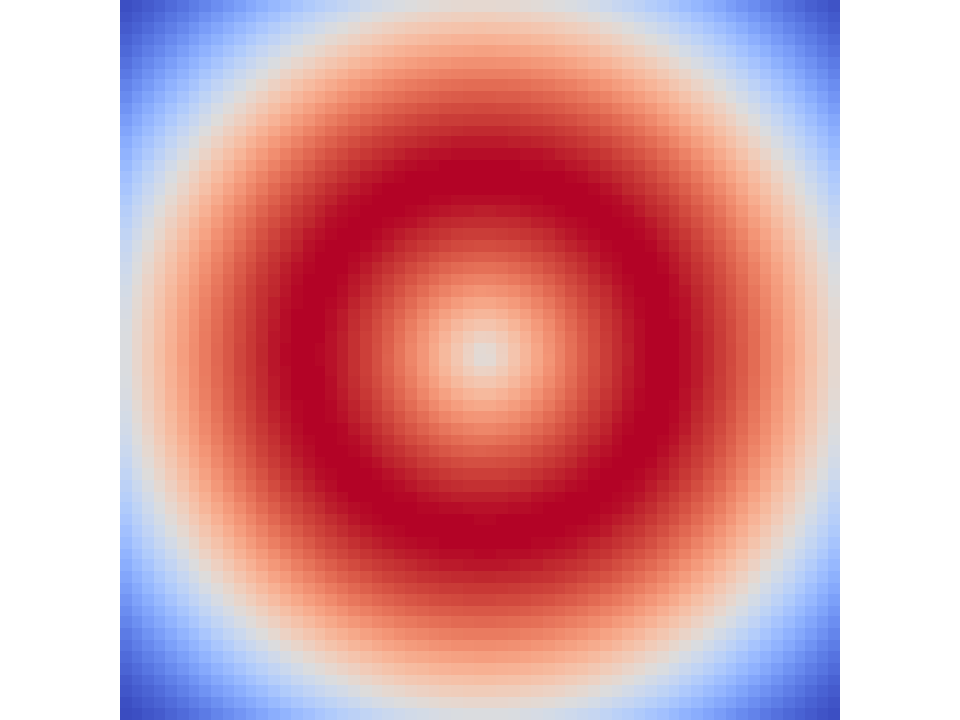
\includegraphics[width=0.29\textwidth,trim={0 -1.5cm 0 0},clip]{figures/fgrid.pdf}
    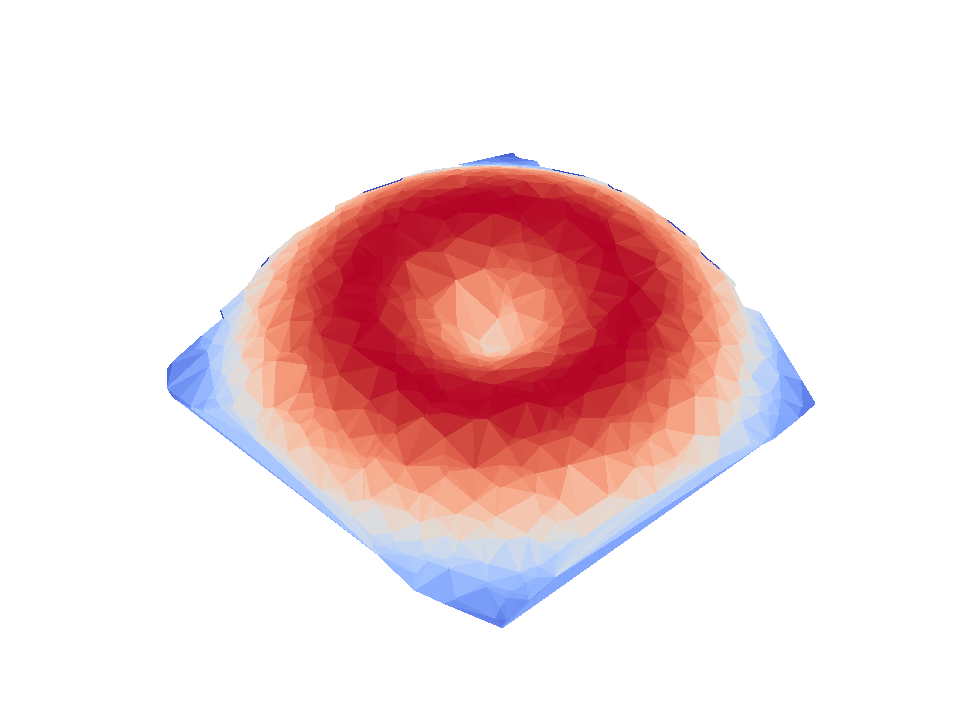
\includegraphics[width=0.4\textwidth]{figures/fcomplex.pdf}
    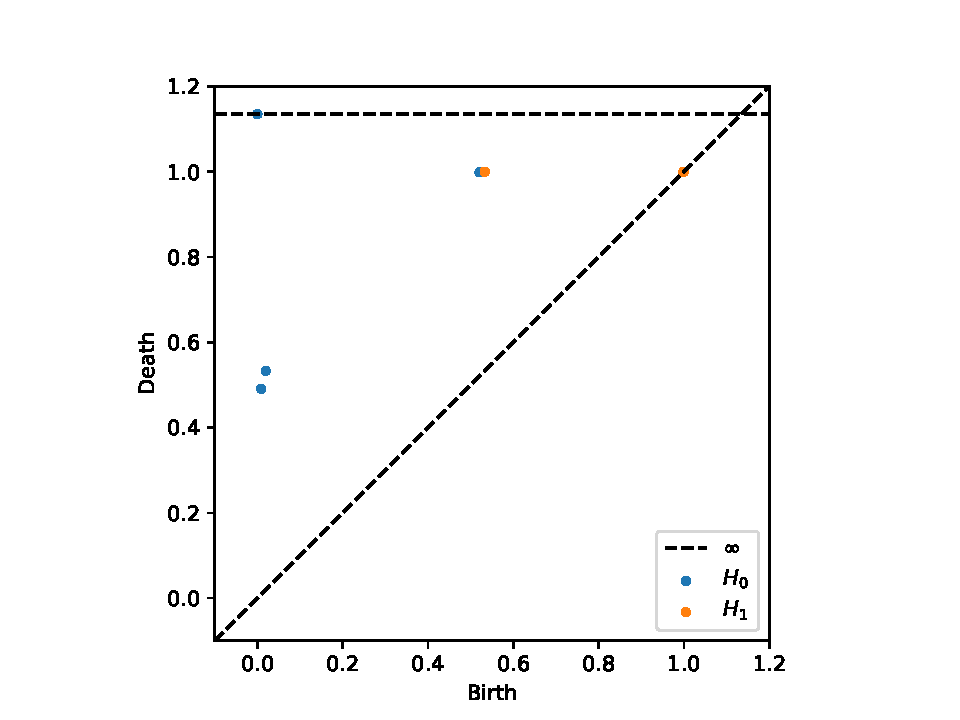
\includegraphics[width=0.29\textwidth,trim={2cm 0cm 2cm 1cm},clip]{figures/fdgm.pdf}
    \caption{(Left) Continuous function on the plane.
            (Middle) Function values (as $z$-axis) on a random sample extended to a simplicial complex.
            (Right) Persistence diagram of an induced filtration.}
    \label{fig:function}
\end{figure}
}

More generally, the persistent homology of a real-valued function captures the changes in the homology groups of its \emph{sublevel-sets}---the set of points with function values below a given scale.
The distance to a point cloud is a real-valued function with sublevel-sets equal to the union of metric balls at a given scale.
Under certain conditions we can approximate the persistent homology of a real-valued function given only its values on a finite subset of its domain.

Given a topological space $X$ and a real-valued function $f:X\to\R$ the \emph{sublevel-set filtration} of $f$ is the sequence $\{X^f_\alpha\}_{\alpha\in\R}$ of sublevel-sets $X^f_\alpha = f^{-1}(-\infty, \alpha]$.
We define a metric $\dmax$ between two real-valued functions $f,g:X\to\R$ by taking the maximum difference of the functions on any point, i.e.
\[ \dmax(f, g) := \max_{x\in X} |f(x) - g(x)|. \]

\begin{lemma}\label{lem:interleave}
    Let $X$ be a topological space and $f,g: X\to\R$ are tame functions such that $\dmax(f, g)\leq\e$.
    Then the sublevel-set filtrations $\{X_\alpha^f\}_{\alpha\in\R}$ of $f$ and $\{X_\alpha^g\}_{\alpha\in\R}$ of $g$ are $\e$-interleaved.
\end{lemma}

The following is a standard result in the stability of persistence diagrams.

\begin{lemma}\label{lem:stability}
    If two filtrations $\F$ and $\F'$ are $\e$-interleaved then
    \[ \dist_B(\Pers(\F), \Pers(\F'))\leq\e. \]
\end{lemma}

The persistent homology modules of the sublevel-set filtration $\{X^f_\alpha\}_{\alpha\in\R}$ are referred to as the persistent homology modules $\mathcal{H}_*(f)$ of $f$ with its diagram denoted $\Pers(f)$.

\begin{corollary}\label{cor:stability}
    If $X$ is a topological space and $f,g:X\to\R$ are tame functions then
    \[ \dist_B(\Pers(f), \Pers(g))\leq\dmax(f, g). \]
\end{corollary}

  % % !TeX root = main.tex

% \section{Background}
% \label{sec:background}

% \paragraph*{\textbf{Simplicial Complexes.}}
%
% A \textbf{simplicial complex} $K$ with vertex set $V$ is a collection of \textbf{simplices} $\sigma\subset V$ that is closed under taking subsets.
% We define a \textbf{pair of complexes} to be a pair $(K, L)$ where $K$ is a simplicial complex and $L$ is a subcomplex of $K$.
%
% Given a metric space $(X, d)$ we define the $\e$-offsets of a point $p\in X$ as \[\ball(p, \e) = \{x\in X\mid d(x, p)\leq \e\}.\]
% For a subset $P\subseteq X$ the \emph{nerve} of a family $\{\ball(p,\e)\}_{p\in P}$ is the abstract simplicial complex with vertex set $P$ with simplices corresponding to subsets of elements with nonempty intersections, and is known as the \emph{\v{C}ech complex}
% \[
%   \cech_\e(P) := \left\{\sigma \subseteq P\mid \bigcap_{p\in \sigma}\ball(p,\e)\neq \emptyset \right\}.
% \]
% The \textbf{(Vietoris-)Rips complex} of $P$ at scale $\e$ is defined as
% \[
%   \rips_\e(P) := \left\{\sigma \subseteq P \mid \{p,q\}\in\cech_\e(P) \text{ for all $p,q\in \sigma$}\right\}.
% \]
%
% For any metric space $(X, d)$ the \v{C}ech and Rips complexes of a subset $P\subset X$ are related by the following interleaving for all $\e > 0$
% \[ \cech_{\e/2}(P)\subseteq \rips_\e(P)\subseteq \cech_\e(P). \]
%
% \paragraph*{\textbf{Homology and Persistent Homology.}} % (fold)
% \label{par:homology_and_persistent_homology}
%
% Homology is a tool from algebraic topology that provides a topological signature for a shape that may be readily computed from a matrix representation of a finite simplicial complex through matrix reduction.
% The resulting signature is invariant under homeomorphisms and homotopy equivalences, and may be thought of as quantifying the components, loops, and voids in a topological space.
%
% Throughout, we assume singular homology over a field, where the \emph{$k$th homology group} of a space $X$ is a vector space denoted $H_k(X)$.
% We will write $H_*(X)$ to denote the homology of all dimensions.
% For a pair of spaces $(X,Y)$ with $Y\subseteq X$ the \emph{relative homology groups} gives the homology of $X$ relative to $Y$, and are denoted $H_*(X,Y)$.
%
% A \emph{filtration} is a sequence of topological spaces $\mathcal{F} = \{F_\alpha\}_{\alpha\in\R}$ that are nested by inclusions $F_\alpha\hookrightarrow F_\beta$ for $\alpha\leq\beta$.
% Each inclusion $F_\alpha\hookrightarrow F_\beta$ induces homeomorphisms between homology groups $h_*^{\alpha,\beta} : H_*(F_\alpha)\to H_*(F_\beta)$.

\paragraph*{\textbf{Analysis of Scalar Fields.}} % (fold)
\label{par:stability_of_persistent}

Figure~\ref{fig:function} depicts a function on a subset of the plane and its function values on the simplices of a simplicial complex defined on a subset of the plane.
The filtration given by ordering the simplices of this complex by their function values is known as an \emph{induced filtration}.
Chazal et. al. detail how to construct a filtration (in fact, the inclusion of two filtrations) that approximates the persistence diagram of the function itself~\cite{chazal09analysis} that has a natural application to measurements by coordinate-free sensor networks.
Extending our testbed to explore this result was a natural next step as it assumes coverage and the structures required are a subset of those used in the computation of the TCC.
This extension has led to promising results on applications to functions on coordinate-free networks over time as well as interesting theoretical questions on the role of the boundary in these experiments.

For a compact Riemannian manifold $X$, possibly with boundary, a point $x\in X$ and a real value $r\geq 0$, let $B_X(x, r) = \{y\in X\mid d_X(x,y) < r\}$ denote the open geodesic ball of center $x$ and radius $r$.
For all sufficiently small values $r\geq 0$ the ball $B_X(x,r)$ is said to be \emph{strongly convex} if for every pair of points $y,y'$ in the closure of $B_X(x, r)$, there exists a unique shortest path in $X$ between $y$ and $y'$, and the interior of this path is included in $B_X(x, r)$.
Let $\varrho(x) > 0$ be supremum of the radii such that this property holds.
The \emph{strong convexity radius} of $X$ is defined $\varrho(X) = \inf_{x\in X}\varrho(x)$.
Because $X$ is compact $\varrho(X)$ is known to be positive.
This quantity is required in order to apply the Nerve theorem in Theorem~\ref{thm:scalar}.
% In the following let $R_\delta^{\delta'}(P) = \im (R_{\delta}(P)\hookrightarrow R_{\delta'}(P))$ denote the image of the inclusion of Rips complexes of some set $P\subseteq X$ at scales $\delta\leq\delta'$.

\begin{theorem}[Theorem 2 of~\cite{chazal09analysis}]\label{thm:scalar}
    Let $X$ be a compact Riemannian manifold, possibly with boundary, and let $f:X\to\R$ be a $c$-Lipschitz function.
    Let also $P$ be a geodesic $\e$-sample of $X$.
    If $\e < \frac{1}{4}\varrho(X)$, then for any $\delta\in [2\e,\frac{1}{2}\varrho(X))$ and for any $k\in\N$, the $k$th persistent homology modules of $f$ and of the nested pair of filtrations $\{\rips_\delta(P_\alpha^f)\hookrightarrow \rips_{2\delta}(P_\alpha^f)\}_{\alpha\in\R}$ are $2c\delta$-interleaved.
    % $\{R_\delta^{2\delta}(P_\alpha^f)\}_{\alpha\in\R}$ are $2c\delta$-interleaved.
    Therefore, the bottleneck distance between their persistence diagrams is at most $2c\delta$.
\end{theorem}

\paragraph*{\textbf{Stability of Relative Persistent Homology.}} % (fold)
\label{par:stability_of_relative_persistent}

Let $(X, Y)$ be a pair of spaces with $Y\subseteq X$.
For $f:X\to\R$ we define a function $\tilde{f}$ on the pair $(X, Y)$ as the pair $(f, f\restriction_Y)$ where $f\restriction_Y:Y\to\R$ is the restriction of $f$ to $Y$.
The \emph{sublevel-set filtration of $\tilde{f}$ on the pair $(X, Y)$} is the sequence of pairs of sublevel-sets $\{(X_\alpha^f, Y_\alpha^f)\}_{\alpha\in\R}$ where $X_\alpha^f = f^{-1}(-\infty,\alpha]$ and $Y_\alpha^f = f\restriction_Y^{-1}(-\infty,\alpha] = X_\alpha^f\cap Y$ are the sublevel-sets of $f$ and $f\restriction_Y$, respectively.

\begin{lemma}\label{lem:relative_interleave}
    Let $X$ be a topological space and $Y\subseteq X$.
    Let $f,g:X\to\R$ be tame functions such that $\dmax(f, g)\leq\e$.
    Then the sublevel-set filtrations $\{(X_\alpha^f, Y_\alpha^f)\}_{\alpha\in\R}$ of $\tilde{f}$ and $\{(X_\alpha^g, Y_\alpha^g)\}_{\alpha\in\R}$ of $\tilde{g}$ on the pair $(X, Y)$ are $\e$-interleaved.
\end{lemma}
\begin{proof}
    By Lemma~\ref{lem:interleave} we have that the sublevel-set filtrations of $f$ and $g$ are $\e$-interleaved.
    Note that, because $Y\subseteq X$, we have that $Y^f_\alpha \subseteq X^f_\alpha$ and $Y^g_\alpha \subseteq X^g_\alpha$ for all $\alpha\in\R$, so the sublevel-set filtrations $\{Y^f_\alpha\}_{\alpha\in\R}$ of $g\restriction_Y$ and $\{Y^g_\alpha\}_{\alpha\in\R}$ of $f\restriction_Y$ are $\e$-interleaved.
    It follows that the sublevel-set filtrations $\{(X^f_\alpha, Y^f_\alpha)\}_{\alpha\in\R}$ of $\tilde{f}$ and $\{(X^g_\alpha, Y^g_\alpha)\}_{\alpha\in\R}$ of $\tilde{g}$ are $\e$-interleaved.
\end{proof}

The \emph{persistent relative homology modules} of a real-valued function $\tilde{f}$ on the pair $(X, Y)$ is a pair consisting of the family of relative homology groups of $\{(X^f_\alpha, Y^f_\alpha)\}_{\alpha\in\R}$ and the connecting homeomorphisms on relative homology groups induced by inclusions of pairs $(X^f_\alpha, Y^f_\alpha)\hookrightarrow (X^f_\beta, Y^f_\beta)$:
\[\mathcal{H}_*(\tilde{f}) = (\{H_*(X^f_\alpha, Y^f_\alpha)\}_{\alpha\in\R}, \{H_*(X^f_\alpha, Y^f_\alpha)\to H_*(X^f_\beta, Y^f_\beta)\}_{\alpha\leq\beta\in\R}).\]
The corresponding \emph{relative persistence diagram} is denoted $\Pers(\tilde{f})$.

\begin{lemma}\label{lem:relative_stability}
    Let $X$ be is a topological space and $Y\subseteq X$.
    If $f,g:X\to\R$ are tame functions such that $\dmax(f, g)\leq\e$ then
    \[ \dist_B(\Pers(\tilde{f}), \Pers(\tilde{g}))\leq\e.\]
\end{lemma}
\begin{proof}
    Because $\dmax(f, g)\leq\e$ the sublevel-set filtrations of $\tilde{f}$ and $\tilde{g}$ on the pair $(X, Y)$ are $\e$-interleaved by Lemma~\ref{lem:relative_interleave}.
    So, by Lemma~\ref{lem:stability}, we have that $\dist_B(\Pers(\tilde{f}), \Pers(\tilde{g}))\leq\e$.
\end{proof}

\begin{corollary}\label{cor:relative_stability}
    If $X$ is a topological space, $Y\subseteq X$, and $f,g: X\to\R$ are tame functions then
    \[ \dist_B(\Pers(\tilde{f}), \Pers(\tilde{g}))\leq \dmax(f, g).\]
\end{corollary}

The following result from~\cite{skraba14approximating} allows us to extend results in absolute persistent homology to relative persistent homology.
Two filtrations $\{A_\alpha\}_{\alpha\in\R}$ and $\{F_\alpha\}_{\alpha\in\R}$ are called \emph{compatible} if for all $\alpha\leq\beta$, the following diagram commutes
\[\begin{tikzcd}
    A_\alpha \arrow[r] \arrow[d] & F_\alpha \arrow[d] \\
    A_\beta \arrow[r] & F_\beta.
\end{tikzcd}\]

\begin{theorem}[Theorem 1 of~\cite{skraba14approximating}]\label{thm:compatible}
    If compatible filtrations $\{F_\alpha\}_{\alpha\in\R}$ and $\{G_\alpha\}_{\alpha\in\R}$ are $\e_1$-interleaved,
    $\{A_\alpha\}_{\alpha\in\R}$ and $\{B_\alpha\}_{\alpha\in\R}$ are $\e_2$-interleaved, then the relative modules $\{(F_\alpha, A_\alpha)\}$ and $\{(G_\alpha, B_\alpha)\}_{\alpha\in\R}$ are $\e$-interleaved, where $\e = \max\{\e_1,\e_2\}$.
\end{theorem}

  % % !TeX root = ../../main.tex

\subsection{Interleaving}

\begin{lemma}%\label{thm:interleaving_main}
  Suppose $\Gamma\in\Hom(\U,\V)$, $\Pi\in\Hom(\V,\W)$, and $\Lambda\in\Hom(\S, \T)$.

  If $\Phi_M(F, G)\in\Hom^\delta(\im~\Gamma, \im~\Lambda)$ and $\Psi_G(M, N)\in\Hom^\delta(\im~\Lambda, \im~\Pi)$ are partial $\delta$-interleavings of image modules such that $\Gamma$ is a epimorphism and $\Pi$ is a monomorphism then $\im~\Lambda$ is $\delta$-interleaved with $\V$.
\end{lemma}
\begin{proof}
  For ease of notation let $\Phi$ denote $\Phi_M(F, G)$ and $\Psi$ denote $\Psi_G(M, N)$.

  If $\Gamma$ is an epimorphism $\gamma_\alpha$ is surjective so $\Gamma_\alpha = V_\alpha$ and $\phi_{\alpha} = g_{\alpha}\rest_{\Gamma_\alpha} = g_\alpha$ for all $\alpha$.
  So $\im~\Gamma = \V$ and $\Phi\in\Hom^\delta(\V,\im~\Lambda)$.

  If $\Pi$ is a monomorphism then $\pi_\alpha$ is injective so we can define a natural isomorphism $\pi_\alpha^{-1} : \Pi_\alpha\to V_\alpha$ for all $\alpha$.
  Let $\Psi^*$ be defined as the family of linear maps $\{\psi_\alpha^* := \pi^{-1}_\alpha \circ \psi_\alpha : \Lambda_\alpha\to V_{\alpha+\delta}\}$.
  Because $\Psi$ is a partial $\delta$-interleaving of image modules, $n_\alpha\circ\lambda_\alpha = \pi_{\alpha+\delta}\circ m_\alpha$.
  So, because $\psi_\alpha = n_\alpha\rest_{\Lambda_\alpha}$ for all $\alpha$,
  \begin{align*}
    \im~\psi_\alpha^* &= \im~\pi^{-1}_{\alpha+\delta}\circ\psi_\alpha\\
                      &= \im~\pi^{-1}\circ (n_\alpha\circ\lambda_\alpha)\\
                      &= \im~\pi^{-1}\circ (\pi_{\alpha+\delta}\circ m_\alpha)\\
                      &= \im~ m_\alpha.
  \end{align*}
  It follows that $\im~v_{\alpha+\delta}^{\beta+\delta}\circ\psi_\alpha^* = \im~v_{\alpha+\delta}^{\beta+\delta}\circ m_\alpha$

  Similarly, because $\Psi$ is a $\delta$-interleaving of image modules $n_\beta\circ t_\alpha^\beta\circ \lambda_\alpha = w_{\alpha+\delta}^{\beta+\delta}\circ\pi_{\alpha+\delta}\circ m_\alpha$.
  Moreover, because $\Pi$ is a homomorphism of persistence modules, $w_{\alpha+\delta}^{\beta+\delta}\circ\pi_{\alpha+\delta} = \pi_{\beta+\delta}\circ v_{\alpha+\delta}^{\beta+\delta}$, so
  \[ n_\beta\circ t_\alpha^\beta\circ \lambda_\alpha = \pi_{\beta+\delta}\circ v_{\alpha+\delta}^{\beta+\delta}\circ m_\alpha.\]
  As $\psi_\beta\circ\lambda_\alpha^\beta = n_\beta\circ\lambda_\alpha^\beta = n_\beta\circ t_\alpha^\beta\rest_{\Lambda_\alpha}$ it follows
  \begin{align*}
    \im~\psi_\beta^*\circ\lambda_\alpha^\beta &= \im~\pi^{-1}_{\beta+\delta}\circ (n_\beta\circ t_\alpha^\beta\circ\lambda_\alpha)\\
      &= \im~\pi^{-1}_{\beta+\delta}\circ (\pi_{\beta+\delta}\circ v_{\alpha+\delta}^{\beta+\delta})\circ m_\alpha\\
      &= \im~v_{\alpha+\delta}^{\beta+\delta}\circ m_\alpha\\
      &= \im~v_{\alpha+\delta}^{\beta+\delta}\circ\psi_\alpha^*.
  \end{align*}
  So we may conclude that $\Psi^*\in\Hom^\delta(\im~\Lambda,\V)$.

  So $\Phi\in\Hom^\delta(\V,\im~\Lambda)$ and $\Psi_G^*\in\Hom^\delta(\im~\Lambda,\V)$.
  As we have shown, $\im~\psi_{\alpha-\delta}^* = \im~m_{\alpha-\delta}$ so $\im~\phi_\alpha\circ\psi_{\alpha-\delta}^* = \im~\phi_\alpha\circ m_{\alpha-\delta}$.
  Moreover, because $\gamma_\alpha$ is surjective $\phi_\alpha = g_\alpha$ and, because $\Phi$ is a partial $\delta$-interleaving of image modules, $g_\alpha\circ m_{\alpha-\delta} = t_{\alpha-\delta}^{\alpha+\delta}\circ \lambda_{\alpha-\delta}$.
  As $\lambda_{\alpha-\delta}^{\alpha+\delta} = t_{\alpha-\delta}^{\alpha+\delta}\rest_{\im~\lambda_{\alpha-\delta}}$ it follows that $\im~\phi_\alpha\circ\psi_{\alpha-\delta}^* = \im~\lambda_{\alpha-\delta}^{\alpha+\delta}$.

  Finally, $\psi_\alpha^*\circ\phi_\alpha = \pi_{\alpha+\delta}^{-1}\circ n_\alpha\circ g_{\alpha-\delta}$ where, because $\Psi$ is a partial $\delta$-interleaving of image modules, $n_\alpha\circ g_{\alpha-\delta} = w_{\alpha-\delta}^{\alpha+\delta}\circ\pi_{\alpha-\delta}$.
  Because $\Pi$ is a homomorphism of persistence modules $w_{\alpha-\delta}^{\alpha+\delta}\circ \pi_{\alpha-\delta} = \pi_{\alpha+\delta}\circ v_{\alpha-\delta}^{\alpha+\delta}$.
  Therefore,
  \begin{align*}
    \psi_\alpha^*\circ\phi_\alpha &= \pi_{\alpha+\delta}^{-1}\circ n_\alpha\circ g_{\alpha-\delta}\\
      &= \pi_{\alpha+\delta}^{-1}\circ (\pi_{\alpha+\delta}\circ v_{\alpha-\delta}^{\alpha+\delta})\\
      &= v_{\alpha-\delta}^{\alpha+\delta}
  \end{align*}
  which, along with $\phi_\alpha\circ\im~\psi_{\alpha-\delta}^* = \lambda_{\alpha-\delta}^{\alpha+\delta}$ implies Diagrams~\ref{dgm:interleaving1} and~\ref{dgm:interleaving2} commute with $\Phi\in\Hom^\delta(\V,\im~\Lambda)$ and $\Psi^*\in\Hom^\delta(\im~\Lambda, \V)$.
  We may therefore conclude that $\im~\Lambda$ and $\V$ are $\delta$-interleaved.
\end{proof}

\begin{lemma}\label{lem:rips_homomorphism_left}
  For any $w\leq z$, $\e\leq\eta < \varrho_D$ let $\Lambda\in\Hom(\ext{\PP{w}{\e}}, \ext{\PP{w}{2\e}})$ and $\rips\Lambda\in\Hom(\RPP{w}{\e},\CPP{w}{2\e})$ be induced by inclusions.
  Then $\tilde{\Phi}(\Sigma_w^\e,\Sigma_z^\eta)$ is an image module homomorphism.
\end{lemma}
\begin{proof}
  By Lemma~\ref{cor:excisive_nerve} we have $\cech\Lambda\circ (\E\N_w^\e)^{-1} = (\E\N_z^\eta)^{-1}\circ \Lambda$ for $\cech\Lambda\in\Hom(\CPP{w}{\e},\CPP{z}{\eta})$ induced by inclusions.
  As $\rips\Lambda\circ\I_w^\e = \I_z^\eta\circ\cech\Lambda$
  \[ \rips\Lambda\circ \I_w^\e\circ(\E\N_w^\e)^{-1} = \I_z^\eta\circ\cech\Lambda\circ (\E\N_w^\e)^{-1} = \I_z^\eta\circ (\E\N_z^\eta)^{-1}\circ\Lambda.\]
  It follows that $\rips\Lambda\circ\Sigma_w^\e = \Sigma_z^\eta\circ\Lambda$ by the definition of $\Sigma$.
  So Diagram~\ref{dgm:image_homomorphism} commutes and we may therefore conclude that $\tilde{\Phi}(\Sigma_w^\e,\Sigma_z^\eta)$ is an image module homomorphism.
\end{proof}

\begin{lemma}\label{lem:rips_homomorphism_right}
  For any $w\leq z$, $\e\leq\eta$ let $\rips\Lambda\in\Hom(\RPP{w}{\e},\RPP{w}{\eta})$ and $\Lambda'\in\Hom(\ext{\PP{w}{2\e}},\ext{\PP{z}{2\eta}})$ be induced by inclusions.
  Then $\tilde{\Psi}(\Upsilon_w^{2\e},\Upsilon_z^{2\eta})$ is an image module homomorphism.
\end{lemma}
\begin{proof}
  The proof is similar to Lemma~\ref{lem:rips_homomorphism_left}.
  By Lemma~\ref{cor:excisive_nerve} we have $\E\N_z^{2\eta} \circ\cech\Lambda'  = \cech \Lambda\circ \E\N_w^{2\e}$ for $\cech\Lambda'\in\Hom(\CPP{w}{2\e},\CPP{z}{2\eta})$ induced by inclusions.
  As $\J_z^\eta\circ \rips\Lambda = \cech\Lambda'\circ\J_w^\e$
  \[ \E\N_z^{2\eta}\circ \J_z^\eta\circ \rips\Lambda = \E\N_z^{2\eta}\circ\cech\Lambda'\circ\J_w^\e = \cech \Lambda\circ \E\N_w^{2\e}\circ\J_w^\e.\]
  Once again, Diagram~\ref{dgm:image_homomorphism} commutes by the definition of $\Upsilon$, so $\tilde{\Psi}(\Upsilon_w^{2\e},\Upsilon_z^{2\eta})$ is an image module homomorphism.
\end{proof}

\begin{lemma}\label{lem:weak_rips_left}
  Let $\Lambda\in\Hom(\ext{\PP{w}{\e}}, \ext{\PP{w}{2\e}})$ be induced by inclusions.
  Then $(\Sigma_w^\e, \Upsilon_w^{2\e})$ factors $\Lambda$ through $\RPP{w}{2\e}$.
\end{lemma}
\begin{proof}
  Let $\cech\Lambda\in\Hom(\CPP{w}{\e},\CPP{w}{2\e})$ be induced by inclusion.
  Because $\I_w^\e$ and $\J_w^{2\e}$ are induced by inclusions $\cech\Lambda = \J_w^{2\e}\circ \I_w^\e$.
  Let
  % \[ \Sigma_w^\e := \I_w^\e\circ (\E\N_w^\e)^{-1}\text{and}\ \Upsilon_w^{2\e} := \E\N_w^{2\e}\circ \J_w^{2\e}.\]
  Because $\I_w^\e$ and $\J_w^{2\e}$ are induced by inclusions $\Lambda = \E\N_w^{2\e}\circ (\J_w^{2\e})\circ \I_w^\e)\circ \E\N_w^\e)^{-1}$ by Lemma~\ref{cor:excisive_nerve}.
  Therefore, by the definitions of $\Sigma_w^\e$ and $\Upsilon_w^{2\e}$, the pair $(\Sigma_w^\e, \Upsilon_w^{2\e})$ factors $\Lambda$ through $\RPP{w}{2\e}$.
\end{proof}

\section{TODO}

\begin{lemma}\label{lem:p_interleave}
 If $Q_w^\e$ surrounds $P^\e$ in $D$ and $D\setminus B_{w + \e}\subseteq P^\e$ then we have the following sequence of homomorphisms of degree $c\e$ induced by inclusions
 \[\DD{w-c\e}\xrightarrow{F}\E\PP{w}{\e}\xrightarrow{M}\DD{w+c\e}.\]
 % $F\in\Hom^{c\e}(\DD{w-c\e}, \E\PP{w}{\e})$ and $M\in\Hom^{c\e}(\E\PP{w}{\e}, \DD{w+c\e})$ indced by inclusions.
 % \[ D\subi{w-c\e}{a-c\e} \subseteq \ext{P\subi{w}{a}^\e}\subseteq D\subi{w+c\e}{a+c\e}.\]
\end{lemma}
\begin{proof}
  Suppose $x\in (P^\e\cap B\subi{w-c\e}{\alpha-c\e})\setminus B_{w+\e}$.
  Because $B_{w-\e}\subset B_{w+\e}$ we know $x\notin B_{w-\e}$ so $w+c\e < f(x)\leq \alpha-c\e$ and there exists some $p\in P$ such that $\dist(x, p) < \e$.
  Because $f$ is $c$-Lipschitz it follows
  \[ f(p)\leq f(x) + c\dist(x, p) < \alpha - c\e + c\e = \alpha\]
  and
  \[ f(p)\geq f(x) - c\dist(x, p) > w+c\e-c\e = w.\]
  So $x\in P\subi{w}{\alpha}^\e$.

  Now, suppose $x\in P\subi{w}{\alpha}^\e\setminus B_{w+c\e}$.
  So $w+c\e < f(x)$ and there exists some $p\in P\subi{w}{\alpha}$ such that $\dist(x,p) < \e$.
  Because $f$ is $c$-Lipschitz it follows
  \[ f(x) \leq f(p) + c\dist(x,p) < a + c\e.\]
  So $x\in B\subi{w+c\e}{\alpha+c\e}\setminus B_{w+c\e}$.

  Because $D\setminus B_{w+c\e}\subseteq P^\e$ we know that $D\setminus P^\e \subseteq B_{w+c\e}$, so
  \[D\subi{w-c\e}{\alpha-c\e}\setminus B_{w+c\e} \subseteq P\subi{w}{\alpha}^\e\setminus B_{w+c\e}\subseteq D\subi{w+c\e}{\alpha+c\e}\setminus B_{w+c\e}\]
  implies
  \[ D\subi{w-c\e}{\alpha-c\e}\subseteq P\subi{w}{\alpha}^\e\cup (D\setminus P^\e) = \ext{P\subi{w}{\alpha}^\e} \subseteq D\subi{w+c\e}{\alpha+c\e} \]
  as desired.

  % Let $\zeta\geq 2\delta$ and suppose $Q_{\omega-c\zeta}$ surrounds $P^\delta$ in $D$ and $D\setminus B_\omega\subseteq P^\delta$.
  Because $f$ is $c$-Lipschitz, $B_{w-c\e}\cap P^\delta\subseteq Q_{w}^\e$ so $B_{w-c\e} \subseteq \E Q_w^\e\subseteq B_{w+c\e}$ by Lemma~\ref{lem:surround_and_cover}.
  It follows that we have homomorphisms $F\in \Hom^{c\e}(\DD{w-c\e}, \E\PP{w}{\e})$ and $M\in\Hom^{c\e}(\E\PP{w}{\e}, \DD{w+c\e})$ induced by inclusions.3

  %  and $B_w\cap P^\delta\subseteq Q_{\omega+c\delta}^\zeta$.
  % Similarly, $Q_{\omega-c\zeta}^{2\delta}\subseteq B_\omega$ and $Q_{\omega+c\delta}^{2\zeta}\subseteq B_{\omega+c{\delta+2\zeta}}$.
  % Therefore, by Lemma~\ref{lem:surround_and_cover}
  % \[ B_{\omega-c(\delta+\zeta)}\subseteq \E Q_{\omega-c\zeta}^\delta\subseteq\E Q_{\omega-c\zeta}^{2\delta}\subseteq B_\omega
  %   \subseteq \E Q_{\omega+c\delta}^\zeta\subseteq \E Q_{\omega+c\delta}^{2\zeta}\subseteq B_{\omega+c{\delta+2\zeta}}.\]
\end{proof}

% Let $\zeta\geq 2\delta$ and suppose $Q_{\omega-c\zeta}$ surrounds $P^\delta$ in $D$ and $D\setminus B_\omega\subseteq P^\delta$.
% Then, because $f$ is $c$-Lipschitz, $B_{\omega-c(\delta+\zeta)}\cap P^\delta\subseteq Q_{\omega-c\zeta}^\delta$ and $B_\omega\cap P^\delta\subseteq Q_{\omega+c\delta}^\zeta$.
% Similarly, $Q_{\omega-c\zeta}^{2\delta}\subseteq B_\omega$ and $Q_{\omega+c\delta}^{2\zeta}\subseteq B_{\omega+c{\delta+2\zeta}}$.
% Therefore, by Lemma~\ref{lem:surround_and_cover}
% \[ B_{\omega-c(\delta+\zeta)}\subseteq \E Q_{\omega-c\zeta}^\delta\subseteq\E Q_{\omega-c\zeta}^{2\delta}\subseteq B_\omega
%   \subseteq \E Q_{\omega+c\delta}^\zeta\subseteq \E Q_{\omega+c\delta}^{2\zeta}\subseteq B_{\omega+c{\delta+2\zeta}}.\]

\begin{lemma}\label{lem:pt_interleaving}
  If $\hom_k(\b\to\B)$ is surjective and $\hom_k(\B)\cong \hom_k(B_{\omega+c(\delta+\zeta)})$ for all $k$ then for all $k$ and $\alpha\leq\beta$
  \[\hom_k\left((D\subi{\omega-c(\delta+\zeta)}{\alpha},B_{\omega-c(\delta+\zeta)})\hookrightarrow (D\subi{\omega}{\beta},B_{\omega})\right)\]
  is surjective and
  \[ \hom_k\left( (D\subi{\omega}{\alpha},B_\omega)\hookrightarrow (D\subi{\omega+c(\delta+\zeta)}{\beta},B_{\omega+c(\delta+\zeta)}) \right)\]
  is an isomorphism.
\end{lemma}
\begin{proof}
  By applying Lemma~\ref{lem:five} to the long exact sequences of the pairs $(D\subi{\omega-c(\delta+\zeta)}{\alpha},\b)$ and $(D\subi{\omega}{\alpha},\B)$ our assumption that $\hom_k(\b\to\B)$ is surjective for all $k$ implies $\hom_k((D\subi{\omega-c(\delta+\zeta)}{\alpha},\b)\hookrightarrow (D\subi{\omega}{\alpha},\B))$ is surjective for all $\alpha\in\R$.
  Similarly, the assumption that $\hom_k(\B)\cong \hom_k(B_{\omega+c(\delta+\zeta)})$ implies $\hom_k((D\subi{\omega}{\alpha},\B)\hookrightarrow (D\subi{\omega+c(\delta+\zeta)}{\alpha},B_{\omega+c(\delta+\zeta)}))$ is an isomorphism by applying Lemma~\ref{lem:five} to the long exact sequences of the pairs $(D\subi{\omega}{\alpha},\B)$ and $(D\subi{\omega+c(\delta+\zeta)}{\alpha},B_{\omega+c(\delta+\zeta)})$.
\end{proof}

  % \clearpage

  \section{Some Useful Theorems}
  % !TeX root = ../new.tex

% \begin{lemma}[Splitting Lemma (Hatcher p. 147)]\label{lem:splitting}
%   For a short exact sequence \[0\to A\xrightarrow{i} B\xrightarrow{j} C\to 0\] of abelian groups the following statements are equivalent
%   \begin{enumerate}
%     \item There is a homomorphism $p: B\to A$ such that $p\circ i = \mathbf{Id}_A$.
%     \item There is a homomorphism $s: C\to B$ such that $j\circ s = \mathbf{Id}_C$.
%     \item There is an isomorphism $B\cong A\oplus C$ making the commutative diagram below, where the maps in the lower row are the obvious ones $a\mapsto (a, 0)$ and $(a,c)\mapsto c$.
%
%     \[\begin{tikzcd}[column sep=small, row sep=small]
%               &                       & B\ar[dd, "\cong"]\ar[dr,"j"]  &         & \\
%       0\ar[r] & A\ar[ur, "i"]\ar[dr]  &                               & C\ar[r] & 0\\
%               &                       & A\oplus C\ar[ur]              &         &
%     \end{tikzcd}\]
%   \end{enumerate}
% \end{lemma}

\begin{lemma}[The Five-Lemma (Hatcher p. 129)]\label{lem:five}
  In a commutative diagram of abelian groups as below, if the two rows are exact and $\alpha,\beta,\delta$, and $\e$ are isomorphisms then $\gamma$ is an isomorphism.
  \[\begin{tikzcd}
      A\ar[r, "i"]\ar[d, "\alpha"]
    & B\ar[r, "j"]\ar[d, "\beta"]
    & C\ar[r, "k"]\ar[d, "\gamma"]
    & D\ar[r, "\ell"]\ar[d, "\delta"]
    & E\ar[d, "\e"]\\
    %
      A'\ar[r, "i'"]
    & B'\ar[r, "j'"]
    & C'\ar[r, "k'"]
    & D'\ar[r, "\ell'"]
    & E'\\
  \end{tikzcd}\]

  \begin{itemize}
    \item If $\beta$ and $\delta$ are surjective and $\e$ is injective then $\gamma$ is surjective.
    \item If $\beta$ and $\delta$ are injective and $\alpha$ is surjective then $\gamma$ is injective.
  \end{itemize}
\end{lemma}

\begin{lemma}[Persistent Nerve Lemma (Chazal~\cite{chazal08towards}, Lemma 3.4)]\label{lem:rel_pers_nerve}
  Let $X\subseteq X'$ be two paracompact spaces and $Y\subseteq Y'$ be two subspaces $Y\subseteq X$, $Y'\subseteq X'$.
  Let $\mathcal{U} = \{U_a\}_{a\in A}$ and $\mathcal{U}' = \{U_a'\}_{a\in A}$ be good open covers of $X$ and $X'$, respectively, such that $U_a\subseteq U_a'$ for all $a\in A$.
  Let $\mathcal{V} = \{V_a\}_{a\in A} \subseteq \mathcal{U}$ and $\mathcal{V}' = \{V_a'\}_{a\in A}\subseteq \mathcal{U}'$ be good open subcovers of $Y$ and $Y'$, respectively, such that $V\subseteq V'$ for all $a\in A$.
  Then there exist homotopy equivalences of pairs $(\N\mathcal{U}, \N\mathcal{V})\to (X, Y)$ and $(\N\mathcal{U}', \N\mathcal{V}')$ that commute with the canonical inclusions of pairs $(X, Y)\hookrightarrow (X', Y')$ and $(\N\mathcal{U}, \N\mathcal{V})\hookrightarrow (\N\mathcal{U}', \N\mathcal{V}')$ at the homology and homotopy levels.
\end{lemma}

% \begin{theorem}[Alexander Duality]\label{thm:alexander}
%   If $D$ is a compact, locally contractible, nonempty, proper subspace of $S^d$ then for all $k$ there is an isomorphism
%   \[ \Gamma_D^k : \tilde{\hom}_k(D)\to \tilde{\hom}^{d-k-1}(S^d\setminus D). \]
%
%   If $(D, B)$ is a pair of such subspaces of $S^d$ then for all $k$ there is an isomorphism
%   \[ \Gamma_{(D,B)}^k : \tilde{\hom}_k(D, B)\to \tilde{\hom}^{d-k}(S^d\setminus B, S^d\setminus D). \]
% \end{theorem}

% \begin{lemma}[Lemma 3.2 from~\cite{chazal08towards}]\label{lem:sandwich}
%     Given a sequence $A\to B\to C\to D\to E\to F$ of homomorphisms between finite-dimensional vector spaces, if $\rk(A\to F) = \rk(C\to D)$ then this quantity also equals the rank of $B\to E$.
%     Similarly, if $A\to B\to C\to E\to F$ is a sequence of homomorphisms such that $\rk(A\to F) = \dim~C$ then $\rk(B\to E) = \dim~C$.
% \end{lemma}

% \textbf{TODO
% \begin{itemize}
%   \item Excision
% \end{itemize}}

% \begin{lemma}
%   Suppose $B\subseteq B' \subseteq A$.
%
%   If $\hom_k(B\to B')$ is surjective for all $k$ then $\hom_k((A, B)\to (A,B'))$ is surjective.
% \end{lemma}
% \begin{proof}
%   This result follows from Lemma~\ref{lem:five} applied to the long exact sequences of the pairs $(A, B)$ and $(A, B')$.
%     \begin{equation}\begin{tikzcd}\label{dgm:separate_iso}
%       \hom_k(B)\arrow{r}{i}\arrow{d}{a} &
%       \hom_k(A)\arrow{r}{j}\arrow{d}{b} &
%       \hom_k(A, B)\arrow{r}{k}\arrow{d}{c} &
%       \hom_{k-1}(B)\arrow{r}{\ell}\arrow{d}{d} &
%       \hom_{k-1}(A)\arrow{d}{e} &\\
%       %
%       \hom_k(B')\arrow{r}{i'}%\arrow{d}{a'} &
%       \hom_k(A)\arrow{r}{j'}%\arrow{d}{b'} &
%       \hom_k(A, B')\arrow{r}{k'}%\arrow{d}{c'} &
%       \hom_{k-1}(B')\arrow{r}{\ell'}%\arrow{d}{d'} &
%       \hom_{k-1}(A)%\arrow{d}{e'} \\
%       % %
%       % \hom_k(B'')\arrow{r}{i''}&
%       % \hom_k(A)\arrow{r}{j''}&
%       % \hom_k(A, B'')\arrow{r}{k''}&
%       % \hom_{k-1}(B'')\arrow{r}{\ell''} &
%       % \hom_{k-1}(A)
%     \end{tikzcd}\end{equation}
%     Because $

  % \clearpage

  \section{Separation}
  % !TeX root = ../new.tex

\subsection{Separation}

\begin{definition}[Separation (Munkres~\cite{munkres00topology})]
  Let $X$ be a topological space. A \textbf{separation} of $X$ is a pair $U, V$ of disjoint, nonempty, open subsets of $X$ whose union is $X$.
  The space $X$ is said to be \textbf{connected} if there does not exist a separation of $X$.
\end{definition}

Note that the sets $U, V$ that form a separation of $X$ are both open and closed in $X$.
For a subspace $Y$ of $X$ we will denote the interior and closure of a set $U$ in $Y$ with $\intr_Y(U)$ and $\cl_Y(X)$.
 % where $\intr(U)$ and $\cl(U)$ will refer to the interior and closure of $U$ in $X$, unless otherwise stated.

\begin{lemma}[23.1 (Munkres~\cite{munkres00topology})]
  If $Y$ is a subspace of $X$, a separation of $Y$ is a pair of disjoint, nonempty sets $A, B$ whose union is $Y$, neither of which contains a limit point of the other.
  The space $Y$ is connected if there exists no separation of $Y$.
\end{lemma}

If $A, B$ is a separation of a subspace $Y$ of $X$ then $A, B$ are both open and closed in $Y$, but not necessarily $X$.
The condition that neither $A$ nor $B$ contains a limit point of the other requires that $\cl_X(A)\cap B = \emptyset$ and $A\cap \cl_X(B) =\emptyset$ where $\cl_Y(A) = A$ and $\cl_Y(B) = B$.

% \begin{definition}[Components (Munkres~\cite{munkres00topology})]
%   Given $X$, define an equivalence relation on $X$ by setting $x\sim y$ if there is a connected subspace of $X$ containing both $x$ and $y$.
%   The equivalence class are called the \textbf{components} (or ``connected components'') of $X$.
% \end{definition}

For a disconnected topological space $X$ let $X_1, X_2, \ldots$ denote it's path-connected components.
For $A\subseteq X$ let $A_i = A\cap X_i$ denote the component of $A$ in $X_i$.

\begin{definition}[Separating Set]
  Let $X$ be a (possibly disconnected) topological space and $S\subset X$.
  $S$ \textbf{separates $X$ with a pair $(U, V)$} if $(U_i, V_i)$ is a separation of $X_i\setminus S_i$ for all $i$.
\end{definition}

If $S$ separates $X$ with a pair $(U, V)$ then $X = U\sqcup S\sqcup V$.
Note that while $U$ and $V$ are both open and closed in $X\setminus S$, each component $X_i = U_i\sqcup S_i\sqcup V_i$ is connected.
Therefore, if $S$ separates $X$ with a pair $(U, V)$, we require that $\cl_X(U)\cap V = \emptyset$ and $U\cap \cl_X(V) = \emptyset$.
If $S$ is an open set in $X$ then $U$ and $V$ are closed in $X$, therefore $\cl_X(U)\cap V = \emptyset$ and $U\cap \cl_X(V) = \emptyset$.
Otherwise, if $S$ is closed in $X$, then $U$ and $V$ are open in $X$.

% \begin{lemma}
%   If $S$ separates $X$ with a pair $(U, V)$ then
%   \[ \hom_k()
% \end{lemma}

Throughout we will use $U, S,$ and $V$ to denote subsets of $X$ analogous to the interior, boundary, and complement of $S\sqcup U$ in $X$, respectively.
The following definition, while equivalent to that of a separating set, makes this distinction explicit by defining the set $S$ relative to the set $S\sqcup U$.

\begin{definition}[Surrounding]
  Given $B\subset D \subset X$ the set $B$ \textbf{surrounds $D$ in $X$} if $B$ separates $X$ with the pair $(D\setminus B, X\setminus D)$.
  We will refer to such a pair as a \textbf{surrounding pair in $X$}.
\end{definition}

Now, the set $D\setminus B$ corresponds to the interior of $D$ and $X\setminus D$ corresponds to the complement of $D$ in $X$.
This allows us to clearly state the extension of a surrounding pair in a subspace of $X$ to a surrounding pair in $X$.

\begin{definition}[Extension]
  If $S$ surrounds $L$ in a subspace $D$ of $X$ let $\ext{S} := S\sqcup (D\setminus L)$ denote the (disjoint) union of the separating set $S$ with the complement of $L$ in $D$.
  The \textbf{extension of $(L, S)$ in $D$} is the pair
  \[ (D, \ext{S}) = (L\sqcup (D\setminus L), S\sqcup (D\setminus L)).\]
\end{definition}

\begin{lemma}\label{lem:excision}
  If $(L, S)$ is a surrounding pair in a subspace $D$ of $X$ and $L$ is open in $D$ then
  \[ \hom_k(L\cap A, S) \cong \hom_k(A, \ext{S}) \]
  for all $k$ and any $A\subseteq D$ such that $\ext{S}\subset A$.
\end{lemma}
\begin{proof}
  Because $S$ surrounds $L$ in $D$, $(L\setminus S, D\setminus L)$ is a separation of $D\setminus S$, a subspace of $D$.
  So $\cl_D(L\setminus S)\setminus L = \cl_D(L\setminus S) \cap (D\setminus L) = \emptyset$ which implies $\cl_D(L\setminus S)\subseteq L = \intr_D(L)$ as $L$ is open in $D$.
  Therefore,
  \begin{align*}
    \cl_D(D\setminus L) &= D\setminus \intr_D(L)\\
                        &\subseteq D\setminus \cl_D(L\setminus S)\\
                        &= \intr_D(D\setminus (L\setminus S))\\
                        &= \intr_D(\ext{S}).
  \end{align*}
  so,
  \begin{align*}
    \hom_k(L\cap A, S) &= \hom_k(A\setminus (D\setminus L), \ext{S}\setminus (D\setminus L))\\
      &\cong \hom_k(A, \ext{S})
  \end{align*}
  for all $k$ and any $A\subseteq D$ such that $\ext{S}\subset A$ by Excision.
\end{proof}

\begin{theorem}\label{thm:separate_iso}
  Suppose $B\subseteq B'\subseteq B''$ all surround $D$ in $X$ and $A\subseteq D$ such that $B''\subset A$.
  Suppose $S$ and $S'$ surround $L$ in $D$ such that $B\subseteq \ext{S} \subseteq B'\subseteq \ext{S'}\subseteq B''$.
  % \begin{enumerate}
  %   \item $D\setminus B'\subseteq L$,
  %   \item $B\cap L \subseteq S\subseteq B'$, and
  %   \item $B'\cap L\subseteq S'\subseteq B''$.
  % \end{enumerate}
  Let $\eta^k : \hom_k(B)\to \hom_k(B'')$ be induced by inclusion.

  If $\eta^k$ is surjective and $\im~\eta^k\cong \hom_k(B')$ then
  \[\im~\hom_k((L\cap A, S)\to (L\cap A, S'))\cong \hom_k(A, B')\]
  for $k > 0$.
\end{theorem}
\begin{proof}
  Consider the following commutative diagrams of long exact sequences of pairs $(A, B)$, $(A, B')$ and $(A, B'')$.
  \begin{equation}\begin{tikzcd}
    \hom_k(B)\arrow{r}{i}\arrow{d}{a} &
    \hom_k(A)\arrow{r}{j}\arrow{d}{b} &
    \hom_k(A, B)\arrow{r}{k}\arrow{d}{c} &
    \hom_{k-1}(B)\arrow{r}{\ell}\arrow{d}{d} &
    \hom_{k-1}(A)\arrow{d}{e} &\\
    %
    \hom_k(B')\arrow{r}{i'}\arrow{d}{a'} &
    \hom_k(A)\arrow{r}{j'}\arrow{d}{b'} &
    \hom_k(A, B')\arrow{r}{k'}\arrow{d}{c'} &
    \hom_{k-1}(B')\arrow{r}{\ell'}\arrow{d}{d'} &
    \hom_{k-1}(A)\arrow{d}{e'} \\
    %
    \hom_k(B'')\arrow{r}{i''}&
    \hom_k(A)\arrow{r}{j''}&
    \hom_k(A, B'')\arrow{r}{k''}&
    \hom_{k-1}(B'')\arrow{r}{\ell''} &
    \hom_{k-1}(A)
  \end{tikzcd}\end{equation}
  where vertical maps are induced by inclusion.

  If $\im~\eta^k\cong\hom_k(B')$ for all $k$ then, because $\eta^k = a'\circ a$ and $\eta^{k-1} = d'\circ d$, $a, d$ must be surjective and $a', d'$ must be injective.
  Moreover, if $\eta^k$ is surjective then $d'$ is surjective, and therefore an isomorphism.
  As $b,b',e$ and $e'$ are the identity map they are bijective, therefore $c$ must be surjective and $c'$ must be bijective by Lemma~\ref{lem:five}, thus $\im~c'\circ c\cong \hom_k(A, B')$.

  Because $S$ and $S'$ surround $L$ in $D$, $\hom_k(L\cap A, S)\cong \hom_k(A, \ext{S})$ and $\hom_k(L\cap A, S')\cong \hom_k(A, \ext{S'})$ for all $k$ by Lemma~\ref{lem:excision}.
  % Moreover, because $D\setminus B\subseteq L$,
  % \[ \ext{S} = S\sqcup (D\setminus L) \subseteq S\cup (D\setminus (D\setminus B')) = S\cup B'
  We have the following sequence of homomorphisms induced by inclusion of pairs
  \[ \hom_k(A, B)\xrightarrow{m}\hom_k(A, \ext{S})\xrightarrow{n}\hom_k(A, B')\xrightarrow{p}\hom_k(A, \ext{S'})\xrightarrow{q}\hom_k(A, B'').\]
  As $q\circ p\circ n\circ m = c' \circ c$ and $\im~c'\circ c\cong \hom_k(A, B')$, $\im~n\circ p\cong \hom_k(A, B')$ by Lemma~\ref{lem:sandwich}.
  The result follows from Lemma~\ref{lem:excision} as $\im~n\circ p\cong \im~\hom_k((L\cap A, S)\to (L\cap A, S'))$.

\end{proof}

\clearpage

In the following let $X$ be a topological space and $\overline{A} := X\setminus U$ denote the complement of a subset $U$ of $X$.

\begin{lemma}\label{lem:coverage}
  Let $(D, B)$ be a surrounding pair in $X$ and $L\subseteq D$, $S\subseteq L\cap B$ be subsets so that $\ell: \hom_0(\overline{B}, \overline{D})\to \hom_0(\overline{S}, \overline{L})$ is induced by inclusion.

  If $\ell$ is injective then $D\setminus B\subseteq L$.
\end{lemma}
\begin{proof}
    Suppose, for the sake of contradiction, that $p$ is injective and there exists a point $x\in (D\setminus B)\setminus L$.
    Because $B$ surrounds $D$ in $X$ the pair $(D\setminus B, \overline{D})$ forms a separation of $\overline{B}$.
    Therefore, $\hom_0(\overline{B})\cong \hom_0(D\setminus B)\oplus \hom_0(\overline{D})$ so
    \[ \hom_0(\overline{B}, \overline{D})\cong \hom_0(D\setminus B). \]
    So $[x]$ is non-trivial in $\hom_0(\overline{B},\overline{D})\cong \hom_0(D\setminus B)$ as $x$ is in some connected component of $D\setminus B$.
    So we have the following sequence of maps induced by inclusions
    \[ \hom_0(\overline{B},\overline{D})\xrightarrow{f} \hom_0(\overline{B},\overline{D}\cup\{x\})\xrightarrow{g} \hom_0(\overline{S},\overline{L}).\]
    As $f[x]$ is trivial in $\hom_0(\overline{B},\overline{D}\cup\{x\})$ we have that $\ell[x] = (g\circ f)[x]$ is trivial, contradicting our hypothesis that $\ell$ is injective.
\end{proof}

\begin{lemma}\label{lem:cov_surrounds}
  Let $(D, B)$ be a surrounding pair in $X$ and $L\subseteq D$, $S\subseteq L\cap B$ be subsets so that $\ell: \hom_0(\overline{B}, \overline{D})\to \hom_0(\overline{S}, \overline{L})$ is induced by inclusion.

  If $\ell$ injective then $S$ surrounds $L$ in $D$.
\end{lemma}
\begin{proof}
  Suppose, for the sake of contradiction, that $S$ does not surround $L$ in $D$.
  Then there exists a path $\gamma : [0,1]\to\overline{S}$ with $\gamma(0)\in L\setminus S$ and $\gamma(1)\in D\setminus L$.
  By Lemma~\ref{lem:coverage} we know that $D\setminus B\subseteq L$, so $D\setminus B\subseteq L\setminus S$.

  Choose $x\in D\setminus B$ and $z\in \overline{D}$ such that there exist paths $\xi : [0,1]\to L\setminus S$ with $\xi(0) = x$, $\xi(1) = \gamma(0)$ and $\zeta : [0,1]\to \overline{D}\cup (D\setminus L)$ with $\zeta(0) = z$, $\zeta(1) = \gamma(1)$.
  $\xi, \gamma$ and $\zeta$ all generate chains in $C_1(\overline{S}, \overline{L})$ and $\xi + \gamma + \zeta = \gamma^*\in C_1(\overline{S}, \overline{L})$ with $\partial\gamma^* = x + z$.
  Moreover, $z$ generates a chain in $C_0(\overline{L})$ as $\overline{D}\subseteq\overline{L}$.
  So $x = \partial\gamma^* + z$ is a relative boundary in $C_0(\overline{S}, \overline{L})$, thus $\ell[x] = \ell[z]$ in $\hom_0(\overline{S}, \overline{L})$.
  However, because $B$ surrounds $D$, $[x]\neq [y]$ in $\hom_0(\overline{B}, \overline{D})$ contradicting our assumption that $\ell$ is injective.
\end{proof}

  % \clearpage

  \section{Separating Covers}
  % !TeX root = new.tex

In the following let $\dist(x, y) = \|x - y\|$ denote the euclidean distance between points $x,y\in \R^d$.
For $A\subset\R^d$ and $x\in \R^d$ let
\[\dist_A(x) = \min_{a\in A}\dist(x, a)\]
denote the distance from $x$ to the set $A$.
In the following, we will use open metric balls
\[\ball_\e(x) = \{y\in\R^d\mid \dist(x, y) < \e\}\]
and offsets
\[A^\e = \dist_A^{-1}[0, \e) = \{x\in \R^d\mid \dist_A(x) < \e\}.\]
\begin{definition}[Surrounding Cover]
  For $\delta > 0$, $\gamma > \delta$, and finite subsets $P\subset D$, $Q\subset P\cap B$ we say that $(P, Q)$ is an \textbf{(open) surrounding $(\delta,\gamma)$-cover} of a surrounding pair $(D, B)$ if
  \begin{enumerate}[label=(\alph*)]
    \item\textbf{(Covers)} $D\setminus B \subseteq P^\delta$,
    \item\textbf{(Surrounds)} $Q^\delta$ surrounds $P^\delta$ in $D$, and
    \item\textbf{(Interleaves)} $\hat{Q^\delta}\subseteq B\subseteq \hat{Q^\gamma}$.
  \end{enumerate}
\end{definition}

  % \clearpage

  \section{Chasing}
  % !TeX root = new.tex

\begin{theorem}\label{thm:main}
  Let $(\D, \B)$ be a surrounding pair of open subsets of $\R^d$ and let $P\subset \D$ be a finite subset of $\D$.
  Let $(P, Q)$ be an (open) separating $(\delta,\gamma)$-cover of $(\D, \B)$ for $\gamma > \delta > 0$.
  Let $(D_0, B_0)$ and $(D_1, B_1)$ be surrounding pairs of nonempty, compact subsets of $\R^d$ such that $B_0\subseteq \hat{Q^\delta}$, $\hat{Q^\gamma}\subseteq B_1$, and
  \[ (D_0, B_0)\subset (\D, \B) \subset (D_1, B_1).\]

  If
  \[\im~\hom_k((D_0, B_0)\hookrightarrow (D_1, B_1))\cong \hom_k(\D, \B)\]
  then
  \[\im~\hom_k((P^\delta, Q^\delta)\hookrightarrow (P^\gamma, Q^\gamma))\cong \hom_k(\D, \B).\]
\end{theorem}
\begin{proof}
  % As $\hom_k(P^\delta, Q^\delta)\cong \hom_k(\hat{P^\delta}, \hat{Q^\delta})$ and $\hom_k(P^\gamma, Q^\gamma)\cong \hom_k(\hat{P^\gamma}, \hat{Q^\gamma})$ we know that $\im~\hom_k((P^\delta, Q^\delta)\hookrightarrow (P^\gamma, Q^\gamma))\cong \im~\hom_k((\hat{P^\delta}, \hat{Q^\delta})\hookrightarrow (\hat{P^\gamma}, \hat{Q^\gamma}))$.
  % So we will refer to $(\hat{P^\delta}, \hat{Q^\delta})$ and $(\hat{P^\gamma}, \hat{Q^\gamma})$ as $(P^\delta, Q^\delta)$ and $(P^\gamma, Q^\gamma)$ w.l.o.g. throughout.

  In the following let
  \begin{align*}
    \eta_B^k &: \hom_k(B_0)\to \hom_k(B_1),\\
    \eta_D^k &: \hom_k(D_0)\to \hom_k(D_1),\text{ and }\\
    \eta^k &: \hom_k(D_0, B_0)\to \hom_k(D_1, B_1).
  \end{align*}

  Consider the commutative diagram of long exact sequences of the pairs $(D_0, B_0), (\D, \B)$ and $(D_1, B_1)$.

  \begin{equation}\begin{tikzcd}
      \hom_k(B_0)\arrow{r}{i^k_0}\arrow{d}{a^k} &
      \hom_k(D_0)\arrow{r}{j^k_0} \arrow{d}{b^k} &
      \hom_k(D_0, B_0)\arrow{r}{\partial^k_0}\arrow{d}{d^k} &
      \hom_{k-1}(B_0)\arrow{r}{i^{k-1}_0}\arrow{d}{a^{k-1}} &
      \hom_{k-1}(D_0) \arrow{d}{b^{k-1}}\\
      %
      \hom_k(\B)\arrow{r}{i_*^k}\arrow{d}{f^k} &
      \hom_k(\D)\arrow{r}{j_*^k}\arrow{d}{g^k} &
      \hom_k(\D, \B)\arrow{r}{\partial_*^k}\arrow{d}{h^k} &
      \hom_{k-1}(\B)\arrow{r}{i_*^{k-1}}\arrow{d}{f^{k-1}} &
      \hom_{k-1}(\D)\arrow{d}{g^{k-1}}\\
      %
      \hom_k(B_1)\arrow{r}{i^k_1} &
      \hom_k(D_1)\arrow{r}{j^k_1} &
      \hom_k(D_1, B_1)\arrow{r}{\partial^k_1} &
      \hom_{k-1}(B_1)\arrow{r}{i^{k-1}_1} &
      \hom_{k-1}(D_1)
  \end{tikzcd}\end{equation}

  Because $(D_0, B_0)$ and $(D_1, B_1)$ are nonempty, compact surrounding pairs of $\R^d$ we can embed them in $S^d \cong \R^d\cup\{\infty\}$ in order to show that $i_0^k$ and $i_1^k$ are surjective by Lemma~\ref{lem:alexander_comm}.
  So, by exactness, $\im~i_0^k = \ker~j_0^k = \hom_k(D_0)$ and $\im~i_1^k = \ker~j_1^k = \hom_k(D_1)$.
  It follows that for any $[y''] \in \im~\eta^k$ with preimage $[y]\in \hom_k(D_0, B_0)$ we must have that $[y'']\in\cok~j^k_1$ and $[y]\in\cok~j^k_0$.
  That is, there must exist nonzero $[z] = \partial_0^k[y]$ in $\hom_{k-1}(B_0)$ and $[z''] = \partial_1^k[y'']$ in $\hom_{k-1}(B_1)$ such that $\eta_B^{k-1}[z] = [z'']$.
  Moreover, because $\eta^k$ factors through $\hom_k(\D, \B)$ and $\eta^{k-1}_B$ factors through $\hom_{k-1}(\B)$ there must exist nonzero $[y'] = d^k[y]$ in $\hom_k(\D, \B)$ and $[z'] = \partial^k_*[y'] = a^{k-1}[z]$ in $\hom_{k-1}(\B)$ such that $h^k[y'] = [y'']$ and $f^{k-1}[z'] = [z'']$.

  % Consider the long exact sequences of the pairs $(P^\delta, P^\delta\cap\B), (P^\delta, Q^\delta)$.
  % \[\ldots\to\hom_k(P^\delta, P^\delta\cap \B)\xrightarrow{\widehat{\partial^k_*}}
  %   \hom_{k-1}(P^\delta\cap \B)\xrightarrow{\widehat{i^{k-1}_*}}
  %   \hom_{k-1}(P^\delta)\to\ldots, \]
  % \[\ldots\to\hom_k(P^\delta, Q^\delta)\xrightarrow{\partial^k_\delta}
  %   \hom_{k-1}(Q^\delta)\xrightarrow{p^{k-1}_\delta}
  %   \hom_{k-1}(P^\delta)\to\ldots,\]
  % and the following commutative diagrams taken from the long exact sequences of the pairs $(D_0, B_0), (P^\delta, P^\delta\cap\B)$ and $(P^\delta, Q^\delta), (P^\delta, P^\delta\cap\B)$, respectively.

  % \begin{small}\begin{subequations}\label{eq:main1}
  % \begin{minipage}{0.43\textwidth}\begin{equation}\label{eq:main1a}\begin{tikzcd}[column sep=small]
  %   \hom_k(D_0, B_0)\arrow{r}{\partial^k_0} \arrow{d}{\xi^k\circ d^k} &
  %   \hom_{k-1}(B_0)\arrow{d}{\widehat{a^{k-1}}}\\
  %   %
  %   \hom_k(P^\delta, P^\delta\cap \B)\arrow{r}{\widehat{\partial_*^k}} &
  %   \hom_{k-1}(P^\delta\cap \B)
  % \end{tikzcd}\end{equation}\end{minipage}
  % \begin{minipage}{0.5\textwidth}\begin{equation}\label{eq:main1b}\begin{tikzcd}[column sep=tiny]
  %     \hom_{k-1}(Q^\delta)\arrow{dr}{\widehat{\psi_\delta^{k-1}}}\arrow{rr}{p_\delta^{k-1}} & &
  %     \hom_{k-1}(P^\delta)\\
  %   %
  %   & \hom_{k-1}(P^\delta\cap \B)\arrow{ur}{\widehat{i_*^{k-1}}}
  % \end{tikzcd}\end{equation}\end{minipage}
  % \end{subequations}\end{small}\vspace{2ex}
  %
  % \noindent where $\xi^k : \hom_k(\D, \B) \to \hom_k(P^\delta, P^\delta\cap \B)$ is the isomorphism given by excision in Lemma~\ref{lem:excision1} and $\widehat{a^{k-1}}, \widehat{\psi_\delta^{k-1}}$ are homomorphisms induced by inclusion.
  % % \[\widehat{a^{k-1}} : \hom_{k-1}(B_0)\to \hom_{k-1}(P^\delta\cap \B),\]
  % % \[\widehat{\psi_\delta^{k-1}} : \hom_{k-1}(Q^\delta)\to \hom_{k-1}(P^\delta\cap B_0^{2\delta})\]
  % % are homomorphisms induced by inclusion.
  %
  % Because $\xi^k$ is an isomorphism there exists a nonzero $\widehat{[y']} = \xi^k[y']$ in $\hom_k(P^\delta, P^\delta\cap \B)$ and, because $P^\delta\cap \B\subset \B$ the map $a^{k-1}$ factors through $\hom_{k-1}(P^\delta\cap \B)$, so there must exist some nonzero $\widehat{[z']} = \widehat{a^{k-1}}[z]$ in $\hom_{k-1}(P^\delta\cap \B)$ such that $\widehat{\partial^k_*}\widehat{[y']} = \widehat{[z']}$ by commutativity of diagram~\ref{eq:main_1a}.

  Consider the long exact sequence of the pair $(\D, \hat{Q^\delta})$
  % \[\ldots\to\hom_k(P^\delta, P^\delta\cap \B)\xrightarrow{\widehat{\partial^k_*}}
  %   \hom_{k-1}(P^\delta\cap \B)\xrightarrow{\widehat{i^{k-1}_*}}
  %   \hom_{k-1}(P^\delta)\to\ldots, \]
  \[\ldots\to\hom_k(\D, \hat{Q^\delta})\xrightarrow{\partial^k_\delta}
    \hom_{k-1}(\hat{Q^\delta})\xrightarrow{p^{k-1}_\delta}
    \hom_{k-1}(\D)\to\ldots,\]
  and the following commutative diagrams taken from the long exact sequences of the pairs $(\D, \hat{Q^\delta})$ and $(\D, \B)$.

  \begin{equation}\label{eq:main1}\begin{tikzcd}
      \hom_{k-1}(\hat{Q^\delta})\arrow{dr}{\psi_\delta^{k-1}}\arrow{rr}{p_\delta^{k-1}} & &
      \hom_{k-1}(\D)\\
    %
    & \hom_{k-1}(\B)\arrow{ur}{i_*^{k-1}}
  \end{tikzcd}\end{equation}
  where $\psi_\delta^{k-1} : \hom_{k-1}(\hat{Q^\delta})\to \hom_{k-1}(\B)$ is induced by inclusion.

  Letting $\phi_0^{k-1} : \hom_{k-1}(B_0)\to\hom_{k-1}(\hat{Q^\delta})$ be the homomorphism induced by inclusion we have that $a^{k-1} = \psi_\delta^{k-1}\circ\phi_0^{k-1}$ so, because
  \[\eta_B^{k-1} = f^{k-1}\circ a^{k-1} = f^{k-1}\circ \psi_\delta^{k-1}\circ\phi_0^{k-1}\]
  and $\partial_1^k\circ\eta^k = \partial_0^k\circ \eta_B^{k-1}$ it follows that $\phi_0^{k-1}\circ\partial_0^k[y]$ is nonzero in $\hom_{k-1}(\hat{Q^\delta})$.
  Moreover, because $a^{k-1}\circ\partial_0^k[y]\in\im~\partial_*^k$ we have that $a^{k-1}\circ\partial_0^k[y]\in\ker~i_*^{k-1}$ by exactness, thus
  $\phi_0^{k-1}\circ\partial_0^k[y]\in \ker~p_\partial^{k-1}$ as $p_\delta^{k-1} = i_*^{k-1}\circ\psi_\delta^{k-1}$.
  That is, $\phi_0^{k-1}\circ\partial_0^k[y]\in \im~\partial_\delta^{k}$ by exactness.
  We can therefore construct a homomorphism $\mu^k : \hom_k(D_0, B_0) \to \hom_k(P^\delta, Q^\delta)$ for $[y]\in \hom_k(D_0, B_0)$ as the preimage of $\phi_0^{k-1}\partial_0^k[y]$ in $\hom_k(P^\delta, Q^\delta)$ for nonzero $[y''] = \eta^k[y]$, $0$ otherwise.
  % % $\widehat{a^{k-1}} = \widehat{\psi_\delta^{k-1}}\circ \phi_0^{k-1}$ so $\phi_0^{k-1}[z]$ is nonzero in $\hom_{k-1}(Q^\delta)$.
  % Because $\widehat{[z']}\in\im~\widehat{\partial_*^k}$ we have that $\widehat{[z']}\in\ker~\widehat{i_*^{k-1}}$.
  % By commutativity of diagram~\ref{eq:main_1b} $p_\delta^{k-1} = \widehat{i_*^{k-1}}\circ\widehat{\psi_\delta^{k-1}}$ thus $\phi_0^{k-1}[z]\in\ker~p_\delta^{k-1}$ which implies $\phi_0^{k-1}[z]\in\im~\partial_\delta^k$ by exactness.

  % so that the following diagram commutes for $[y]\in\im~\eta^k$
  % \[\]

  Now, consider the long exact sequence of the pair $(\D, \hat{Q^\gamma})$
  \[\ldots\to\hom_k(\D, \hat{Q^\gamma})\xrightarrow{\partial^k_\gamma}
    \hom_{k-1}(\hat{Q^\gamma})\xrightarrow{p^{k-1}_\gamma}
    \hom_{k-1}(\D)\to\ldots.\]
  We have the following commutative diagrams

  \begin{small}\begin{subequations}\label{eq:main2}
  \begin{minipage}{0.5\textwidth}\begin{equation}\label{eq:main2a}\begin{tikzcd}[column sep=small]
      \hom_{k-1}(\B)\arrow{dr}{\psi_\gamma^{k-1}}\arrow{rr}{i_*^{k-1}} & &
      \hom_{k-1}(\D)\\
    %
    & \hom_{k-1}(\hat{Q^\gamma})\arrow{ur}{p_\gamma^{k-1}}
    % \hom_{k-1}(\B)\arrow{r}{i_*^{k-1}}\arrow{d}{\psi_\gamma^{k-1}} &
    % \hom_{k-1}(\D)\arrow{d}{\sigma_\gamma^{k-1}}\\
    % %
    % \hom_{k-1}(Q^\gamma)\arrow{r}{p_\gamma^{k-1}} &
    % \hom_{k-1}(P^\gamma)
  \end{tikzcd}\end{equation}\end{minipage}
  \begin{minipage}{0.43\textwidth}\begin{equation}\label{eq:main2b}\begin{tikzcd}%[column sep=small]
    \hom_{k}(\D, \hat{Q^\gamma})\arrow{r}{\partial_\gamma^k}\arrow{d}{\nu^k} &
    \hom_{k-1}(\hat{Q^\gamma})\arrow{d}{\phi_1^{k-1}}\\
    %
    \hom_{k}(D_1, B_1)\arrow{r}{\partial_1^k} &
    \hom_{k-1}(B_1)
  \end{tikzcd}\end{equation}\end{minipage}
  \end{subequations}\end{small}\vspace{2ex}

  \noindent where $\psi_\gamma^{k-1}, \sigma_\gamma^{k-1}, \phi_1^{k-1}$ and $\nu^k$ are induced by inclusion.

  Because $[z']\in\im~\partial_*^k$ we have $[z']\in\ker~i_*^{k-1}$ by exactness and, by commutativity of diagram~\ref{eq:main2a}, $[z']\in \ker~p_\gamma^{k-1}\circ\psi_\gamma^{k-1}$.
  Noting that $f^{k-1}$ factors through $\hom_{k-1}(\hat{Q^\gamma})$ as $f^{k-1} = \phi_1^{k-1}\circ\psi_\gamma^{k-1}$ we have that $\psi_\gamma^{k-1}[z']$ is nonzero in $\hom_{k-1}(Q^\gamma)$.
  So $\psi_\gamma^{k-1}[z']\in\ker~p_\gamma^{k-1}$ thus $\psi_\gamma^{k-1}[z'] \in\im~\hom_k(\D, \hat{Q^\gamma})$ by exactness.

  So we may conclude that $\eta^k$ factors through $\hat{\tau}^k : \hom_k(\D, \hat{Q^\delta})\to \hom_k(\D), \hat{Q^\gamma})$ with the maps $\mu^k = (\partial^k_\delta)^{-1}\circ \phi_0^{k-1}\circ\partial_0^k$ and $\nu^k : \hom_k(\D, \hat{Q^\gamma}) \to \hom_k(D_1, B_1)$ induced by inclusion.
  We therefore have the following sequence of homomorphisms
  \[ \hom_k(D_0, B_0)\xrightarrow{\mu^k} \hom_k(\D, \hat{Q^\delta})\to\hom_k(\D, \B)\to\hom_k(\D, \hat{Q^\gamma})\xrightarrow{\nu^k} \hom_k(D_1, B_1).\]
  So, by Lemma~\ref{lem:sandwich}, $\im~\eta^k\cong \hom_k(\D, \B)$ implies $\im~\hat{\tau}^k\cong \hom_k(\D, \B)$.
  The result follows from Lemma~\ref{lem:extension_iso} as
  \[ \im~\hom_k((P^\delta, Q^\delta)\hookrightarrow (P^\gamma, Q^\gamma))\cong\im~\hat{\tau}^k\cong \hom_k(\D, \B).\]
\end{proof}

  % \clearpage


  \section{Connection with the TCC}

  \subsection{Assumptions}\label{ssec:assumptions}
  % !TeX root = ../new.tex

% Let $\D\subset\R^d$ and $f:\D\to\R$ be a $c$-Lipschitz function satisfying the following assumptions for some $\omega\in\R$, $\delta > 0$ and $\gamma > 3\delta$.
Let $f:\D\to\R$ be a $c$-Lipschitz function with $\D\subset\R^d$ and $P\subset \D$ be a finite collection of sensors $p$ with the following capabilities.

\vspace{3ex}
\begin{center}
\setlength{\fboxsep}{2ex}
\fbox{\parbox{\textwidth}{
\begin{small}
\textbf{Sensor Capabilities}
    \begin{itemize}
        \item[a.]\textbf{(Communication Radii)} detect the presence, but not location or distance, of sensors within distances $\delta > 0$ and $\gamma \geq 3\delta$, and discriminate between sensors within each scale,
        % \item[b.]\textbf{(Coverage Radius)} cover a radially symmetric subset of the domain with radius $\delta$,
        \item[c.]\textbf{(Measurement)} measure the scalar value $f(p)$.
    \end{itemize}
\end{small}
}}\end{center}\vspace{3ex}

The original TCC~\cite{desilva07coverage} and work on scalar fields~\cite{chazal09analysis} make strict assumptions about the geometry of the domain $\D$ and its boundary $\B$.
We re-interpreted the TCC by replacing the assumptions about the geometry of the domain with assumptions about its persistent homology~\cite{cavanna2017when}.
This amounted to a requirement that the zero-dimensional homology of the domain did not change as we shrunk the domain within a certain range.

In this work we would like to extend this idea from the zero-dimensional homology of a geometric domain to the homology of all dimensions of a domain defined as a sublevel-set of a function.
We can then re-interpret the geometric assumptions made in the work on scalar fields in a similar way which re-purposes the machinery used to confirm coverage.

Throughout, let $D_a = f^{-1}[a, \infty)$ and $B_a = f^{-1}(-\infty, a]$  denote the superlevel and sublevel sets of $f$.
We will make the following assumptions about the sublevel-sets of $f$ with respect to a constant $\omega\in\R$ and $\gamma\geq \delta > 0$.

\vspace{2ex}
\begin{center}
\setlength{\fboxsep}{2ex}
\fbox{\parbox{\textwidth}{
% \vspace{1ex}\hspace{1ex}
\textbf{Geometric Assumptions}
\begin{small}
    \begin{enumerate}
    \setcounter{enumi}{0}
        \item\textbf{(Surrounds)} $B_0 = B_{\omega-2c\delta}$ and $B_1 = B_{\omega + c(\gamma-\delta)}$ are nonempty, compact subsets that surround $\D$.
        % \item \textbf{(Domain)} $(D_0, B_0)$ and $(D_1, B_1)$ are surrounding pairs of nonempty, compact subsets of $\R^d$ with $(D_0^{\delta+\gamma}, B_0^{\delta+\gamma}) \subset (D_1, B_1)$.
        \item \textbf{(Surjective Components)} $\hom_0(\D\setminus B_1 \hookrightarrow \D\setminus B_0^{2\delta})$ is surjective.
        \item \textbf{(Sufficiently Large $\gamma$)} $B_\omega\subseteq B_0^{\gamma-\delta}\cap\D$.
        % \item \textbf{(Interleaving)} $\im~\hom_k((D_0, B_0)\hookrightarrow (D_1, B_1))\cong \hom_k(D_0^{2\delta}, B_0^{2\delta})$.
    \end{enumerate}
\end{small}
}}\end{center}\vspace{4ex}

% \vspace{2ex}
% \begin{center}
% \setlength{\fboxsep}{2ex}
% \fbox{\parbox{\textwidth}{
% % \vspace{1ex}\hspace{1ex}
% \textbf{Geometric Assumptions}
% \begin{small}
%     \begin{enumerate}
%     \setcounter{enumi}{0}
%         % \item \textbf{(Domain)} $\D$ is a bounded, compact subset of $\R^d$ and $\D_{\omega-2c\delta}$ is closed and surrounds $\D$.
%         \item \textbf{(Domain)} $(D_0, B_0)$ and $(D_1, B_1)$ are surrounding pairs of nonempty, compact subsets of $\R^d$ with $(D_0^{\delta+\gamma}, B_0^{\delta+\gamma}) \subset (D_1, B_1)$.
%         \item \textbf{(Boundary)} $\im~\hom_k(\D_{\omega-2c\delta}\hookrightarrow \D_{\omega+{2c\delta}})$ is isomorphic to $\hom_k(\D_{\omega-2c\delta}^{2\delta})$ for all $k\in\N$.
%         \item \textbf{(Retraction)} $\D_{\omega-c\delta}^\delta\to\D_{\omega-2c\delta}^{2\delta}$ is a deformation retraction.
%         \item \textbf{(Inclusion)} $\D_{\omega - 2c\delta}\subseteq \D_{\omega - 2c\delta}^{2\delta} \subseteq \D_{\omega - 2c\delta}^{\delta + \gamma} \subseteq \D_{\omega + 2c\delta}.$
%     \end{enumerate}
% \end{small}
% }}\end{center}\vspace{4ex}

In the following we restrict $P$ to $D_{\omega-2c\delta}$, let $Q = P\cap B_{\omega - c\delta}$, and $\B = B_0^{\gamma-\delta}\cap\D$.

% Assumption 1 replaces the requirement that $\B$ is the topological boundary of the domain $\D$.
% As we did in previous work the notion of a topological boundary is replaced with that of a subset which surrounds the domain.
% In addition to this we define this surrounding subset in terms of a scalar value $\omega$ which gives us a sublevel set that will serve as our boundary $\B$.
% In doing so we can state the following assumptions in terms of the persistent homology of the function itself instead of the persistent homology of a geometric domain.
%
% Assumption 2 is our main restriction on the persistent homology of the surrounding sub-level set and limits the size of features in terms of the offset parameters $\delta,\gamma$.
% We note that this assumption is stronger than those made in our initial work which only required that the map $\hom_0(\D\setminus\D_{\omega+2c\delta}\hookrightarrow\D\setminus\B^{2\delta})$ be surjective which is not sufficient for the analysis of scalar fields.
%
% Assumption 3 requires that the region containing the sampled boundary $Q^\delta$ resembles the extended boundary $\B^{2\delta}$.
% While this assumption would not be necessary if $Q$ was defined as the set of points within distance $\delta$ of $\B$ we are particularily interested in the case in which the points cannot detect any features of the domain, such as the presence of a boundary, and can only measure some scalar value.
%
% Finally, assumption 4 is our only additional restriction on the choice of the parameter $\gamma\geq 3\delta$ so that it does not extend beyond the sub-level set $\D_{\omega+2c\delta}$.

  % \clearpage

  \subsection{Proof of the TCC}
  % !TeX root = ../new.tex

Let $\overline{X} = \R^d\setminus X$ denote the complement of any subset $X\subset\R^d$ in $\R^d$.
We have the following commutative diagrams of inclusions between the pairs $(P,Q)$ and $(\D, \B)$ and their complements \emph{in $\R^d$} with increasing scale.

\[ \begin{tikzcd}
  (P^\delta, Q^\delta) \arrow[hookrightarrow]{r}\arrow[hookrightarrow]{d} &
  (P^\gamma, Q^\gamma) \arrow[hookrightarrow]{d} \\
  %
  (\D, \B) \arrow[hookrightarrow]{r} &
  (D_1, B_1),
\end{tikzcd}\begin{tikzcd}
  (\overline{B_1}, \overline{D_1})\arrow[hookrightarrow]{r}{j}\arrow[hookrightarrow]{d} &
  (\overline{\B}, \overline{\D}) \arrow[hookrightarrow]{d}\\
  %
  (\overline{Q^\gamma}, \overline{P^\gamma}) \arrow[hookrightarrow]{r}{i} &
  (\overline{Q^\delta}, \overline{P^\delta}).
\end{tikzcd}\]

The following diagram is formed by applying the homology functor.
\begin{equation}\label{dgm:1}\begin{tikzcd}
    \hom_0(\overline{B_1}, \overline{D_1})\arrow{r}{j_*}\arrow{d} &
    \hom_0(\overline{\B}, \overline{\D}) \arrow{d} \\
    %
    \hom_0(\overline{Q^\gamma}, \overline{P^\gamma}) \arrow{r}{i_*} &
    \hom_0(\overline{Q^\delta}, \overline{P^\delta}).
\end{tikzcd}\end{equation}
Let $p_* : \im~j_*\to\im~i_*$.

\begin{lemma}\label{lem:psurj}
    Given assumptions 1 \& 2, the map $p_*$ is surjective.
\end{lemma}
\begin{proof}
  Choose a basis for $\im~i_*$ such that each basis element is represented by a point in $P^\delta\setminus Q^\gamma$.
  Let $x\in P^\delta\setminus Q^\gamma$ be such that $[x]$ is non-trivial in $\im~i_*$.
  Suppose $x\in\B$ and let $y\in B_0$ so that $\dist(x, y)\leq \gamma - \delta$.

  Now, because $x\in\overline{Q^\gamma}$ by hypothesis $\dist(x, q) > \gamma$ for all $q\in Q$.
  For any $z$ in the shortest path between $x$ and $y$ we have $\dist(x, z)\leq \dist(x, y)\leq \gamma - \delta$, so the following inequality holds for all $q\in Q$
  \begin{align*}
    \dist(x, q) & \geq \dist(x, q) - \dist(x, z)\\
                & > \gamma - (\gamma - \delta)\\
                & = \delta.
  \end{align*}
  So $z\in \overline{Q^\delta}$ for all $z$ in the shortest path from $x$ to $y$.
  In particular, $x,y\in\overline{Q^\delta}$.

  Now, suppose $y\in P^\delta$.
  So there exists some $p\in P$ such that $\dist(p, y)\leq \delta$.
  Because $f$ is $c$-Lipschitz and $y\in B_0 = B_{\omega - c\e}$
  \[ f(p)\leq c\dist(p, y) + f(y)\leq c\delta + \omega - c\e\]
  which implies $p\in Q = P\cap B_{\omega-c(\e - \delta)}$.
  % So $\dist(p, y) < \delta$ which implies $p\in Q$ thus $y\in Q^\delta$.
  But we have shown that $y\in \overline{Q^\delta}$, a contradiction, so we may assume that $y\in \overline{P^\delta}$.

  Because $x,y\in\overline{Q^\delta}$ we have corresponding chains $x,y\in C_0(\overline{Q^\delta})$ as well as $y\in\overline{P^\delta}$ generating a chain $y\in C_0(P^\delta)$.
  As we have shown that $x\in \B$ implies that the shortest path from $x$ to $y$ is contained in $\overline{Q^\delta}$ there exists a path $h: [0,1]\to \overline{Q^\delta}$ with $h(0) = x$ and $h(1) = y$ that generates a chain $h\in C_1(\overline{Q^\delta})$.
  So for $h\in C_1(\overline{Q^\delta}, \overline{P^\delta})$ with $\partial h = x + y$ we have that $x = \partial h + y$.
  Thus $[x]$ is a relative boundary and is therefore trivial in $\hom_0(\overline{P^\delta}, \overline{Q^\delta})$, a contradiction, as we have assumed $[x]$ is non-trivial in $\im~i_*$.
  So we may conclude that $x\notin \B$.

  So $x\in\overline{\B}$ and $x\in \D\setminus\B$.
  So $[x]$ is non-trivial in $\hom_0(\overline{\B},\overline{\D})$ and, because $j_*$ is surjective, $\im~j_* = \hom_0(\overline{\B},\overline{\D})$.
  So $p_*$ is surjective as $p_*[x] = [x]\in\im~p_*$ for all non-trivial $[x]\in\im~i_*$.
\end{proof}

\begin{lemma}\label{lem:coverage}
    Given assumptions 1 \& 2, if $p_*$ is injective then $\D\setminus\B\subseteq P^\delta$.
\end{lemma}
\begin{proof}
    Suppose, for the sake of contradiction, that $p_*$ is injective and there exists a point $x\in (\D\setminus\B)\setminus P^\delta$.
    So $[x]$ is non-trivial in $\hom_0(\overline{\B},\overline{\D}) = \im~j_*$ as $x$ is in some connected component of $\D\setminus\B$ and $j_*$ is surjective.
    So we have the following sequence of maps induced by inclusions
    \[ \hom_0(\overline{\B},\overline{\D})\xrightarrow{f_*} \hom_0(\overline{\B},\overline{\D}\cup\{x\})\xrightarrow{g_*} \hom_0(\overline{Q^\delta},\overline{P^\delta}).\]
    As $f_*[x]$ is trivial in $\hom_0(\overline{\B},\overline{\D}\cup\{x\})$ we have that $p_*[x] = (g_*\circ f_*)[x]$ is trivial, contradicting our hypothesis that $p_*$ is injective.
\end{proof}

\begin{corollary}\label{cor:coverage}
  Given Assumptions 1-3, if $p_*$ is injective then $\D\setminus B_\omega \subseteq P^\delta$.
\end{corollary}

\begin{lemma}\label{lem:separate}
    Given Assumptions 1-3, if the map $p_*$ is injective then $Q^\delta$ surrounds $P^\delta$ in $\D$.
\end{lemma}
\begin{proof}
    Suppose, for the sake of contradiction, that $Q^\delta$ does not surround $P^\delta$ in $\D$.
    Then there exists a path $\pi : [0,1]\to\overline{Q^\delta}$ with $\pi(0)\in P^\delta\setminus Q^\delta$ and $\pi(1)\in \D\setminus P^\delta$.
    By Lemma~\ref{lem:coverage} we know that $\D\setminus\B\subset P^\delta$.
    Moreover, because $Q\subseteq B_{\omega-c(\e -\delta)}$ and $\e \geq 2\delta$, we have $Q^\delta\subseteq B^\delta_{\omega-c(\e - \delta)}\subseteq B_\omega\subseteq \B$ by Assumption 3.
    So $\D\setminus\B\subset P^\delta\setminus Q^\delta$.

    Choose $x\in\D\setminus \B$ and $y\in \overline{\D}$ such that there exist paths $\pi_x : [0,1]\to P^\delta\setminus Q^\delta$ with $\pi_x(0) = x$, $\pi_x(1) = \pi(0)$ and $\pi_y : [0,1]\to \overline{D}\cup (\D\setminus P^\delta)$ with $\pi_y(0) = y$, $\pi_y(1) = \pi(1)$.
    $\pi_x, \pi_y$ and $\pi$ all generate chains in $C_1(\overline{Q^\delta}, \overline{P^\delta})$ and $\pi_x + \pi + \pi_y = \pi^*\in C_1(\overline{Q^\delta}, \overline{P^\delta})$ with $\partial\pi^* = x + y$.
    Moreover, $y$ generates a chain in $C_0(\overline{P^\delta})$ as $\overline{\D}\subseteq\overline{P^\delta}$.
    So $x = \partial\pi^* + y$ is a relative boundary in $C_0(\overline{Q^\delta}, \overline{P^\delta})$ thus $[x] = 0 = [y]$ in $\hom_0(\overline{Q^\delta}, \overline{P^\delta})$ and therefore $[x] = [y]$ in $\im~i_*$.
    However, because $\B$ surrounds $\D$ we know that $[x]\neq [y]$ in $\hom_0(\overline{\B}, \overline{\D})\cong \im~j_*$, contradicting our assumption that $p_*$ is injective.
\end{proof}

Recall that $Q^\delta$ surrounding $P^\delta$ in $\D$ implies that $\hat{Q^\delta}$, and therefore $\hat{Q^\gamma}$, surrounds $\D$ in $\R^d$.

\begin{lemma}\label{lem:qdcontain}
  Given Assumptions 1-3, if $p_*$ is injective then then $B_0\subseteq \hat{Q^\delta}$.
\end{lemma}
\begin{proof}
  Given Assumptions 1-3 and $p_*$ injective we have that $\D\setminus \B\subseteq P^\delta$ and $Q^\delta$ surrounds $P^\delta$ in $\D$ by Lemmas~\ref{lem:coverage} and~\ref{lem:separate}.
  Recalling that $\B = B_0^{\gamma-\delta}\cap \D$, $P\subset D_{\omega-c\e}$, and $Q = P\cap B_{\omega-c(\e - \delta)}$ we first note that $B_0\cap P^\delta\subseteq Q^\delta$ as $x\in B_0\cap P^\delta$ implies there exists some $p\in P$ such that $\dist(x, p)\leq \delta$ which, because $f$ is $c$-Lipschitz, implies
  \[ f(p) \leq c\dist(x, p) + f(x)\leq c\delta + \omega - 2c\delta = \omega - c\delta\]
  for any $x\in B_0 = B_{\omega-c\e}$.
  It follows that
  \[B_0\cap (P^\delta\setminus Q^\delta) = B_0\cap P^\delta\cap \overline{Q^\delta} \subseteq Q^\delta\cap\overline{Q^\delta} = \emptyset.\]

  As $Q^\delta$ surrounds $P^\delta$ in $\D$ we have
  \[ B_0 \subset \D = (P^\delta\setminus Q^\delta)\sqcup Q^\delta \sqcup (\D\setminus P^\delta)\]
  where $B_0\cap (P^\delta\setminus Q^\delta) = \emptyset$.
  It therefore follows that $B_0\subseteq Q^\delta \sqcup (\D\setminus P^\delta) = \hat{Q^\delta}$.
\end{proof}

\begin{lemma}\label{lem:qcontain}
    Given Assumptions 1-3, if $p_*$ is injective then $\B\subseteq \hat{Q}^\gamma$.
\end{lemma}
\begin{proof}
  As $\B = B_0^{\gamma-\delta}\cap\D$ we know that for all $x\in\B$ there exists some $y\in B_0$ such that $\dist(x, y) \leq \gamma-\delta$.
  By Lemma~\ref{lem:qdcontain} we know that $B_0\subseteq \hat{Q^\delta} = Q^\delta\sqcup (\D\setminus P^\delta)$ so either $y\in \D\setminus P^\delta$ or $y\in Q^\delta$.

  If $y\in Q^\delta$ then there exists some $q\in Q$ such that $\dist(y, q)\leq\delta$.
  Then
  \[ \dist(x, q)\leq \dist(x, y) + \dist(y, q)\leq \gamma - \delta + \delta =\gamma \]
  which would imply $x\in Q^\gamma\subset \hat{Q^\gamma}$.

  Now, suppose $y\in B_0\cap (\D\setminus P^\delta)$.
  Because $Q^\delta$ surrounds $P^\delta$ in $\D$ there is no path from $x\in \B\cap (P^\delta\setminus Q^\gamma)\subset P^\delta\setminus Q^\delta$ to $y\in B_0\cap (\D\setminus P^\delta)\subset \D\setminus P^\delta$ that does not cross $Q^\delta$.
  So there must be some point $z\in Q^\delta$ in the shortest path from $x$ to $y$.
  That is, there exists some $q\in Q$ such that $\dist(q, z)\leq \delta$ and $\dist(z, x)\leq \dist(x, y)\leq \gamma-\delta$ so
  \[ \dist(q, x)\leq \dist(q, z) + \dist(z, x) \leq \delta + \gamma - \delta = \gamma. \]
  So $y\in B_0\cap (\D\setminus P^\delta)$ implies $x\in Q^\gamma$.
\end{proof}

% \begin{theorem}[Geometric TCC]\label{thm:tcc}
%   Let $(D_0, B_0)$ and $(D_1, B_1)$ be surrounding pairs of nonempty, compact subsets of $\R^d$ satisfying assumptions 1 \& 2 for $\delta > 0$, and $\gamma > 3\delta$.
%   Let $P\subset D_0$ be a finite collection of sensors and $Q = P\cap B_0^\delta$.
%   Let $(\D, \B) = (D_0^{2\delta}, B_0^{2\delta})$ and $p_* : \im~j_*\to\im~i_*$ for $j_*$, $i_*$ as defined in Diagram~\ref{dgm:1}.
%
%   If $\rk~i_*\geq \rk~j_*$ and
%   \[ \im~\hom_k((D_0, B_0)\hookrightarrow (D_1, B_1))\cong \hom_k(\D, \B) \]
%   for all $k$ then
%   \[ \im~\hom_k((P^\delta, Q^\delta)\hookrightarrow (P^\gamma, Q^\gamma))\cong \hom_k(\D, \B) \]
%   for all $k$.
% \end{theorem}
\begin{theorem}[Geometric TCC]\label{thm:tcc}
  Let $\D$ be a compact subset of $\R^d$ and $f : \D\to\R$ be $c$-Lipschitz function.
  Let $\omega\in\R$, $\gamma\geq 3\delta > 0$, and $2\delta\leq \e\leq \gamma - \delta$ be such that $B_0 = B_{\omega -\e}$ and $B_1 = B_{\omega + c(\gamma-\delta)}$ satisfy Assumption 1-3.
  % Let $(D_0, B_0)$ and $(D_1, B_1)$ be surrounding pairs of nonempty, compact subsets of $\R^d$ satisfying assumptions 1 \& 2 for $\delta > 0$, and $\gamma > 3\delta$.
  Let $P\subset D_{\omega -\e}$ be a finite collection of sensors and $Q = P\cap B_{\omega - c(\e - \delta)}$.
  Let $\B = B_0^{\gamma-\delta}\cap \D$ and $p_* : \im~j_*\to\im~i_*$ for $j_*$, $i_*$ as defined in Diagram~\ref{dgm:1}.

  If $\rk~i_*\geq \rk~j_*$ and
  \[ \im~\hom_k((\D, B_0)\hookrightarrow (\D, B_1))\cong \hom_k(\D, \B) \]
  for all $k$ then
  \[ \im~\hom_k((P^\delta, Q^\delta)\hookrightarrow (P^\gamma, Q^\gamma))\cong \hom_k(\D, \B) \]
  for all $k$.
\end{theorem}
\begin{proof}
  Because $P$ is a finite point set we know that $\im~i_*$ is finite-dimensional.
  Because $\rk~i_*\geq \rk~j_*$ $j_*$ is finite dimensional as well so $p_*$ is injective.
  Therefore $\D\setminus\B\subseteq P^\delta$ by Lemma~\ref{lem:coverage} and $Q^\delta$ surrounds $P^\delta$ in $\D$ by Lemma~\ref{lem:separate}.
  So we can extend $(P^\delta, Q^\delta)$ and $(P^\gamma, Q^\gamma)$ to pairs $(\D, \hat{Q^\delta})$ and $(\D, \hat{Q^\gamma})$ surrounding $\D$ in $\R^d$.

  As $Q = P\cap B_{\omega - c(\e - \delta)}$ we have that
  \[ Q^\delta = B^\delta_{\omega - c(\e - \delta)}\subseteq B_\omega \subseteq \B \]
  by Assumption 3.
  % As $Q = P\cap B_0^\delta$ we have that $Q^\delta\setminus P^\delta\subset B_0^{2\delta} \B$.
  Moreover, $\D\setminus\B\subset P^\delta$ so $\D\setminus P^\delta \subset \D\setminus (\D\setminus\B) = \B$.
  So $\hat{Q^\delta} = Q^\delta\cup (\D\setminus P^\delta)\subseteq \B$.
  As $p_*$ is injective $\B\subseteq \hat{Q}^\gamma$ by Lemma~\ref{lem:qcontain}, so $\hat{Q^\delta}\subseteq \B\subseteq \hat{Q^\gamma}$.

  As
  \begin{enumerate}[label=(\alph*)]
    \item\textbf{(Covers)} $\D\setminus\B \subseteq P^\delta$,
    \item\textbf{(Surrounds)} $Q^\delta$ surrounds $P^\delta$ in $\D$, and
    \item\textbf{(Interleaves)} $\hat{Q^\delta}\subseteq \B\subseteq \hat{Q^\gamma}$.
  \end{enumerate}
  % $\D\setminus \B \subseteq P^\delta$ (\emph{(a) covers}), $Q^\delta$ surrounds $P^\delta$ in $\D$ (\emph{(b) surrounds}), and $\hat{Q^\delta}\subseteq \B\subseteq \hat{Q^\gamma}$ (\emph{(c) interleaves})
  we may conclude that $(P, Q)$ is an (open) surrounding $(\delta,\gamma)$-cover of $(\D, \B)$.
  Therefore, as $B_0\subset \hat{Q^\delta}$ by Lemma~\ref{lem:qdcontain} and, by Assumption 3,
  \[ \hat{Q^\gamma}\subseteq B_{\omega-c(\e - \delta)}^\gamma\subseteq B^{\omega + c(\gamma-\delta)} = B_1 \]
  as $\e \geq 2\delta$.
  The result follows from Theorem~\ref{thm:main}.
\end{proof}

  % \clearpage

  % \section{From Coverage Testing to the Analysis of Scalar Fields}
  % % !TeX root = main.tex

\subsection{Why relative homology?}

The primary tool used in the TCC that we will apply to the analysis of scalar fields is relative persistent homology.
Relative homology provides a powerful representation of a bounded domain that is particularly suited to verifying coverage of a sensor network.
Let $\D$ be a bounded domain with boundary $\B\subset\D$.
For illustrative purposes assume $\D$ is a connected, compact subset of the euclidean plane $\R^2$ so that certain properties of the relative homology of the pair $(\D, \B)$ are known.
Namely, there is exactly one equivalence class in $\hom_2(\D, \B)$, as illustrated in Fig.~\ref{fig:balloons1}.
We can think of the quotient as an identification of points in the boundary, illustrated by wrapping the planar domain around a single point in $\R^3$.
As the domain is compact this creates a single void corresponding to the one generator in $\hom_2(\D, \B)$.

\figblock{%
\begin{figure}[htbp]
\centering
    
\includegraphics[scale=0.5]{figures/balloons2.png}
    \caption{If there is a gap in the domain that is not a part of the boundary then $\beta_2 = \rank~ \hom_2(\D, \B) = 0$ as there is no void.}
    \label{fig:balloons2}
\end{figure}}

Now suppose our network $P$ covers the domain at some scale $\delta > 0$ such that there are no gaps (1-cycles) in $P^\delta$.
The subset $Q = \B^\delta \cap P$ of points within distance $\delta$ of $\B$ gives us a pair $(P^\delta, Q^\delta)$.
We can verify that the set $P$ covers some subset of the domain by the same process.
A gap in coverage can be through of as ``popping the balloon'' in the sense that, if we wrap the set $P^\delta$ around $Q^\delta$ we would have no void---the gap provides a hole through which the ``air'' can escape, as illustrated in Fig.~\ref{fig:balloons2}.

\subsection{Why short filtrations?}

As we are interested in the coordinate-free setting we will compute the homology of our network using a pair of Rips complexes $\rips_\delta(P, Q) = (\rips_\delta(P),\rips_\delta(Q))$ included into a pair of Rips complexes $\rips_\gamma(P, Q)$.
The reason for this is twofold.

\paragraph{Rips-\v Cech interleaving}

First, the homology of the \v Cech complex can be recovered from this inclusion via the Rips-\v Cech interleaving
\[ \rips_\delta(P, Q) \subseteq \cech_\delta(P, Q)\subseteq \rips_{2\delta}(P,Q).\]
By the nerve theorem this pair of \v Cech complexes is homotopy equivalent to the pair of offsets $(P^\delta, Q^\delta)$ as desired.


\begin{figure}[htbp]
\centering
    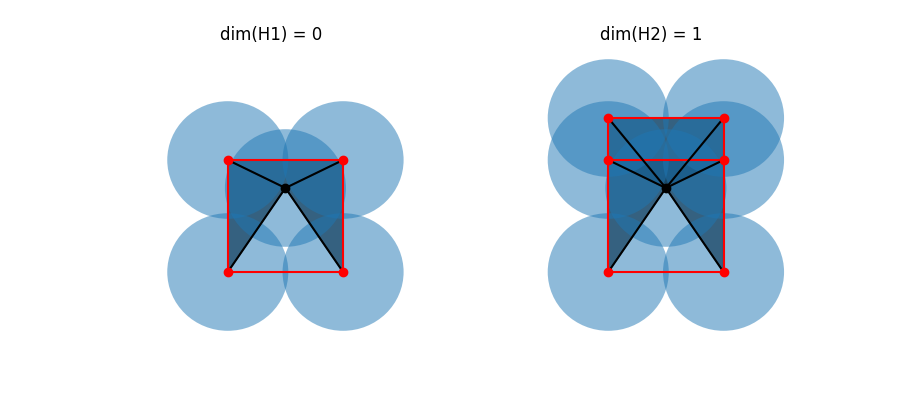
\includegraphics[scale=0.7]{figures/counter.png}
\end{figure}

\paragraph{Fake cycles}
Second, consider a situation in which $P^\delta$ covers $\D$ but there is an additional cycle in $\hom_1(Q^\delta)$ that does not reflect a feature of $\hom_1(\B)$.
In this case there is some point $x\in\D$ surrounded by this cycle that is covered by a point in $P\setminus Q$ but not $Q$.
The result is a non-zero element in $\hom_2(P^\delta, Q^\delta)$ that reflects the void containing this point and not the void corresponding to an element of $\hom_2(\D,\B)$, leading us to a false positive.
Fortunately, this situation is resolved by once again looking at the inclusion $(P^\delta, Q^\delta)\hookrightarrow (P^\gamma, Q^\gamma)$ as any such ``spurious'' cycles are killed for sufficiently large $\gamma > 0$.
This inclusion is contained in the inclusion of Rips complexes $\rips_\delta(P, Q)\hookrightarrow\rips_{2\gamma}(P, Q)$ as follows
\[ \rips_\delta(P, Q) \hookrightarrow \cech_\delta(P,Q)\hookrightarrow\cech_\gamma(P,Q)\hookrightarrow\rips_{2\gamma}(P, Q). \]

\subsection{What do we have? How can we use it?}

The components required to verify a network covers a bounded domain can be summarized by the following
\begin{enumerate}
    \item[a.] the boundary is adequately covered,
    \item[b.] the interior of the domain is covered.
\end{enumerate}
Condition (b) relies on condition (a) in order to provide a topological condition for \emph{coverage} that is necessary but not sufficient.
That is, it can verify coverage alone without false positives but may encounter false negatives.
In fact, the TCC tests a more specific problem: whether we have a reliable representation of the boundary \emph{and} a reliable representation of the interior.

As we have seen, this can be achieved by a collection of sensors that can detect the presence of neighboring sensors at two scales \emph{and} the presence of the boundary.
In reality, it is natural to assume we would like to confirm coverage of a domain in order to measure some quantity.
We therefore consider a situation in which sensors can measure some scalar value, representing a sample of a function defined on the domain.
By defining the boundary in terms of this function we no longer need to require that sensors can detect the presence of the boundary.
Specifically, we can replace the boundary of the domain with a sub-level set that resembles a boundary with specific topological properties.
The points close to the boundary can then be taken as the points measuring function values within a certain range.

In the following section we formalize the notion of a sub-level set resembling a boundary and state the conditions required to confirm coverage.
We then re-state the TCC as a condition that is both necessary \emph{and} sufficient for a more specific problem.% and show how it can be used to approximate the relative persistent homology of the function.
% Finally, we consider classes of functions which satisfy the assumptions made.
% Namely, we consider functions with multiple sub-level sets which may serve as a boundary for this procedure and show how they can be integrated to give a more robust signature for the function.

  %
  % \section{The Topological Coverage Criterion}
  % % !TeX root = main.tex

\subsection{Assumptions}\label{ssec:assumptions}

We first generalize the notion of the topological boundary in the preceding example to the notion of a set which surrounds our domain.

Let $X\subset \R^d$ and $A\subset X$.
We say that $A$ \textbf{separates} $X$ if there exists a pair $(\I, \O)$ such that
\begin{itemize}
    \item $\I, A, \O$ are disjoint,
    \item $\I \cup \O = X\setminus A$,
    \item there is no path from $\I$ to $\O$ that does not cross $A$.
\end{itemize}

\begin{lemma}
    If $A$ separates $X$ with the pair $(\I, \O)$ then for all $k\geq 0$
    \[ \hom_k(\I)\cong\hom_k(\overline{A}, \O). \]
\end{lemma}
% \begin{proof}
%     If $A$ separates $X$ with the pair $(\I, \O)$ then $\I$ and $\O$ are not path connected and $\overline{A} = \I\cup\O$.
%
%     For all $k > 0$ suppose $[x]\in \hom_k(\overline{A}, \O)$ is non-trivial.
%     Because $\I$ and $\O$ are not path connected $\partial x \in C_{k-1}(\O)$ implies that $x\in C_k(\O)$ and therefore that $[x]$ is trivial in $\hom_k(\overline{A}, \O)$.
%     So $[x]$ is not a relative cycle and therefore $[x]\in \hom_k(\overline{A})$, $[x]\notin\hom_k(\O)$.
%     Because $\I$ and $\O$ are not path connected $[x]\notin\hom_k(\O)$ implies $[x]\in \hom_k(\overline{A}\setminus\O) = \hom_k(\I)$.
%
%     On the other hand, if $[x]\in \hom_k(\I)$ then $[x]\in \hom_k(\overline{A}, \I)$ as $\I\subset\overline{A}$ and, because $\I$ and $\O$ are not path connected, $[x]$ is trivial in $\hom_k(\overline{A}, \O)$ if and only if $[x]$ is trivial in $\hom_k(\I)$.
% \end{proof}

\begin{lemma}\label{lem:surrounds}
    If $A$ separates $X$ with the pair $(\I, \O)$ then for all $k\geq 0$, $\e > 0$
    \[\hom_k(\I\setminus A^\e)\cong \hom_k(\overline{A^\e}, \overline{\I^\e}).\]
\end{lemma}

We say that a subset $A$ \textbf{surrounds} $X$ if $A$ separates $\R^d$ with the pair $(X\setminus A, \overline{X})$.

\begin{lemma}\label{lem:surrounds}
    If $A$ surrounds $X$ then for all $\e > 0$
    \[\hom_0((\D\setminus\B^\e,\emptyset)\hookrightarrow (\overline{\B^\e}, \overline{\D^\e}))\]
    is an isomorphism.
\end{lemma}

\subsection{The Topological Coverage Criterion}

Let $\omega,\delta,\gamma \in \R$ such that $U_{\omega-2c\delta}$ is closed and surrounds $\D$, and $\gamma \geq 3\delta$ is such that we have the following sequence of inclusions
\[\D_{\omega - 2c\delta}\subset \D_{\omega - 2c\delta}^{2\delta} \subset \D_{\omega - 2c\delta}^{\delta + \gamma} \subset \D_{\omega + 2c\delta}.\]
In the following let $\B = \D_{\omega - 2c\delta}$.

Let $P$ be a finite subset of $\D$ and $Q = P\cap U_{\omega - c\delta}$.
We have the following commutative diagrams of inclusions between the pairs $(P,Q)$ and $(\D, \B)$ and their complements with increasing scale.

\[ \begin{tikzcd}
(P^\delta, Q^\delta) \arrow[hookrightarrow]{r}\arrow[hookrightarrow]{d}& (P^\gamma, Q^\gamma) \arrow[hookrightarrow]{d} \\%
(\D^{2\delta}, \B^{2\delta}) \arrow[hookrightarrow]{r} & (\D^{\delta+\gamma}, \B^{\delta+\gamma}),
\end{tikzcd}
\begin{tikzcd}
(\overline{\B^{\delta+\gamma}}, \overline{\D^{\delta+\gamma}})\arrow[hookrightarrow]{r}{j}\arrow[hookrightarrow]{d}& (\overline{\B^{2\delta}}, \overline{\D^{2\delta}}) \arrow[hookrightarrow]{d} \\%
(\overline{Q^\gamma}, \overline{P^\gamma}) \arrow[hookrightarrow]{r}{i} & (\overline{Q^\delta}, \overline{P^\delta}).
\end{tikzcd}\]

The following diagram is formed by applying the homology functor.
\[ \begin{tikzcd}\label{dgm:1}
\hom_0(\overline{\B^{\delta+\gamma}}, \overline{\D^{\delta+\gamma}})\arrow{r}{j_*}\arrow{d}& \hom_0(\overline{\B^{2\delta}}, \overline{\D^{2\delta}}) \arrow{d} \\%
\hom_0(\overline{Q^\gamma}, \overline{P^\gamma}) \arrow{r}{i_*} & \hom_0(\overline{Q^\delta}, \overline{P^\delta}).
\end{tikzcd}\]
Let $p_* : \im~j_*\to\im~i_*$.

\begin{theorem}[Geometric TCC]\label{thm:tcc}
    If $\im~\hom_k(\D_{\omega-2c\delta}\hookrightarrow \D_{\omega+{2c\delta}})\cong \hom_k(\D_{\omega - 2c\delta}^{2\delta})$ and $p_*$ is injective then $\D\setminus\D_{\omega-2c\delta}^{2\delta}\subseteq P^\delta$ and $Q^\delta$ separates $\D$.
\end{theorem}

\begin{corollary}
    If $\im~\hom_k(\D_{\omega-2c\delta}\hookrightarrow \D_{\omega+{2c\delta}})\cong \hom_k(\D_{\omega - 2c\delta}^{2\delta})$ and $p_*$ is injective then for all $k\geq 0$
    \[ \im~i_* \cong \hom_k(\D^{2\delta}, \B^{2\delta}).\]
\end{corollary}

% \begin{lemma}\label{lem:separate}
%     If $j_*$ is surjective and $p_*$ is injective then $Q^\delta$ separates $\D$.
% \end{lemma}
% \begin{proof}
%     Suppose, for the sake of contradiction, that $Q^\delta$ does not separate $\D$.
%     Then for all $(\I, \O)$ such that $\I \cup \O = \D\setminus Q^\delta$ there must exist some path from $\I$ to $\O$ that does not cross $Q^\delta$.
%     Formally, there exists a path $\pi : [0,1]\to\overline{Q^\delta}$ with $\pi(0)\in \I$ and $\pi(1)\in\O$.
%     Noting that $\overline{\B^{2\delta}}\subseteq \overline{Q^\delta}$ and, because $\overline{\B^{2\delta}} = \overline{\D^{2\delta}}\cup (\D\setminus\B^{2\delta})$ surrounds $\D^{2\delta}$ we can choose $(\I, \O)$ such that $\D\setminus \B^{2\delta}\subset \I$ and $\overline{\D^{2\delta}}\subset \O$.
%
%     Choose $x\in\D\setminus \B^{2\delta}$ and $y\in \overline{\D^{2\delta}}$ such that there exist paths $\pi_x : [0,1]\to \I$ with $\pi_x(0) = x$, $\pi_x(1) = \pi(0)$ and $\pi_y : [0,1]\to \O$ with $\pi_y(0) = y$, $\pi_y(1) = \pi(1)$.
%     $\pi_x, \pi_y$ and $\pi$ all generate chains in $C_1(\overline{Q^\delta}, \overline{P^\delta})$ and $\pi_x + \pi + \pi_y = \pi^*\in C_1(\overline{Q^\delta}, \overline{P^\delta})$ with $\partial\pi^* = x + y$.
%     Moreover, $y$ generates a chain in $C_0(\overline{P^\delta})$ as $\overline{\D^{2\delta}}\subseteq\overline{P^\delta}$.
%     So $x = \partial\pi^* + y$ is a relative boundary in $C_0(\overline{Q^\delta}, \overline{P^\delta})$ thus $[x] = 0 = [y]$ in $\hom_0(\overline{Q^\delta}, \overline{P^\delta})$ and therefore $[x] = [y]$ in $\im~i_*$.
%     However, because $\B^{2\delta}$ separates $\D$ with the pair $(\overline{\D^{2\delta}}, \D\setminus\B^{2\delta})$ we know that $[x]\neq [y]$ in $\hom_0(\overline{\B^{2\delta}}, \overline{\D^{2\delta}})\cong \im~j_*$, contradicting our assumption that $p_*$ is injective.
% \end{proof}
%
% In the following we will assume that $j_*$ is surjective and $p_*$ is injective.
% By Lemma~\ref{lem:separate} $Q^\delta$ separates $\D$ with a pair $(\I, \O)$.
% Let $\hat{Q}^\delta = Q^\delta \cup \O$, $\hat{P}^\delta = P^\delta \cup \O$ and $\hat{Q}^\gamma = Q^\gamma \cup \O$.
%
% \begin{lemma}
%     $\hom_*(\hat{P}^\delta, \hat{Q}^\delta)\cong \hom_*(P^\delta, Q^\delta)$ and $\hom_*(P^\delta\cup\hat{Q}^\gamma, \hat{Q}^\gamma)\cong \hom_*(P^\delta\cup Q^\gamma, Q^\gamma)$.
% \end{lemma}
% \begin{proof}
%     By the definition of $\hat{Q}^\delta$, $\hat{Q}^\gamma$ and $\O$ we have that $\hat{Q}^\delta\setminus\O = Q^\delta$ and $\hat{Q}^\gamma\setminus\O = Q^\gamma$ and $\cl~\O \subset \intr~\hat{Q}^\delta, \intr~\hat{Q}^\gamma$.
%     The desired results follow by Excision.
% \end{proof}
%
% \begin{lemma}
%     If $p_*$ is injective then $\B^{2\delta}\subseteq \hat{Q}^\gamma$.
% \end{lemma}
% \begin{proof}
%     Suppose $p_*$ is injective and there exists some $x\in \B^{2\delta}$ such that $x\notin \hat{Q}^\gamma$.
%     So there exists some $y\in U_{\omega - 2c\delta}$ such that $\dist(x, y) < 2\delta$.
%     Because $Q^\delta$ separates $\D = \O \cup Q^\delta \cup \I$ both $x$ and $y$ are either in $Q^\delta, \O$ or $\I$.
%     Moreover, $\overline{\I} = Q^\delta \cup \O = \hat{Q}^\delta$ so $\B^{2\delta}\cap\I = \B^{2\delta}\setminus \hat{Q}^\delta$ and $\B\cap\I = \B\setminus \overline{\I} = \B\setminus \hat{Q}^\delta = \emptyset$ as $\B\subset \hat{Q}^\delta$.
%     So $y\notin \I$ and, because $Q^\delta \subset Q^\gamma$ and $\O\subset \hat{Q}^\delta\subset\hat{Q}^\gamma$, we can assume w.l.o.g. that $x\in \B^{2\delta}\cap\I$.
%
%     If $y\in Q^\delta$ then there exists some $q\in Q$ such that $\dist(q, y) < \delta$ so
%     \[ \dist(q, x)\leq \dist(q, y) + \dist(x, y) < 3\delta\leq\gamma \]
%     which implies $x \in Q^\gamma$.
%
%     So we may assume that $y\in U_{\omega - 2c\delta}\cap\O$.
%     Because $Q^\delta$ separates $\D$ with $(\I, \O)$ there is no path from $x\in \I$ to $y\in\O$ that does not cross $Q^\delta$, so there must be some point $z\in Q^\delta$ in the shortest path from $x$ to $y$.
%     That is, there exists some $q\in Q$ such that $\dist(q, z) < \delta$ and $\dist(z, x) < \dist(x, y) < 2\delta$ so
%     \[ \dist(q, x)\leq \dist(q, z) + \dist(z, x) < \delta + 2\delta \leq \gamma. \]
%     So $y\in\O$ implies $x\in\hat{Q}^\gamma$.
%
% \end{proof}

  % % !TeX root = main.tex

\subsection{Proof of the TCC}

\begin{lemma}\label{lem:jsurj}
    Given assumptions 1-3 the map $j_*$ is surjective.
\end{lemma}
\begin{proof}
    \textbf{TODO this true?
    What other conditions do we need for it to be true?
    Do we have to assume this as well?}
\end{proof}

\begin{lemma}\label{lem:psurj}
    Given assumptions 1-3, the map $p_*$ is surjective.
\end{lemma}
\begin{proof}
    \textbf{TODO Do we even need this?
    If $\im~i_*$ is finite-dimensional and $\rk~i_* \geq \rk~j_*$ is $p_*$ injective?
    We can also just state the theorem as ``if $p_*$ is injective.''}
\end{proof}
% \begin{proof}
%     By Lemma~\ref{lem:jsurj} $j_*$ is surjective.
%     Choose a basis for $\im~i_*$ such that each basis element is represented by a point in $P^\delta\setminus Q^\gamma$.
%     Let $x\in P^\delta\setminus Q^\gamma$ be such that $[x]$ is non-trivial in $\im~i_*$.
%     Suppose $x\in\B^{2\delta}$ and let $y\in\B$ such that $\dist(x, y)< 2\delta$.
%
%     First, suppose $y\in P^\delta$.
%     So there exists some $p\in P$ such that $\dist(p, y) < \delta$.
%     But $y\in \B = \D_{\omega-2c\delta}$ so $f(y)\leq \omega-2c\delta$.
%     Therefore, because $f$ is $c$-Lipschitz
%     \[ f(p) \leq c\dist(p, y) + f(y) < \omega - 2c\delta + c\delta = \omega - c\delta\]
%     so $p\in Q$, thus $y\in Q^\delta$.
%     So $y\in P^\delta$ implies $y\in Q^\delta$ and therefore, by contrapositive, $y\in\overline{Q^\delta}$ implies $y\in\overline{P^\delta}$.
%
%     Now, because $x\in\overline{Q^\gamma}$ by hypothesis $\dist(x, q) \geq \gamma$ for all $q\in Q$.
%     For any $z$ in the shortest path between $x$ and $y$ we have $\dist(x, z)\leq \dist(x, y) < 2\delta$, so the following inequality holds for all $q\in Q$
%     \begin{align*}
%         \dist(x, q) &\geq \dist(x, q) - \dist(x, z)\\
%         &> \gamma - 2\delta\\
%         &\geq \delta.
%     \end{align*}
%     So $z\in \overline{Q^\delta}$ for all $z$ in the shortest path from $x$ to $y$.
%     In particular, $x,y\in\overline{Q^\delta}$ therefore $y\in\overline{P^\delta}$.
%
%     Because $x,y\in\overline{Q^\delta}$ we have corresponding chain $x,y\in C_0(\overline{Q^\delta})$ and $y\in\overline{P^\delta}$ generates a chain $y\in C_0(P^\delta)$.
%     As we have shown that $x\in \B^{2\delta}$ implies that the shortest path from $x$ to $y$ is contained in $\overline{Q^\delta}$ there exists a path $h: [0,1]\to \overline{Q^\delta}$ with $h(0) = x$ and $h(1) = y$ that generates a chain $h\in C_1(\overline{Q^\delta})$.
%     So for $h\in C_1(\overline{Q^\delta}, \overline{P^\delta})$ with $\partial h = x + y$ we have that $x = \partial h + y$.
%     Thus $[x]$ is a relative boundary and is therefore trivial in $\hom_0(\overline{P^\delta}, \overline{Q^\delta})$, a contradiction, as we have assumed $[x]$ is non-trivial in $\im~i_*$.
%     So we may conclude that $x\notin \B^{2\delta}$.
%
%     So $x\in\overline{\B^{2\delta}}$ and $x\in \D\setminus\B^{2\delta}$.
%     So $[x]$ is non-trivial in $\hom_0(\overline{\B^{2\delta}},\overline{\D^{2\delta}})$ and, because $j_*$ is surjective, $\im~j_* = \hom_0(\overline{\B^{2\delta}},\overline{\D^{2\delta}})$.
%     So $p_*$ is surjective as $p_*[x] = [x]\in\im~p_*$ for all non-trivial $[x]\in\im~i_*$.
% \end{proof}

\begin{lemma}\label{lem:coverage}
    Given assumptions 1-3, if $p_*$ is injective then $\D\setminus\B^{2\delta}\subseteq P^\delta$.
\end{lemma}
\begin{proof}
    Suppose, for the sake of contradiction, that $p_*$ is injective and there exists a point $x\in (\D\setminus\B^{2\delta})\setminus P^\delta$.
    So $[x]$ is non-trivial in $\hom_0(\overline{\B^{2\delta}},\overline{\D^{2\delta}}) = \im~j_*$ as $x$ is in some connected component of $\D\setminus\B^{2\delta}$ and $j_*$ is surjective.
    So we have the following sequence of maps induced by inclusions
    \[ \hom_0(\overline{\B^{2\delta}},\overline{\D^{2\delta}})\xrightarrow{f_*} \hom_0(\overline{\B^{2\delta}},\overline{\D^{2\delta}}\cup\{x\})\xrightarrow{g_*} \hom_0(\overline{Q^\delta},\overline{P^\delta}).\]
    As $f_*[x]$ is trivial in $\hom_0(\overline{\B^{2\delta}},\overline{\D^{2\delta}}\cup\{x\})$ we have that $p_*[x] = (g_*\circ f_*)[x]$ is trivial, contradicting our hypothesis that $p_*$ is injective.
\end{proof}

\begin{lemma}\label{lem:separate}
    Given assumptions 1-3, if the map $p_*$ is injective then $Q^\delta$ separates $\D$.
\end{lemma}
\begin{proof}
    Suppose, for the sake of contradiction, that $Q^\delta$ does not separate $\D$.
    Then for all $(\I, \O)$ such that $\I \cup \O = \D\setminus Q^\delta$ there must exist some path from $\I$ to $\O$ that does not cross $Q^\delta$.
    Formally, there exists a path $\pi : [0,1]\to\overline{Q^\delta}$ with $\pi(0)\in \I$ and $\pi(1)\in\O$.
    Noting that $\overline{\B^{2\delta}}\subseteq \overline{Q^\delta}$ and, because $\overline{\B^{2\delta}} = \overline{\D^{2\delta}}\cup (\D\setminus\B^{2\delta})$ surrounds $\D^{2\delta}$ we can choose $(\I, \O)$ such that $\D\setminus \B^{2\delta}\subset \I$ and $\overline{\D^{2\delta}}\subset \O$.

    Choose $x\in\D\setminus \B^{2\delta}$ and $y\in \overline{\D^{2\delta}}$ such that there exist paths $\pi_x : [0,1]\to \I$ with $\pi_x(0) = x$, $\pi_x(1) = \pi(0)$ and $\pi_y : [0,1]\to \O$ with $\pi_y(0) = y$, $\pi_y(1) = \pi(1)$.
    $\pi_x, \pi_y$ and $\pi$ all generate chains in $C_1(\overline{Q^\delta}, \overline{P^\delta})$ and $\pi_x + \pi + \pi_y = \pi^*\in C_1(\overline{Q^\delta}, \overline{P^\delta})$ with $\partial\pi^* = x + y$.
    Moreover, $y$ generates a chain in $C_0(\overline{P^\delta})$ as $\overline{\D^{2\delta}}\subseteq\overline{P^\delta}$.
    So $x = \partial\pi^* + y$ is a relative boundary in $C_0(\overline{Q^\delta}, \overline{P^\delta})$ thus $[x] = 0 = [y]$ in $\hom_0(\overline{Q^\delta}, \overline{P^\delta})$ and therefore $[x] = [y]$ in $\im~i_*$.
    However, because $\B^{2\delta}$ separates $\D$ with the pair $(\overline{\D^{2\delta}}, \D\setminus\B^{2\delta})$ we know that $[x]\neq [y]$ in $\hom_0(\overline{\B^{2\delta}}, \overline{\D^{2\delta}})\cong \im~j_*$, contradicting our assumption that $p_*$ is injective.
\end{proof}

\begin{theorem}[Geometric TCC]\label{thm:tcc}
    Let $\D\subset\R^d$ and $f:\D\to\R$ be a $c$-Lipschitz function satisfying assumptions 1-3 for $\omega\in\R$, $\delta > 0$, and $\gamma > 3\delta$.
    Let $P\subset\D$ be a collection of sensors and let $Q = P\cap \D_{\omega - c\delta}$, $\B = \D_{\omega - 2c\delta}$.
    Let $p_* : \im~j_*\to\im~i_*$ for $j_*$, $i_*$ as defined in Diagram~\ref{dgm:1}.

    If $\rk~i_*\geq \rk~j_*$ then $\D\setminus\B^{2\delta}\subseteq P^\delta$ and $Q^\delta$ separates $\D$.
\end{theorem}
\begin{proof}
    % Lemma~\ref{lem:psurj} states that $p_*$ is surjective so $p_*$ is surjective, so $\rk~i_*\leq \rk~j_*$.
    % Because $\rk~i_*\geq \rk~j_*$, $$\rk~i_* = \rk~j_*$.
    Because $P$ is a finite point set we know that $\im~i_*$ is finite-dimensional.
    Because $\rk~i_*\geq \rk~j_*$ $j_*$ is finite dimensional as well so $p_*$ is injective.
    Therefore $\D\setminus\B^{2\delta}\subseteq P^\delta$ by Lemma~\ref{lem:coverage} and $Q^\delta$ separates $\D$ by Lemma~\ref{lem:separate}.
\end{proof}

  % % !TeX root = main.tex

\subsection{Proof of the Interleaving}

In the following we will assume that $j_*$ is surjective and $p_*$ is injective.
By Lemma~\ref{lem:separate} $Q^\delta$ separates $\D$ with a pair $(\I, \O)$.
Let $\hat{Q}^\delta = Q^\delta \cup \O$, $\hat{P}^\delta = P^\delta \cup \O$ and $\hat{Q}^\gamma = Q^\gamma \cup \O$.

\begin{lemma}
    $\hom_*(\hat{P}^\delta, \hat{Q}^\delta)\cong \hom_*(P^\delta, Q^\delta)$ and $\hom_*(P^\delta\cup\hat{Q}^\gamma, \hat{Q}^\gamma)\cong \hom_*(P^\delta\cup Q^\gamma, Q^\gamma)$.
\end{lemma}
\begin{proof}
    By the definition of $\hat{Q}^\delta$, $\hat{Q}^\gamma$ and $\O$ we have that $\hat{Q}^\delta\setminus\O = Q^\delta$ and $\hat{Q}^\gamma\setminus\O = Q^\gamma$ and $\cl~\O \subset \intr~\hat{Q}^\delta, \intr~\hat{Q}^\gamma$.
    The desired results follow by Excision.
\end{proof}

\begin{lemma}\label{lem:qcontain}
    If $p_*$ is injective then $\B^{2\delta}\subseteq \hat{Q}^\gamma$.
\end{lemma}
\begin{proof}
    Suppose $p_*$ is injective and there exists some $x\in \B^{2\delta}$ such that $x\notin \hat{Q}^\gamma$.
    So there exists some $y\in U_{\omega - 2c\delta}$ such that $\dist(x, y) < 2\delta$.
    Because $Q^\delta$ separates $\D = \O \cup Q^\delta \cup \I$ both $x$ and $y$ are either in $Q^\delta, \O$ or $\I$.
    Moreover, $\overline{\I} = Q^\delta \cup \O = \hat{Q}^\delta$ so $\B^{2\delta}\cap\I = \B^{2\delta}\setminus \hat{Q}^\delta$ and $\B\cap\I = \B\setminus \overline{\I} = \B\setminus \hat{Q}^\delta = \emptyset$ as $\B\subset \hat{Q}^\delta$.
    So $y\notin \I$ and, because $Q^\delta \subset Q^\gamma$ and $\O\subset \hat{Q}^\delta\subset\hat{Q}^\gamma$, we can assume w.l.o.g. that $x\in \B^{2\delta}\cap\I$.

    If $y\in Q^\delta$ then there exists some $q\in Q$ such that $\dist(q, y) < \delta$ so
    \[ \dist(q, x)\leq \dist(q, y) + \dist(x, y) < 3\delta\leq\gamma \]
    which implies $x \in Q^\gamma$.

    So we may assume that $y\in U_{\omega - 2c\delta}\cap\O$.
    Because $Q^\delta$ separates $\D$ with $(\I, \O)$ there is no path from $x\in \I$ to $y\in\O$ that does not cross $Q^\delta$, so there must be some point $z\in Q^\delta$ in the shortest path from $x$ to $y$.
    That is, there exists some $q\in Q$ such that $\dist(q, z) < \delta$ and $\dist(z, x) < \dist(x, y) < 2\delta$ so
    \[ \dist(q, x)\leq \dist(q, z) + \dist(z, x) < \delta + 2\delta \leq \gamma. \]
    So $y\in\O$ implies $x\in\hat{Q}^\gamma$.

\end{proof}

The following lemma is a well-established result that we provide without proof.

\begin{lemma}[Lemma 3.2 from~\cite{chazal08towards}]\label{lem:sandwich}
    Given a sequence $A\to B\to C\to D\to E\to F$ of homomorphisms between finite-dimensional vector spaces, if $\rk(A\to F) = \rk(C\to D)$ then this quantity also equals the rank of $B\to E$.
    Similarly, if $A\to B\to C\to E\to F$ is a sequence of homomorphisms such that $\rk(A\to F) = \dim~C$ then $\rk(B\to E) = \dim~C$.
\end{lemma}

% \begin{lemma}
%     If $p_*$ is injective then $\im~\hom_*(P^\delta\to (P^\delta\cup \hat{Q}^\gamma)\setminus\B)\cong \hom_*(\D\setminus\B^{2\delta})$.
% \end{lemma}
% \begin{proof}
%     \textbf{TODO requires \[ \D\setminus \B^{2\delta} \subseteq P^\delta \subseteq P^\delta \cup U_{\omega - 2c\delta}^{2\delta}\subseteq P^\delta\cup \hat{Q}^\gamma \subseteq \D \] and $\im~\hom_*(\D\setminus \B^{2\delta} \to \D)\cong\hom_*(P^\delta \cup U_{\omega - 2c\delta}^{2\delta}) = \hom_*(\D)$.}
% \end{proof}
% % \begin{proof}
% %     First note that because $p_*$ is injective $\D\setminus\B^{2\delta}\subseteq P^\delta$ and because $\B^{2\delta}\subseteq U_\omega$ we have $\D\setminus U_\omega \subseteq \D\setminus \B^{2\delta} \subseteq P^\delta$.
% %     We have the following sequence of inclusions
% %     \[ \D\setminus U_\omega \subseteq P^\delta \subseteq P^\delta \cup U_{\omega - 2c\delta}^{2\delta}\subseteq P^\delta\cup \hat{Q}^\gamma \subseteq \D \]
% %     which induces the following sequence of homomorphisms
% %     \[ \hom_*(\D\setminus U_\omega)\to\hom_*(P^\delta\setminus\B)\to\hom_*((P^\delta \cup \B^{2\delta})\setminus \B)\to\hom_*((P^\delta\cup\hat{Q}^\gamma)\setminus\B)\to\hom_*(\D\setminus\B).\]
% %     As $\D\setminus\B^{2\delta}\subseteq P^\delta$ implies $P^\delta\cup\B^{2\delta} = \D$ and $\hom_*(\D\setminus U_\omega)\cong \hom_*(\D\setminus \B)$ we have that $\im~\hom_*(\D\setminus U_\omega\to \D\setminus \B)\cong \hom_*(\D\setminus\B)$ and therefore $\im~\hom_*(P^\delta\to(P^\delta\cup\hat{Q}^\gamma)\setminus\B)\cong\hom_*(\D\setminus \B)$ by Lemma~\ref{lem:sandwich}.
% % \end{proof}

\begin{lemma}
    Given assumptions 1-3, if $p_*$ is injective then $\im~\hom_*(\hat{Q}^\delta \to \hat{Q}^{\gamma})\cong \hom_*(\B^{2\delta}).$
\end{lemma}
\begin{proof}
    By assumption 3 $\D_{\omega-c\delta}^\delta\to \D_{\omega-2c\delta}^{2\delta}$ is a deformation retraction so $\hom_*(\D_{\omega-c\delta}^\delta)\to \hom_*(\D_{\omega-2c\delta}^{2\delta})$ is an isomorphism.
    As $Q = P\cap \D_{\omega-c\delta}$ we have that $\hat{Q}^\delta\subset \D_{\omega-c\delta}^\delta$ and $\hat{Q}^\gamma\subset\D_{\omega - c\delta}^\gamma\subset \D_{\omega + 2c\delta}$ by assumption 4.
    If $p_*$ is injective we know that $\D_{\omega - 2c\delta}^{2\delta}\subseteq \hat{Q}^\gamma$ by Lemma~\ref{lem:qcontain} so we have the following sequence of homomorphisms
    \[ \hom_*(\D_{\omega - 2c\delta})\to \hom_*(\hat{Q}^\delta)\to \hom_*(\D_{\omega-c\delta}^\delta)\to \hom_*(\D_{\omega - 2c\delta}^{2\delta})\to\hom_*(\hat{Q}^\gamma)\to\hom_*(\D_{\omega + 2c\delta}).\]
    By assumption 2 $\im~\hom_*(\D_{\omega - 2c\delta}\hookrightarrow U_{\omega+2c\delta})\cong\hom_*(U_{\omega-2c\delta}^{2\delta})$ so \[\hom_*(\hat{Q}^\delta\hookrightarrow\hat{Q}^\gamma)\cong\hom_*(\D_{\omega-c\delta}^\delta\to \D_{\omega-2c\delta}^{2\delta})\cong \hom_*(\B^{2\delta})\] by Lemma~\ref{lem:sandwich}.
\end{proof}

\begin{lemma}
    Given assumption 2, if $p_*$ is injective then $\im~\hom_*(P^\delta\setminus \B^{2\delta} \to P^\delta\setminus \B)\cong \hom_*(\D\setminus\B^{2\delta}).$
\end{lemma}
\begin{proof}
    If $p_*$ is injective we have the following sequence of homomorphisms induced by inclusion
    \[\hom_*(\D\setminus\D_{\omega+2c\delta})\to\hom_*(P^\delta\setminus \B^{2\delta})\to\hom_*(\D\setminus\B^{2\delta})\to\hom_*(P^\delta\setminus \B)\to\hom_*(\D\setminus\B).\]
    By assumption 2 $\hom_*(\D\setminus\D_{\omega+2c\delta}\hookrightarrow \D\setminus\B)\cong\hom_*(\D\setminus\B^{2\delta})$ so $\im~\hom_*(P^\delta\setminus \B^{2\delta} \to P^\delta\setminus\B)\cong \hom_*(\D\setminus\B^{2\delta})$ by Lemma~\ref{lem:sandwich}.
\end{proof}


\section{Future Work}

Conformation of the TCC implies that we cover the interior of the domain $\D\setminus\B^{2\delta}$ and that $Q^\delta$ separates $\D$ which.
As we have shown, this implies that the inclusion our sampled boundary at scales $\delta,\gamma$ captures the homology of the thickened boundary $\B^{2\delta}$ and the inclusion of our sampled interior captures the homology of the interior $\D\setminus\B^{2\delta}$.
However, this alone does not imply that the inclusion of pairs $(P^\delta, Q^\delta)\to (P^\gamma, Q^\gamma)$ captures the \emph{relative} homology of the pair $(\D,\B^{2\delta})$ as it does not account for homological features that may appear only in relative homology.
Specifically, any principal homology classes in $\hom_*(\D)$ that become relative homology classes in $\hom_*(\D\setminus\B^{2\delta}, \D_{\omega +2c\delta}\setminus \B^{2\delta})$ may not occur \emph{at all} in $\hom_*(P^\delta, Q^\delta)$.
Identifying additional assumptions or side-effects of the TCC is the subject of future work, and would allow us to prove Lemma~\ref{lem:broken} and Theorem~\ref{thm:scalar}.

% , as we have shown, implies that $\B^{2\delta}\subset Q^\delta$ and the inclusions $\hom_*(\hat{Q}^\delta\hookrightarrow\hat{Q}^\gamma)$ and $\im~\hom_*(P^\delta\setminus \B^{2\delta} \to P^\delta\setminus \B)$ are isomorphic to $\hom_*(\B^{2\delta})$ and $\hom_*(\D\setminus\B^{2\delta})$ respectively.
% That is, the inclusion of our sampled boundary serv

% \begin{lemma}
%     If $\im~\hom_*(\hat{Q}^\delta\to\hat{Q}^\gamma)\cong\hom_*(\B^{2\delta})$ and $\im~\hom_*(P^\delta\setminus\B\to (P^\delta\cup \hat{Q}^\gamma)\setminus\B)\cong \hom_*(\D\setminus\B^{2\delta})$ then
%     \[\im~\hom_*((P^\delta, Q^\delta)\to (P^\delta\cup Q^\gamma, Q^\gamma))\cong \hom_*(\D, \B). \]
% \end{lemma}

\begin{lemma}~\label{lem:broken}
    If $\im~\hom_*(\hat{Q}^\delta\to\hat{Q}^\gamma)\cong\hom_*(\B^{2\delta})$ and $\im~\hom_*(P^\delta\setminus Q^\gamma \to P^\delta\setminus Q^\delta)\cong \hom_*(\D\setminus\B^{2\delta})$ then
    \[\im~\hom_*((P^\delta, Q^\delta)\to (P^\delta\cup Q^\gamma, Q^\gamma))\cong \hom_*(\D^{2\delta}, \B^{2\delta}). \]
\end{lemma}

\begin{theorem}\label{thm:scalar}
    If $\im~\hom_*((P^\delta, Q^\delta)\to (P^\delta\cup Q^\gamma, Q^\gamma))\cong \hom_*(\D^{2\delta}, \B^{2\delta})$ then \[\{(P_\alpha^\delta, Q^\delta)\to (P_\alpha^\delta\cup Q^\gamma, Q^\gamma)\}_{\alpha > \omega+2c\delta}\] is $c\delta$-interleaved with $\{(\D_\alpha, \B^{2\delta})\}_{\alpha > \omega +2c\delta}$.
\end{theorem}

  % % !TeX root = ../../main.tex

\subsection{Some Helpful Lemmas}

% \begin{lemma}[Splitting Lemma (Hatcher p. 147)]\label{lem:splitting}
%   For a short exact sequence \[0\to A\xrightarrow{i} B\xrightarrow{j} C\to 0\] of abelian groups the following statements are equivalent
%   \begin{enumerate}
%     \item There is a homomorphism $p: B\to A$ such that $p\circ i = \mathbf{Id}_A$.
%     \item There is a homomorphism $s: C\to B$ such that $j\circ s = \mathbf{Id}_C$.
%     \item There is an isomorphism $B\cong A\oplus C$ making the commutative diagram below, where the maps in the lower row are the obvious ones $a\mapsto (a, 0)$ and $(a,c)\mapsto c$.
%
%     \[\begin{tikzcd}[column sep=small, row sep=small]
%               &                       & B\ar[dd, "\cong"]\ar[dr,"j"]  &         & \\
%       0\ar[r] & A\ar[ur, "i"]\ar[dr]  &                               & C\ar[r] & 0\\
%               &                       & A\oplus C\ar[ur]              &         &
%     \end{tikzcd}\]
%   \end{enumerate}
% \end{lemma}

\begin{lemma}[\textbf{The Five-Lemma} (Hatcher p. 129)]\label{lem:five}
  In a commutative diagram of abelian groups as below, if the two rows are exact and $\alpha,\beta,\delta$, and $\e$ are isomorphisms then $\gamma$ is an isomorphism.
  \[\begin{tikzcd}
      A\ar[r, "i"]\ar[d, "\alpha"]
    & B\ar[r, "j"]\ar[d, "\beta"]
    & C\ar[r, "k"]\ar[d, "\gamma"]
    & D\ar[r, "\ell"]\ar[d, "\delta"]
    & E\ar[d, "\e"]\\
    %
      A'\ar[r, "i'"]
    & B'\ar[r, "j'"]
    & C'\ar[r, "k'"]
    & D'\ar[r, "\ell'"]
    & E'\\
  \end{tikzcd}\]

  \begin{itemize}
    \item If $\beta$ and $\delta$ are surjective and $\e$ is injective then $\gamma$ is surjective.
    \item If $\beta$ and $\delta$ are injective and $\alpha$ is surjective then $\gamma$ is injective.
  \end{itemize}
\end{lemma}

\begin{theorem}[\textbf{Universal Coefficient Theorem} (Munkres p. 323, Corollary 53.2)]\label{thm:univ_coef}
  Let $(A,B)$ be a topological pair.
  Then for all $k$ and any abelian group $G$ there is a natural exact sequence
  \[ 0\to\mathrm{Ext}(\hom_{k-1}(A, B), G)\to \hom^k(A, B; G)\xrightarrow{\nu} \Hom(\hom_k(A, B), G)\to 0.\]
  This sequence splits, but not naturally.
\end{theorem}

\subsection{A Helpful Diagram}

% \begin{landscape}
% \begin{scriptsize}
% \begin{centering}
% \[\begin{tikzcd}[row sep=large, column sep=scriptsize]
%   |[alias=U]| \D{\omega-c(\delta+\zeta)}{\alpha-3c\delta}
%                                   \arrow[to=V, "\gamma_{\alpha-3c\delta}{[3c\delta]}"]
%                                   \arrow[to=Sa, "f_{\omega-c(\delta+\zeta}{[\alpha-3c\delta]}"]
%   &&&& |[alias=V]| \D{\omega}{\alpha}
%                                   \arrow[to=W, "\pi_\alpha{[3c\zeta]}"]
%                                   \arrow[to=Ta, "f_\omega{[\alpha]}"]
%   &&&& |[alias=W]|
%   \D{\omega+c(\delta+2\zeta)}{\alpha+3c\zeta}\\
%   %
%   & |[alias=Sa]|
%   \P{\omega-c\zeta}{\delta}{\alpha-2c\delta}
%                                   \arrow[to=Sb, "s_{\alpha-2c\delta}"]
%                                   \arrow[to=CSa, "(\E\N_{w-c\zeta}^\delta{[\alpha-2c\delta]})^{-1}"]
%   && |[alias=Sb]| \P{\omega-c\zeta}{2\delta}{\alpha-2c\delta}
%                                   \arrow[to=Ta, "\vartheta_{\alpha-2c\delta}{[2c\delta+\zeta]}"]
%                                   \arrow[to=V, "m_{\omega-c\zeta}^{2\delta}{[\alpha-2c\delta]}"]
%   && |[alias=Ta]| \P{\omega+c\delta}{\zeta}{\alpha+c\zeta}
%                                   \arrow[to=Tb, "t_{\alpha+c\zeta}"]
%                                   \arrow[to=CTa, "(\E\N_{w+c\delta}^\zeta{[\alpha+c\zeta]})^{-1}"]
%   && |[alias=Tb]| \P{\omega+c\delta}{2\zeta}{\alpha+c\zeta}
%                                   \arrow[to=W, "m_{\omega+c\delta}^{2\zeta}{[\alpha+c\zeta]}"]
%   &\\
%   %
%   & |[alias=CSa]|
%   \CP{\omega-c\zeta}{\delta}{\alpha-2c\delta}
%                                   \arrow[to=CSb, "\check{s}_{\alpha-2c\delta}"]
%                                   \arrow[to=RS, "\I_{\omega-c\zeta}^\delta{[\alpha-2c\delta]}"']
%   && |[alias=CSb]| \CP{\omega-c\zeta}{2\delta}{\alpha-2c\delta}
%                                   \arrow[to=Sb, "\E\N_{w-c\zeta}^{2\delta}{[\alpha-2c\delta]}"]
%                                   \arrow[to=CTa, "\check{\vartheta}_{\alpha-2c\delta}{[2c\delta+\zeta]}"]
%   && |[alias=CTa]| \CP{\omega+c\delta}{\zeta}{\alpha+c\zeta}
%                                   \arrow[to=CTb, "\check{t}_{\alpha+c\zeta}"]
%                                   \arrow[to=RT, "\I_{\omega+c\delta}^\zeta{[\alpha+c\zeta]}"']
%   && |[alias=CTb]| \CP{\omega+c\delta}{2\zeta}{\alpha+c\zeta}
%                                   \arrow[to=Tb, "\E\N_{w+c\delta}^{2\zeta}{[\alpha+2c\zeta]}"]
%   &\\
%   %
%   && |[alias=RS]| \CP{\omega-c\zeta}{2\delta}{\alpha-2c\delta}
%                                   \arrow[to=CSb, "\J_{\omega-c\zeta}^{2\delta}{[\alpha-2c\delta]}"]
%                                   \arrow[to=RT, "\rips\lambda_{\alpha-c\zeta}{[c(2\delta+\zeta)]}"]
%   &&&& |[alias=RT]| \RP{\omega+c\delta}{2\zeta}{\alpha+c\zeta}
%                                   \arrow[to=CTb, "\J_{\omega+c\delta}^{2\zeta}{[\alpha+c\zeta]}"]
%   &&\\
% \end{tikzcd}\]
% \end{centering}
% \end{scriptsize}
% \end{landscape}

\begin{scriptsize}
\begin{centering}
\[\begin{tikzcd}[row sep=large, column sep=scriptsize]
  |[alias=U]| \DD{\omega-c(\delta+\zeta)}
                                  \arrow[to=V, two heads, blue, "\Gamma{[3c\delta]}"]
                                  \arrow[to=Sa,blue, "F"]
  &&&& |[alias=V]| \DD{\omega}
                                  \arrow[to=W, hook,red, "\Pi{[3c\zeta]}"]
                                  \arrow[to=Ta,red, "G"]
  &&&& |[alias=W]|
  \DD{\omega+c(\delta+2\zeta)}\\
  %
  & |[alias=Sa]|
  \E\PP{\omega-c\zeta}{\delta}
                                  \arrow[to=Sb, blue, "\mathcal{S}"]
                                  \arrow[to=CSa, "(\E\N_{w-c\zeta}^\delta)^{-1}"]
  && |[alias=Sb]| \E\PP{\omega-c\zeta}{2\delta}
                                  \arrow[to=Ta, "\Theta{[2c\delta+\zeta]}"]
                                  \arrow[to=V, blue, "M"]
  && |[alias=Ta]| \E\PP{\omega+c\delta}{\zeta}
                                  \arrow[to=Tb, red, "\mathcal{T}"]
                                  \arrow[to=CTa, "(\E\N_{w+c\delta}^\zeta)^{-1}"]
  && |[alias=Tb]| \E\PP{\omega+c\delta}{2\zeta}
                                  \arrow[to=W, red, "N"]
  &\\
  %
  & |[alias=CSa]|
  \CPP{\omega-c\zeta}{\delta}
                                  \arrow[to=CSb, green, "\cech\mathcal{S}"]
                                  \arrow[to=RS, green, "\I_{\omega-c\zeta}^\delta"']
  && |[alias=CSb]| \CPP{\omega-c\zeta}{2\delta}
                                  \arrow[to=Sb, "\E\N_{w-c\zeta}^{2\delta}"]
                                  \arrow[to=CTa, "\cech\Theta{[2c\delta+c\zeta]}"]
  && |[alias=CTa]| \CPP{\omega+c\delta}{\zeta}
                                  \arrow[to=CTb, orange, "\cech\mathcal{T}"]
                                  \arrow[to=RT, orange, "\I_{\omega+c\delta}^\zeta"']
  && |[alias=CTb]| \CPP{\omega+c\delta}{2\zeta}
                                  \arrow[to=Tb, "\E\N_{w+c\delta}^{2\zeta}"]
  &\\
  %
  && |[alias=RS]| \RPP{\omega-c\zeta}{2\delta}
                                  \arrow[to=CSb, green, "\J_{\omega-c\zeta}^{2\delta}"]
                                  \arrow[to=RT, "\rips\Lambda"]
  &&&& |[alias=RT]| \RPP{\omega+c\delta}{2\zeta}
                                  \arrow[to=CTb, orange, "\J_{\omega+c\delta}^{2\zeta}"]
  &&\\
\end{tikzcd}\]
\end{centering}
\end{scriptsize}

\begin{enumerate}
  \item Blue commutes (all inclusions) + green commutes (all inclusions) + middle left square commutes with inclusion (pers. nerve lemma) $\implies$ weak interleaving of $\Gamma$ with $\RPP{\omega-c\zeta}{2\delta}$.
  \item Red commutes (all inclusions) + orange commutes (all inclusions) + middle right square commutes with inclusion (pers. nerve lemma) $\implies$ weak interleaving of $\Pi$ with $\RPP{\omega+c\delta}{2\zeta}$.
  \item Middle commutes using the same arguments $\implies$ weak interleaving of $\rips\Lambda$ with $\DD{\omega}$
  \item weak interleaving of $\Gamma$ with $\RPP{\omega-c\zeta}{2\delta}$ + weak interleaving of $\rips\Lambda$ with $\DD{\omega}$ + path \textbf{down} from $\Gamma$ to $\rips\Lambda$ is an image module homomorphism $\implies$ partial interleaving of image modules from $\Gamma$ to $\rips\Lambda$.
  \item weak interleaving of $\rips\Lambda$ with $\DD{\omega}$ + weak interleaving of $\Pi$ with $\RPP{\omega+c\delta}{2\zeta}$ + path \textbf{up} from $\rips\Lambda$ to $\Pi$ is an image module homomorphism $\implies$ partial interleaving of image modules from $\rips\Lambda$ to $\Pi$.
  \item these two partial interleavings + $\Gamma$ epi + $\Pi$ mono $\implies$ $\im~\rips\Lambda$ is interleaved with $\DD{\omega}$ by Lemma~\ref{thm:interleaving_main}.
\end{enumerate}

  % % !TeX root = ../main.tex

\begin{frame}
  \frametitle{Relative Homology and The TCC}

  \begin{itemize}
    \item Relative homology and separation,
    \item Properties of surrounding pairs,
    \item Assumption 1 and The Geometric TCC,
    \item Duality, Assumption 2, and the Algorithmic TCC.
  \end{itemize}
\end{frame}

\begin{frame}
  \frametitle{Relative Homology and Separation}

  \begin{itemize}
    \item The idea of relative homology
    \item relative homology of separated sets
  \end{itemize}

\end{frame}

\begin{frame}
  \frametitle{Properties of Surrounding Pairs}

  % \begin{itemize}
  %   \item surrounding pairs
  %   \item Coverage Lemma.
  %   \item Goal: show $\ell$ injective.
  % \end{itemize}

  \only<1>{\begin{definition}[Surrounding Pair]
    Let $X$ be a topological space and $(D,B)$ a pair in $X$.
    The set $B$ \textbf{surrounds $D$ in $X$} if $B$ separates $X$ with the pair $(D\setminus B, X\setminus D)$.
    We will refer to such a pair as a \textbf{surrounding pair in $X$}.
  \end{definition}}

  \only<2>{\begin{lemma}\label{lem:coverage}
    Let $(D, B)$ be a surrounding pair in $X$ and $U\subseteq D$, $V\subseteq U\cap B$ be subsets.
    Let $\ell: \hom_0(X\setminus B, X\setminus D)\to \hom_0(X\setminus V, X\setminus U)$ be induced by inclusion.

    If $\ell$ is injective then $D\setminus B\subseteq U$ and $V$ surrounds $U$ in $D$.
  \end{lemma}}
\end{frame}

\begin{frame}
  \frametitle{{\small Assumption 1 and the Geometric TCC}}
  \begin{small}
    Compact $D\subset\X$, $c$-Lipschitz $f : D\to\R$.\\
    $\omega\in\R$ such that $\B := f^{-1}((-\infty, \omega])$ surrounds $D$ in $\X$.\\
    Finite collection of points $P\subset D$, $Q_\alpha := P\cap B_\alpha$ for $\alpha\in\R$.\\
    Constants $\zeta\geq\delta > 0$.
  \end{small}

  % \begin{itemize}
  %   \item Rank lemma
  %   \item Diagrams and Assumption 1
  %   \item statement of the Geometric TCC
  % \end{itemize}

  \begin{lemma}\label{lem:psurj}
    Let $i : \hom_0(\overline{Q_{\omega+c\delta}^\delta}, \overline{P^\delta})\to \hom_0(\overline{Q_{\omega-c\zeta}^\delta}, \overline{P^\delta})$.

    If $B_\omega$ surrounds $D$ in $\X$ then $\mathbf{dim}~\hom_0(\overline{B_\omega}, \overline{D})\geq \mathbf{rk}~i$.
  \end{lemma}

  % \begin{equation}\label{dgm:1}
  % \begin{tikzcd}
  %   (P^\delta, Q_{\omega-c\zeta}^\delta) \arrow[hookrightarrow]{r}\arrow[hookrightarrow]{d} &
  %   (P^\delta, Q_{\omega+c\delta}^\delta) \arrow[hookrightarrow]{d} \\
  %   %
  %   (D, B_\omega) \arrow[hookrightarrow]{r} &
  %   (D, B_{\omega+c(\delta+\zeta)}),
  % \end{tikzcd}
  % \begin{tikzcd}
  %   \hom_0(\overline{B_{\omega+c(\delta+\zeta)}},\overline{D})\arrow{d}{m} \arrow{r}{j} &
  %   \hom_0(\overline{B_\omega}, \overline{D}) \arrow{d}{\ell} \\
  %   %
  %   \hom_0(\overline{Q_{\omega+c\delta}^\delta}, \overline{P^\delta}) \arrow{r}{i} &
  %   \hom_0(\overline{Q_{\omega-c\zeta}^\delta}, \overline{P^\delta}).
  % \end{tikzcd}\end{equation}
\end{frame}

\begin{frame}
  \frametitle{{\small Assumption 1 and the Geometric TCC}}

  % \begin{equation}\label{dgm:1}
  % \begin{tikzcd}
  %   (P^\delta, Q_{\omega-c\zeta}^\delta) \arrow[hookrightarrow]{r}\arrow[hookrightarrow]{d} &
  %   (P^\delta, Q_{\omega+c\delta}^\delta) \arrow[hookrightarrow]{d} \\
  %   %
  %   (D, B_\omega) \arrow[hookrightarrow]{r} &
  %   (D, B_{\omega+c(\delta+\zeta)}),
  % \end{tikzcd}
  % \begin{tikzcd}
  %   \hom_0(\overline{B_{\omega+c(\delta+\zeta)}},\overline{D})\arrow{d}{m} \arrow{r}{j} &
  %   \hom_0(\overline{B_\omega}, \overline{D}) \arrow{d}{\ell} \\
  %   %
  %   \hom_0(\overline{Q_{\omega+c\delta}^\delta}, \overline{P^\delta}) \arrow{r}{i} &
  %   \hom_0(\overline{Q_{\omega-c\zeta}^\delta}, \overline{P^\delta}).
  % \end{tikzcd}\end{equation}
  \begin{textblock*}{11cm}(1cm,2cm)
    \textbf{Assumption 1}\\ $\hom_0(D\setminus B_{\omega+c(\delta+\zeta)}\hookrightarrow D\setminus B_\omega)$ is \emph{surjective}.
  \end{textblock*}

  \begin{textblock*}{11cm}(1cm,4.5cm)
    % 
\includegraphics[trim=50 190 0 200, clip, scale=0.2]{scripts/figures/scalar.png}
    % 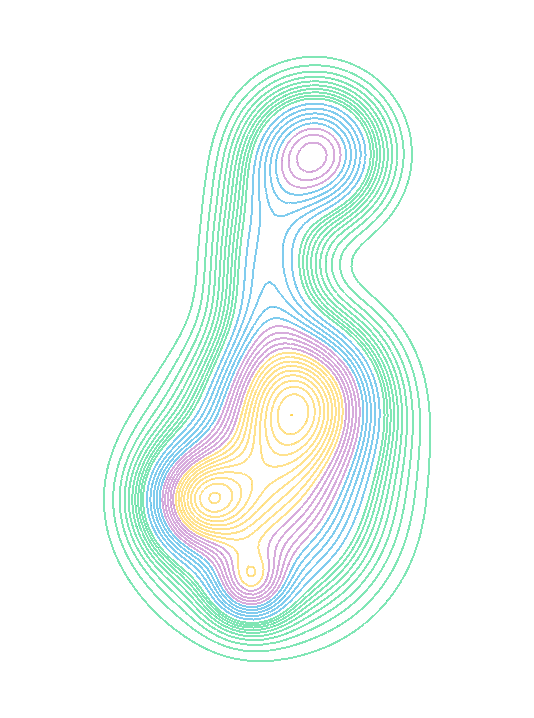
\includegraphics[trim=100 25 75 0, clip, angle=280, scale=0.25]{scripts/figures/scalar_contour.png}
    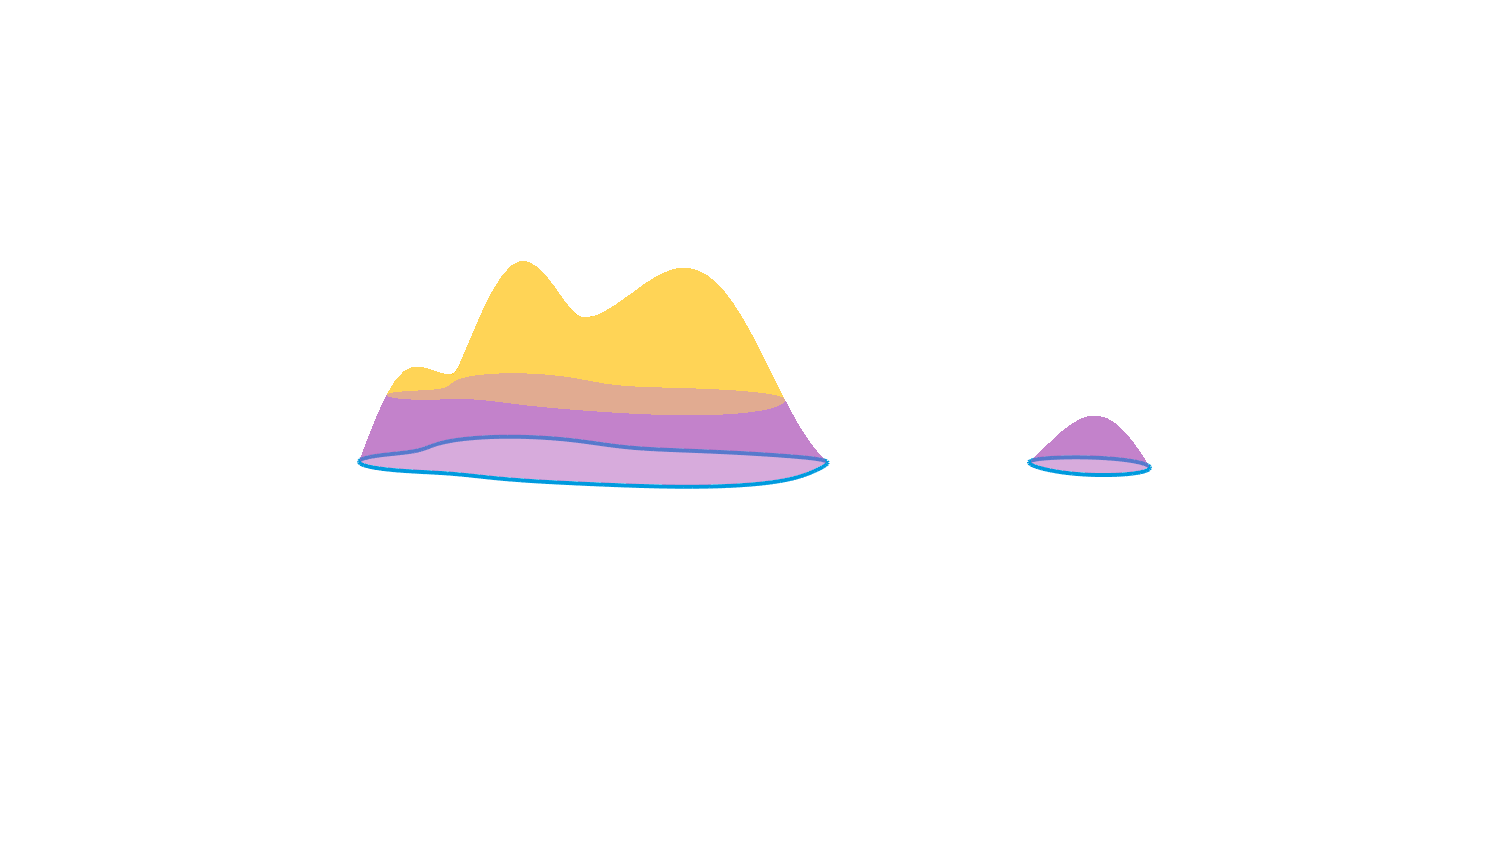
\includegraphics[trim=200 300 200 200, clip, width=0.5\textwidth]{../scripts/figures/surf/ass1_C_side.png}
    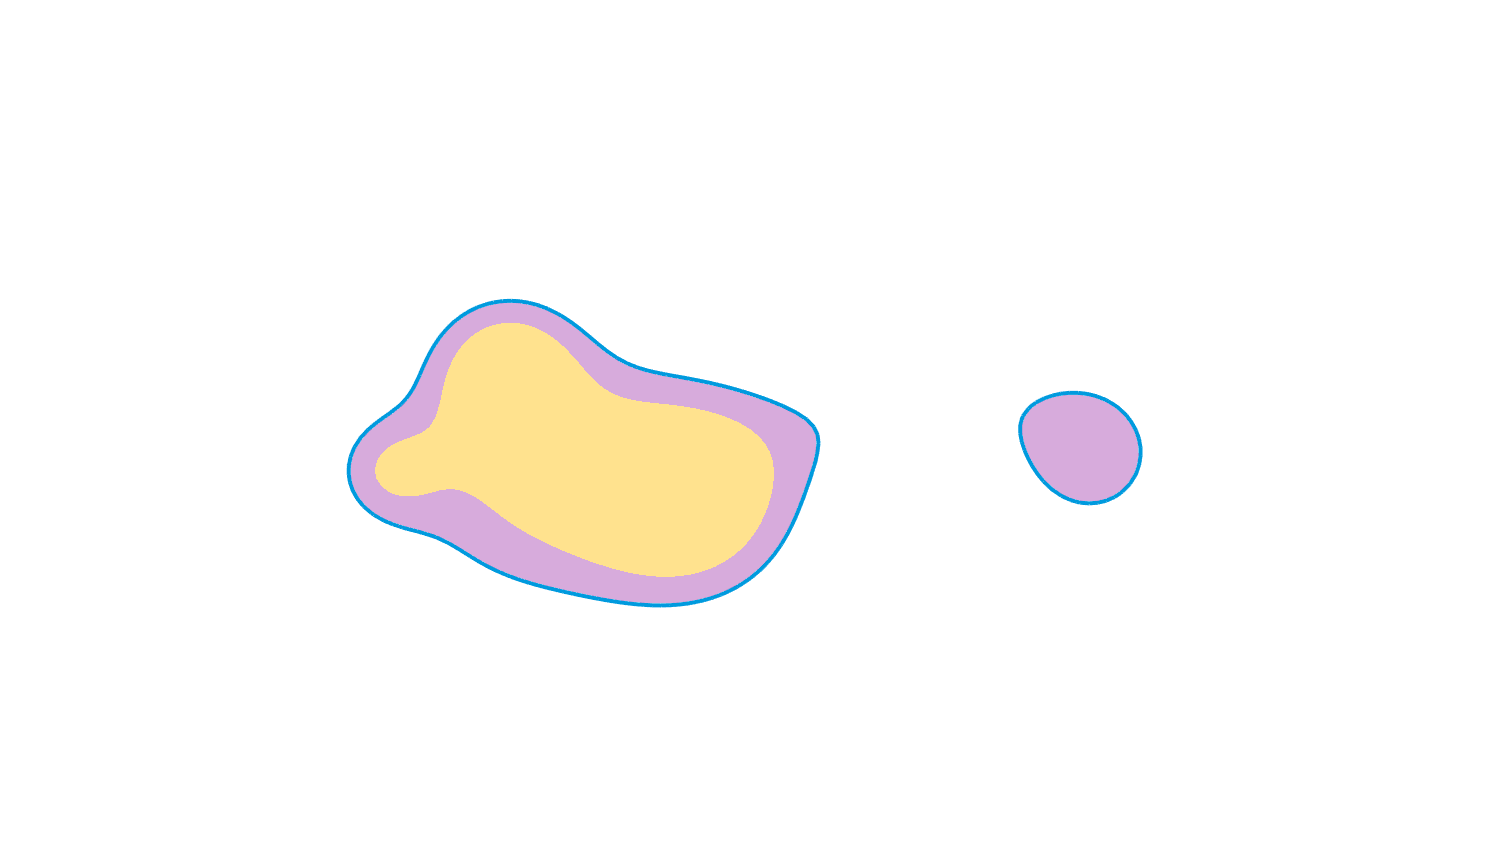
\includegraphics[trim=300 150 200 200, clip, width=0.3\textwidth]{../scripts/figures/surf/ass1_C_top.png}
    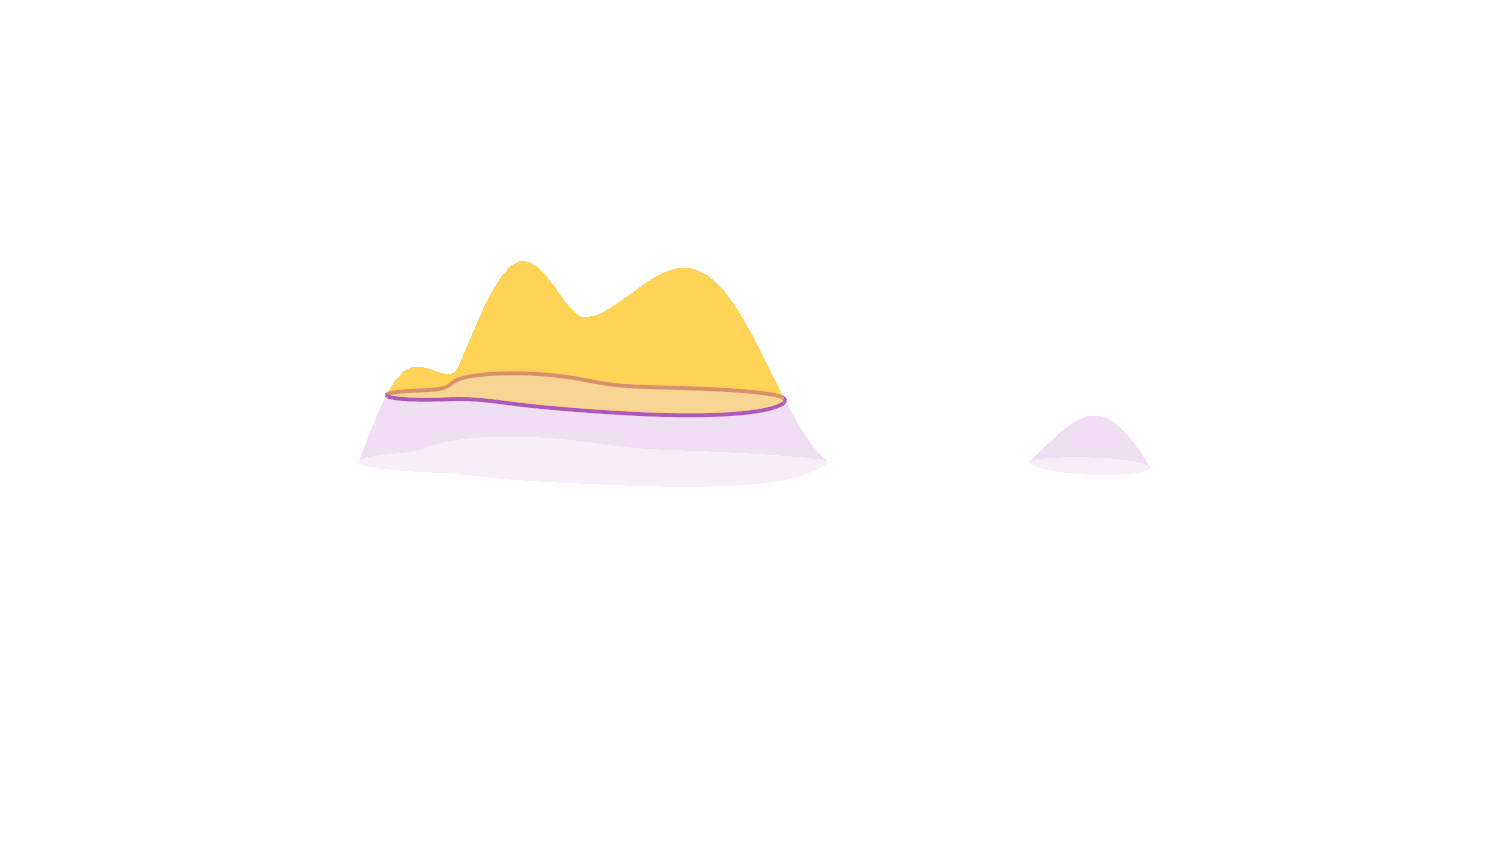
\includegraphics[trim=200 300 200 200, clip, width=0.5\textwidth]{../scripts/figures/surf/ass1_D_side.png}
    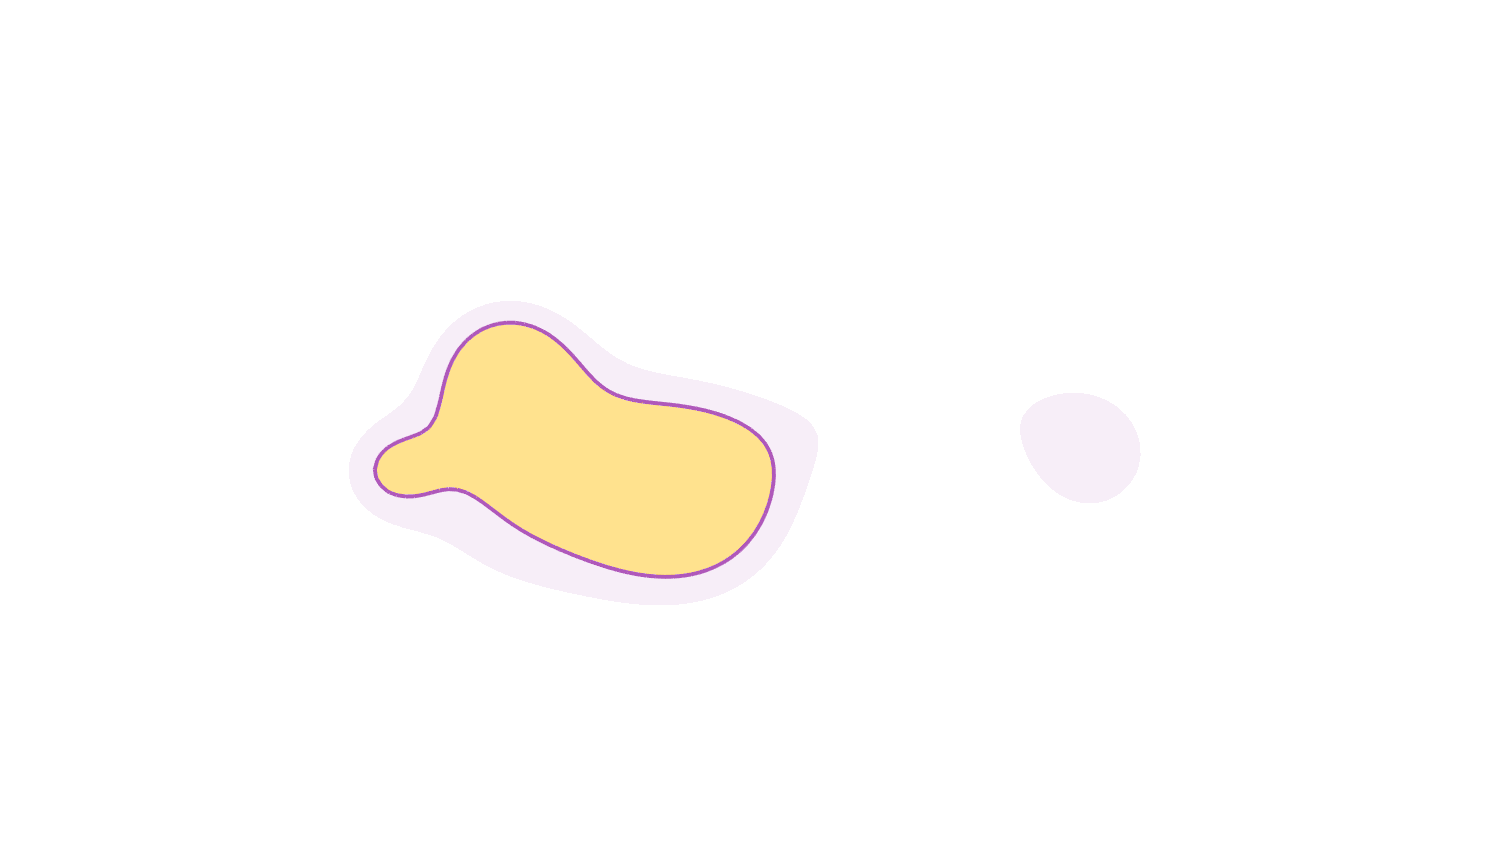
\includegraphics[trim=300 150 200 200, clip, width=0.3\textwidth]{../scripts/figures/surf/ass1_D_top.png}
    % 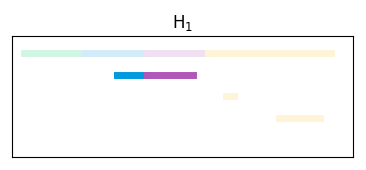
\includegraphics[scale=0.7]{scripts/figures/scalar_barcode_H1-masked.png}
  \end{textblock*}
\end{frame}

\begin{frame}
  \frametitle{{\small Assumption 1 and the Geometric TCC}}

  % \[\begin{tikzcd}
  %   \hom_0(\overline{B_{\omega+c(\delta+\zeta)}},\overline{D})\arrow{d}{m} \arrow{r}{j} &
  %   \hom_0(\overline{B_\omega}, \overline{D}) \arrow{d}{\ell} \\
  %   %
  %   \hom_0(\overline{Q_{\omega+c\delta}^\delta}, \overline{P^\delta}) \arrow{r}{i} &
  %   \hom_0(\overline{Q_{\omega-c\zeta}^\delta}, \overline{P^\delta}).
  % \end{tikzcd}\]

  \begin{theorem}[Geometric TCC]
    % Let $j : \hom_0(\cmp{B_{\omega+c(\delta+\zeta)}},\cmp{D})\to \hom_0(\cmp{\B},\cmp{D})$ and $i : \hom_0(\cmp{\QQ^\of}, \cmp{P^\of})\to \hom_0(\cmp{\Q^\of}, \cmp{P^\of})$ be induced by inclusion.
    %
    If $j$ is surjective and $\mathbf{rk}~i\geq \mathbf{rk}~j$ then $D\setminus B_\omega\subseteq P^\delta$ and $Q_{\omega-c\zeta}^\delta$ surrounds $P^\delta$ in $D$.
  \end{theorem}
\end{frame}

\begin{frame}
  \frametitle{{\small Duality, Assumption 2, and the Algorithmic TCC}}

  % \begin{itemize}
  %   \item Can't compute homology of complements: duality
  %   \item don't know number of connected components: assumption 2
  %   \item Rips-\v Cech interleaving and the Algorithmic TCC
  % \end{itemize}

  \textbf{Duality:} $\hom_d(P^\e,Q_z^\e)\cong\hom_0(D\setminus Q_z^\e, D\setminus P^\e)$.

  % \begin{textblock*}{12cm}(1cm,4.5cm)
  %
  % \end{textblock*}
\end{frame}


\begin{frame}
  \frametitle{{\small Duality, Assumption 2, and the Algorithmic TCC}}

  % \begin{itemize}
  %   \item Can't compute homology of complements: duality
  %   \item don't know number of connected components: assumption 2
  %   \item Rips-\v Cech interleaving and the Algorithmic TCC
  % \end{itemize}

  \only<1>{\begin{textblock*}{11cm}(1cm,2cm)
    \textbf{Assumption 2:} $\hom_0(D\setminus B_\omega\hookrightarrow D\setminus B_{\omega-c(\delta+\zeta)})$ is \emph{injective}.
  \end{textblock*}}

  \begin{textblock*}{12cm}(1cm,4.5cm)
    \includegraphics<1>[trim=200 300 200 200, clip, width=0.5\textwidth]{../scripts/figures/surf/ass2_C_side.png}
    \includegraphics<1>[trim=300 200 200 200, clip, width=0.3\textwidth]{../scripts/figures/surf/ass2_C_top.png}
    \includegraphics<1>[trim=200 300 200 200, clip, width=0.5\textwidth]{../scripts/figures/surf/ass2_B_side.png}
    \includegraphics<1>[trim=300 200 200 200, clip, width=0.3\textwidth]{../scripts/figures/surf/ass2_B_top.png}
  \end{textblock*}

  \only<2>{\begin{lemma}\label{lem:assumption2}
    If $\hom_0(D\setminus B_\omega\hookrightarrow D\setminus B_{\omega+c(\delta+\zeta)})$ is injective and each component of $D\setminus B_\omega$ contains a point in $P$ then $\mathbf{dim}~\hom_0(\rips^\delta(P\setminus Q_{\omega-c\zeta})) \geq \mathbf{dim}~\hom_0(D\setminus B_\omega)$.
  \end{lemma}}
\end{frame}

\begin{frame}
  \frametitle{{\small Duality, Assumption 2, and the Algorithmic TCC}}

  % \begin{itemize}
  %   \item Can't compute homology of complements: duality
  %   \item don't know number of connected components: assumption 2
  %   \item Rips-\v Cech interleaving and the Algorithmic TCC
  % \end{itemize}
  \begin{small}
    \[ \hom_k(\rips^\e(P, Q_w))\xrightarrow{J_w^\e}\hom_k(\cech^\e(P, Q_w))\xrightarrow{I_w^\e}\hom_k(\rips^\e(P, Q_w))\]
    % so
    % \[\mathbf{rk}~\hom_d(\cech^{\delta}(P, Q_{\omega-c\zeta})\hookrightarrow\cech^{\delta}(P, Q_{\omega+c\delta})) \geq\mathbf{rk}~ \hom_d(\rips^{\delta}(P, Q_{\omega-c\zeta})\hookrightarrow\rips^{2\delta}(P, Q_{\omega+c\delta}))\]

    \begin{theorem}[Algorithmic TCC]\label{thm:algo_tcc}
      Suppose $\hom_0(D\setminus B_{\omega+c(\delta+\zeta)}\hookrightarrow D\setminus B_\omega)$ is surjective and $\hom_0(D\setminus B_\omega\hookrightarrow D\setminus B_{\omega-c(\delta+\zeta)})$ is injective.

       If $\mathbf{rk}~\hom_d(\rips^\delta(P, Q_{\omega -c\zeta})\hookrightarrow \rips^{2\delta}(P, Q_{\omega+c\delta})) \geq \mathbf{dim}~\hom_0(\rips^\delta(P\setminus Q_{\omega-c\zeta}))$ then $D\setminus B_\omega\subseteq P^\delta$ and $Q_{\omega-c\zeta}^\delta$ surrounds $P^\delta$ in $D$.
    \end{theorem}
  \end{small}

  % \begin{textblock*}{12cm}(1cm,4.5cm)
  %
  % \end{textblock*}
\end{frame}

  % % \input{excision}
  % \input{stability}
  % \input{sampling}
  % % \input{extension}
  % \clearpage
  %
  % \section{Experiments}\label{sec:experiments}
  % \input{software}
  % % !TeX root = ../../main.tex

In this section we will discuss a number of experiments that illustrate the benefit of truncated diagrams, and their approximation by relative diagrams, in comparison to their restricted counterparts.
We will focus on the persistent homology of functions on a square 2D grid---that is, functions with non-trivial persistent homology in dimensions zero and one.
While these experiments can be conducted in dimension zero or one we will focus on $\hom_1$.
We chose as our function a radially symmetric damped sinusoid with random noise, depicted in Figure~\ref{fig:ripple1}, as it has prominent persistent homology in dimension one.

\paragraph*{Experimental setup.}

\begin{figure}[htbp]
  \centering
  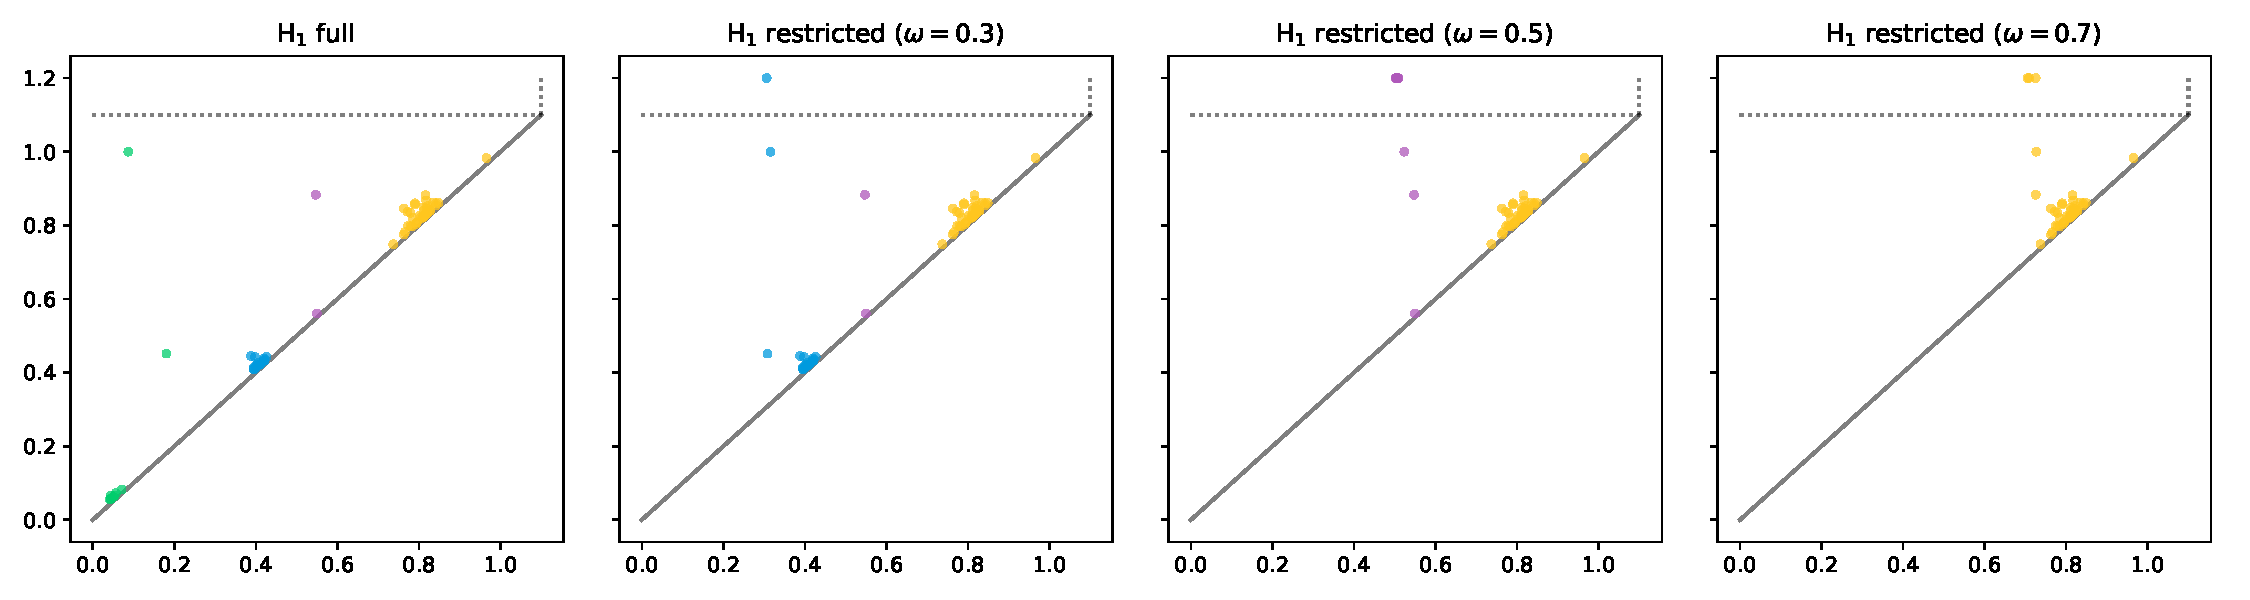
\includegraphics[trim=0 0 790 0, clip, width=0.3\textwidth]{figures/matching-full-dgm.pdf}
  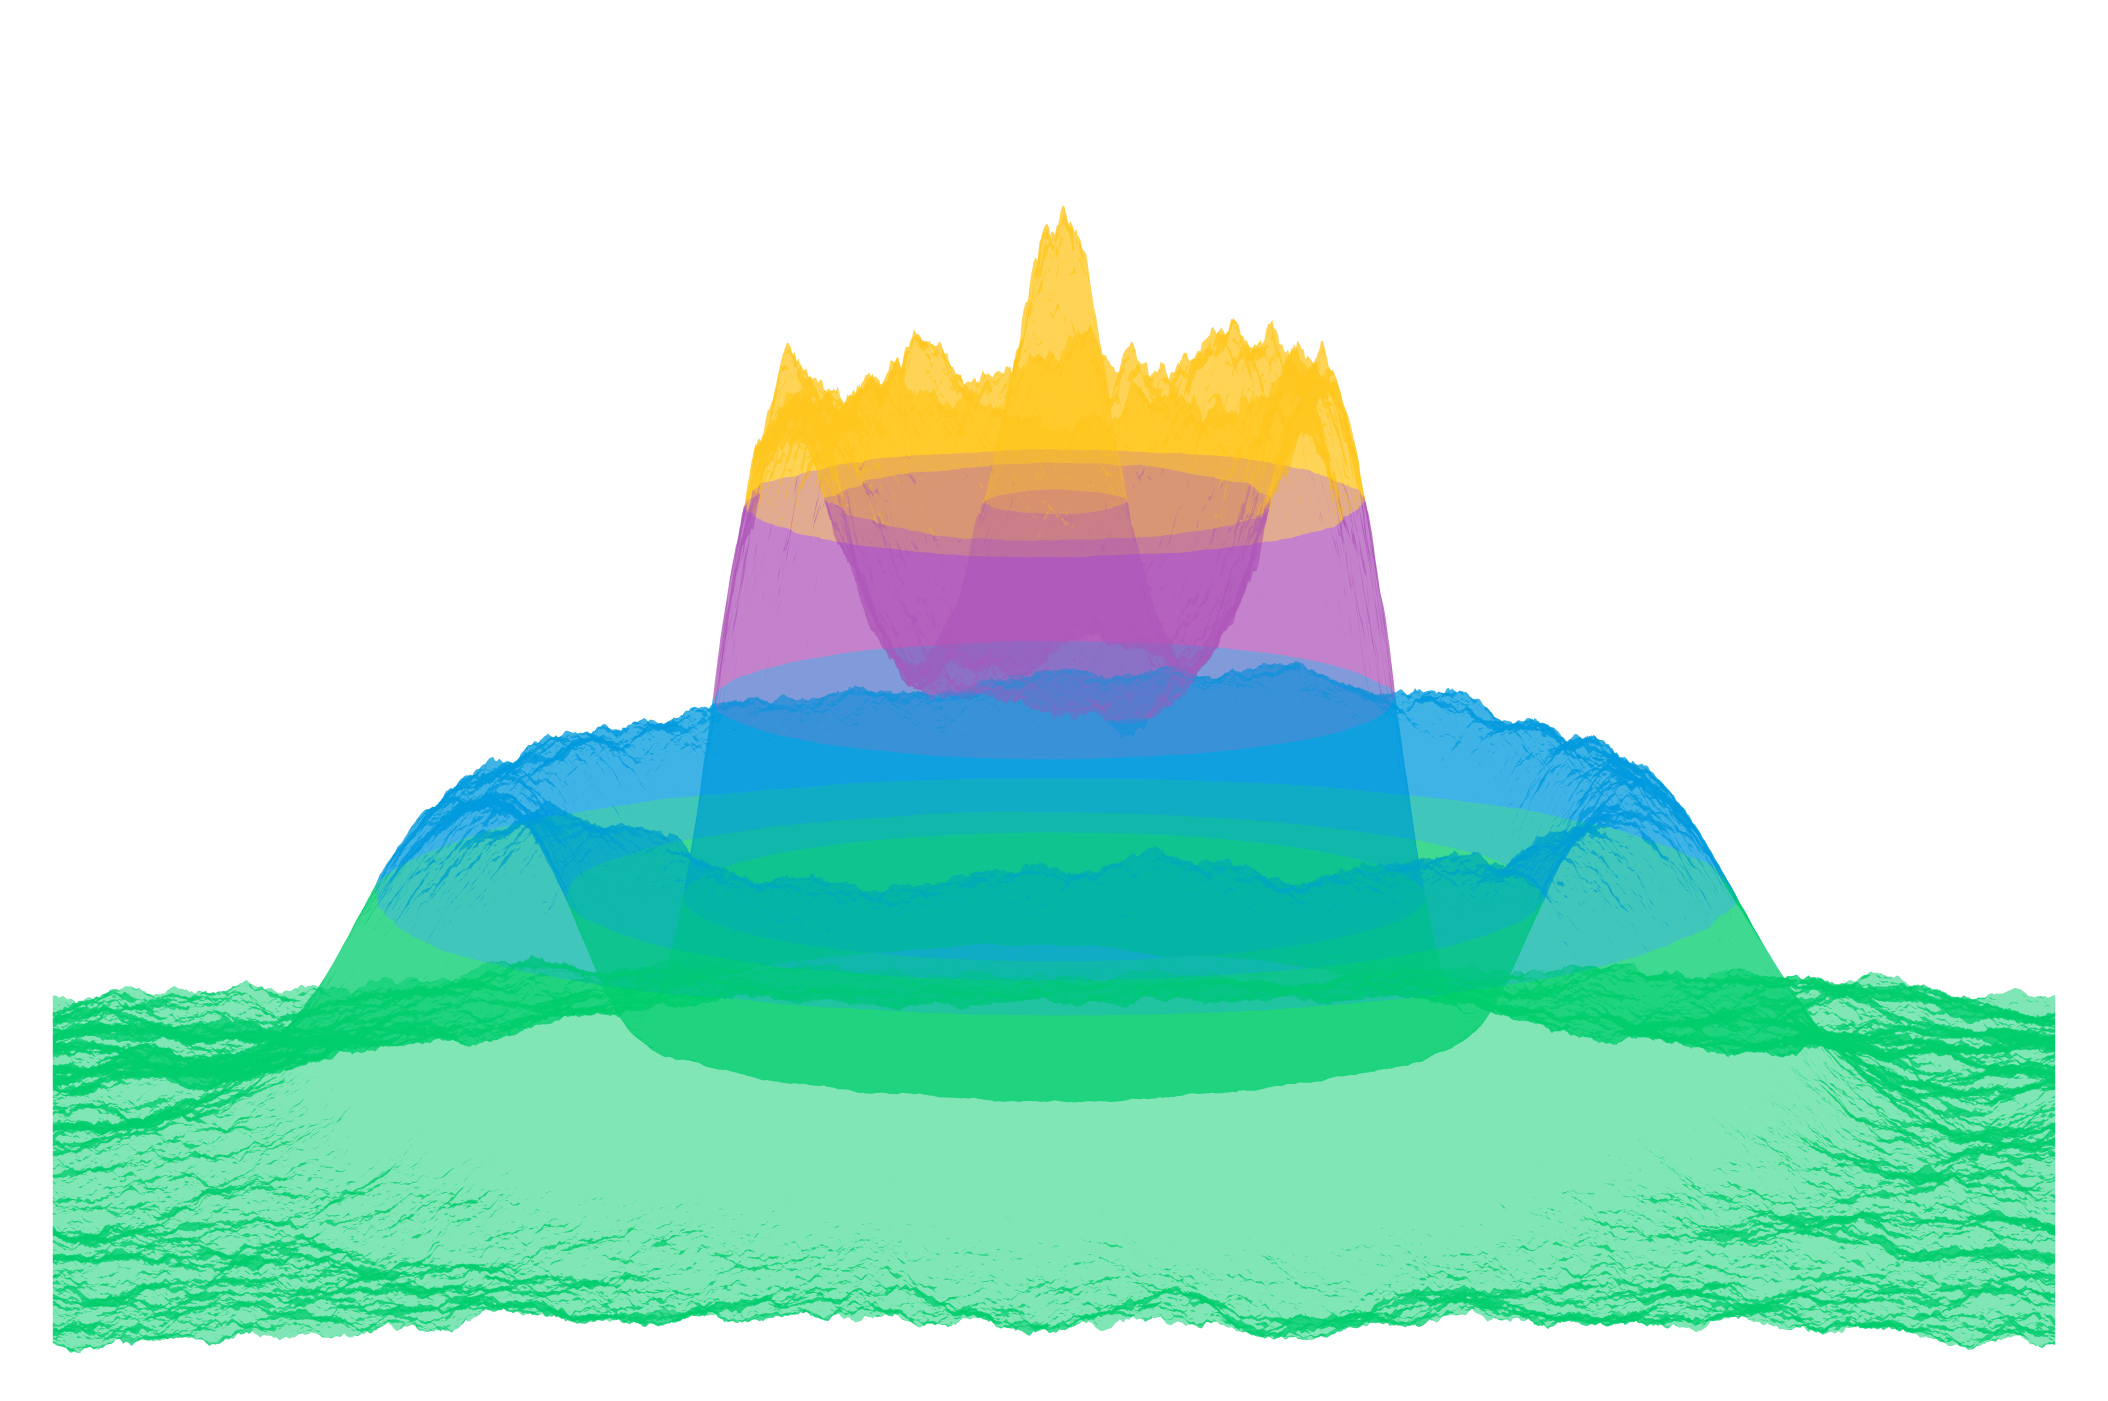
\includegraphics[trim=-350 -800 -700 -300, clip, width=0.4\textwidth]{figures/matching-full-surf_side-lowres.png}
  
\includegraphics[trim=0 -800 0 0, width=0.25\textwidth]{figures/matching-full-surf_top-lowres.png}
  % \includegraphics[trim=0 0 0 -10, clip, width=\textwidth]{scripts/figures/matching1/817_1024-3_1-1_1.png}
  \caption{The $\hom_1$ persistence diagram of the sinusoidal function pictured to the right.
  Features are colored by birth time, infinite features are drawn above the dotted line.}\label{fig:ripple1}
\end{figure}

Throughout, the four interlevel sets shown correspond to the ranges $[0, 0.3)$, $[0.3, 0.5)$, $[0.5, 0.7)$, and $[0.7, 1)$, respectively.
Our persistent homology computations were done primarily with Dionysus~\cite{morozov12dionysus} augmented with custom software for computing representative cycles of infinite features.
\footnote{3D figures were made with MayaVi, all other figures were made with Matplotlib.}
The persistent homology of our function was computed with the lower-star filtration of the Freudenthal triangulation on an $N\times N$ grid over $[-1,1]\times[-1,1]\subset\R^2$.
We take this filtration as $\{\rips^{2\delta}(P_\alpha)\}$ where $P$ is the set of grid points and $\delta = \sqrt{2} / N$.

We note that the purpose of these experiments is not to demonstrate the effectiveness of our approximation by Rips complexes, but to demonstrate the relationships between restricted, relative, and truncated diagrams.
Therefore, for simplicity, we will omit the inclusion $\rips^{2\delta}(P_\alpha)\hookrightarrow\rips^{4\delta}(P_\alpha)$ and take the persistent homology of $\{\rips^{2\delta}(P_\alpha)\}$ with sufficiently small $\delta$ as our ground-truth.
However, in order to keep our diagrams clean we show only those features a distance at least $4\delta$ from the diagonal.
Note that these features are \emph{not} removed from the diagram, and considered in all computations.

In the following we will take $N = 1024$, so $\delta\approx 1.4\times 10^{-3}$, as our ground-truth.
Figure~\ref{fig:ripple1} shows the \emph{full diagram} of our function with features colored by birth time.
Therefore, for $\omega = 0.3, 0.5, 0.7$ the \emph{truncated diagram} is obtained by successively removing features in each interlevel set.
Recall the \emph{restricted diagram} is that of the function restricted to the $\omega$ \emph{superlvel} set filtration, and computed with $\{\rips^{2\delta}(P_\alpha\setminus Q_\omega)\}$.
We will compare this restricted diagram with the \emph{relative diagram}, computed as the relative persistent homology of the filtration of pairs $\{\rips^{2\delta}(P_\alpha, Q_\omega)\}$.

\paragraph*{The issue with restricted diagrams.}

In order to get an initial sense of the difference between relative and restricted diagrams we first compare the bottleneck distance of each to the truncated diagram.
As we have shown the relative diagram is equal to the truncated diagram with additional infinite features we will remove all infinite features from the bottleneck computation.
We therefore expect the distance between the relative and truncated diagrams to be zero for $N=1024$.

Figure~\ref{fig:bottleneck} shows the bottleneck distance from the truncated diagram at full resolution ($N = 1024$) to both the relative and restricted diagrams with varying resolution.
Specifically, the function on a $1024\times 1024$ grid is down-sampled to grids ranging from $64\times 64$ to $1024\times 1024$.
We also show the expected bottleneck distance to the true truncated diagram given by the interleaving in Theorem~\ref{thm:interleaving_main_2} in black.

\begin{figure}[htbp]
  \centering
  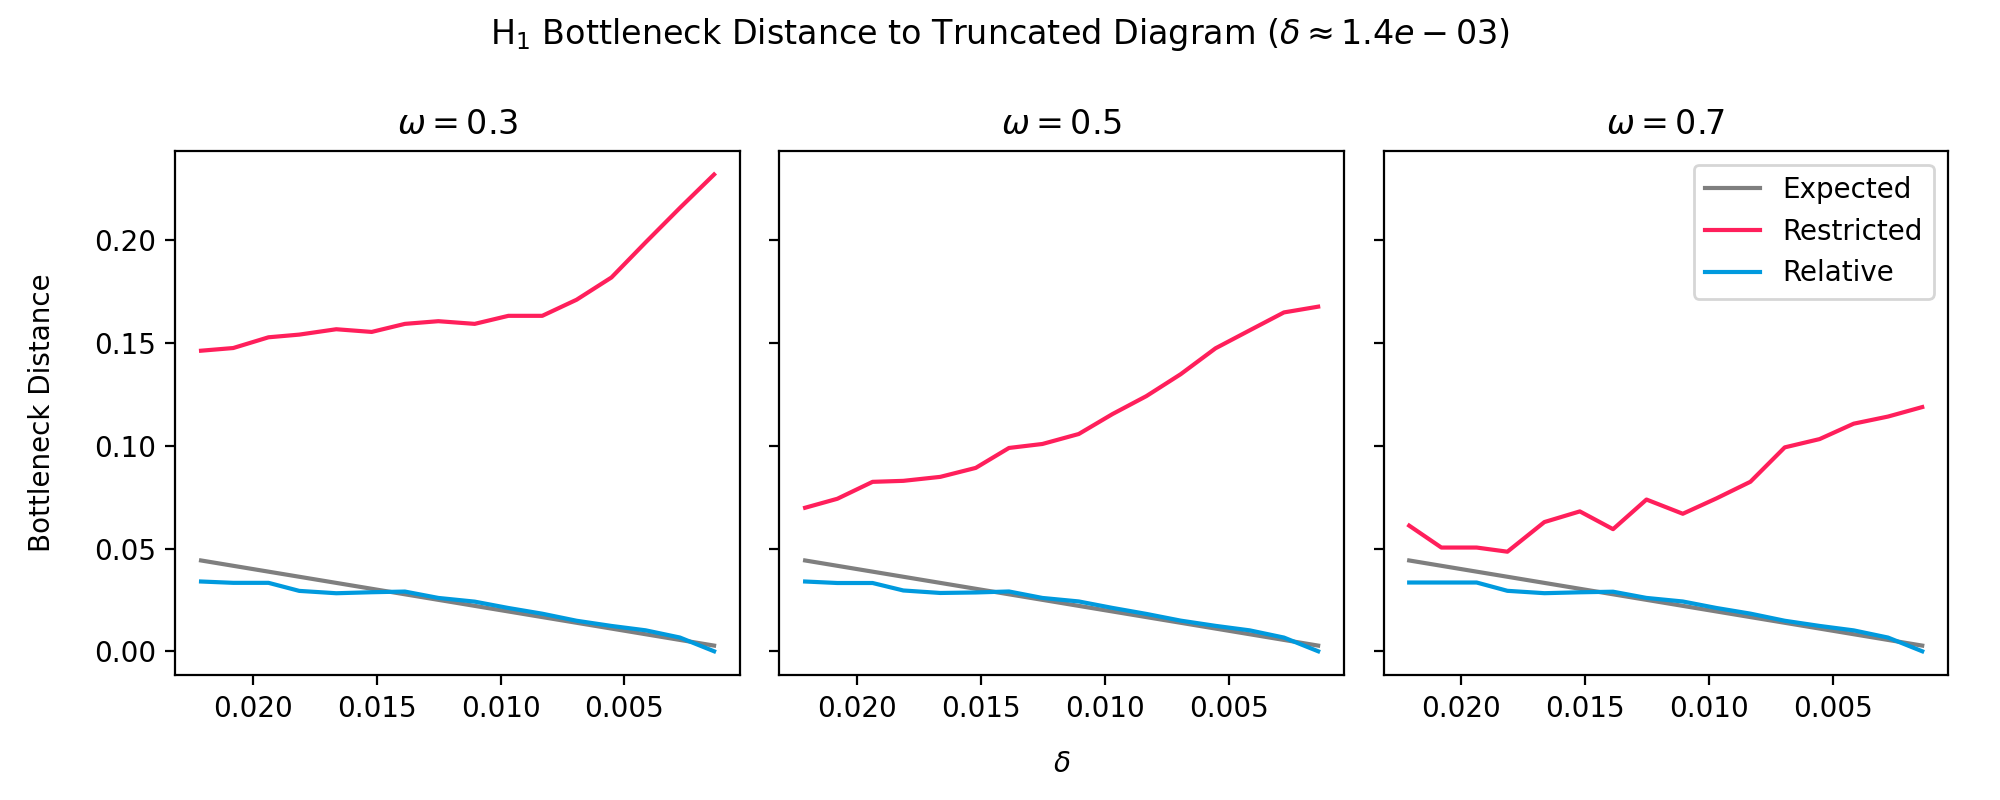
\includegraphics[width=0.95\textwidth]{figures/matching-bottleneck_delta.png}
  \caption{Comparison of the bottleneck distance between the truncated diagram and those of the restricted and relative diagrams with increasing resolution.}\label{fig:bottleneck}
\end{figure}

As we can see, the relative diagram performs better than the restricted diagram, which diverges with increasing resolution.
The reason for this is shown in Figure~\ref{fig:restricted} which depicts the restricted diagrams at $\omega = 0.3, 0.5,$ and $0.7$ at full resolution.
Recall that 1-dimensional features that are born before $\omega$ and die after $\omega$ become infinite 2-dimensional features in the relative diagram, with birth time equal to the death time of the corresponding feature in the full diagram.
These same features remain 1-dimensional figures in the restricted diagram, but with their birth times shifted to $\omega$.
Indeed, the resulting restricted diagram may be closer to the full diagram for sufficiently small $\omega$.
However, the distance will be proportional to the difference between $\omega$ and the true birth time.

\begin{figure}[htbp]
  \centering
  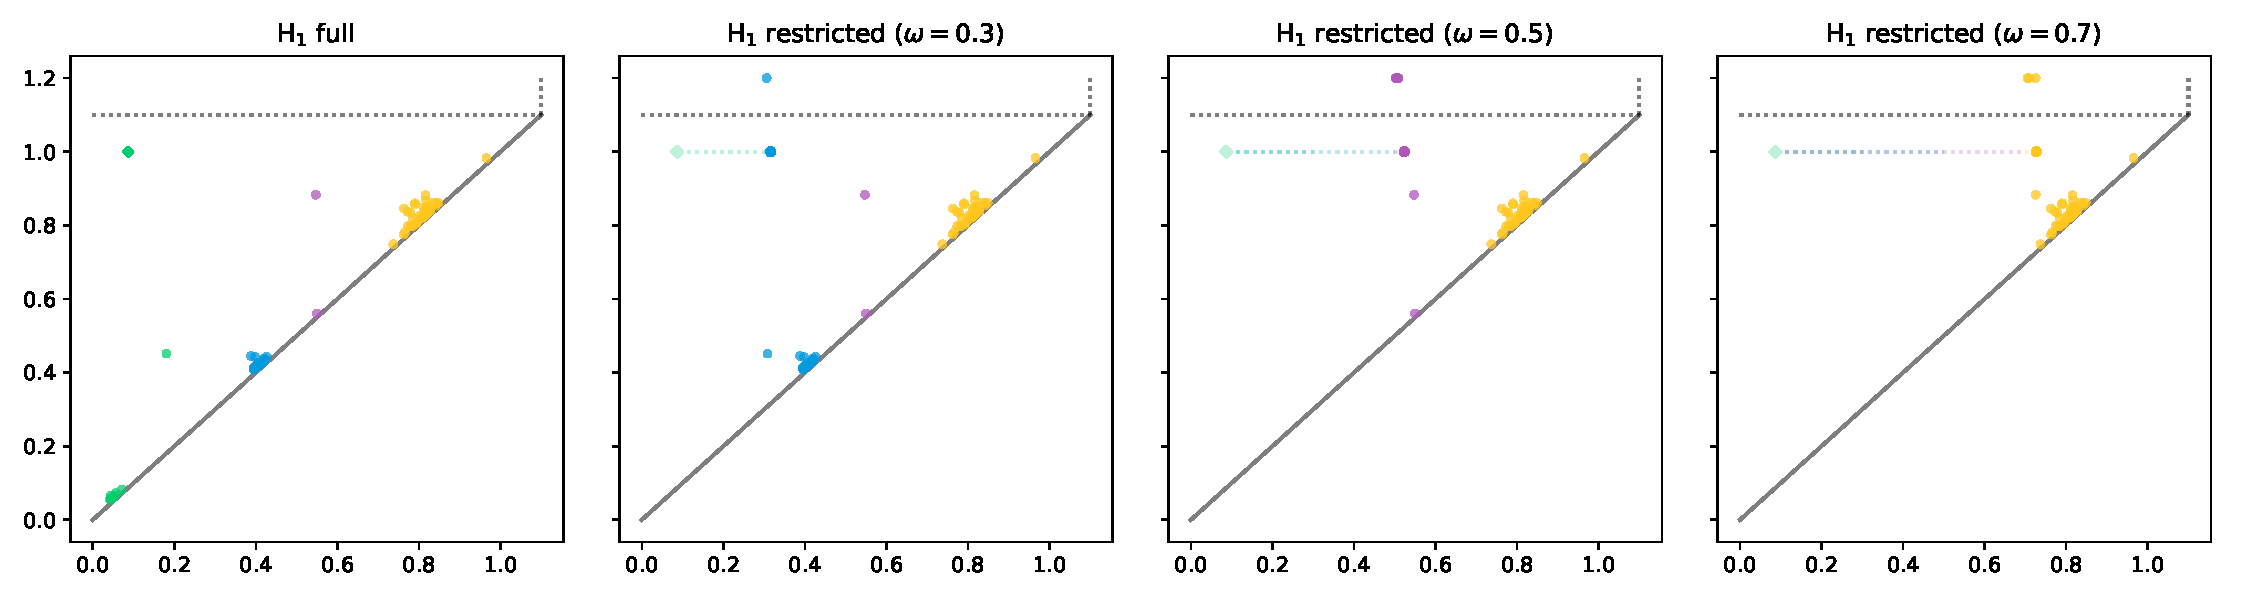
\includegraphics[trim=0 0 -10 0, clip, width=\textwidth]{figures/matching-dgm-1.pdf}
  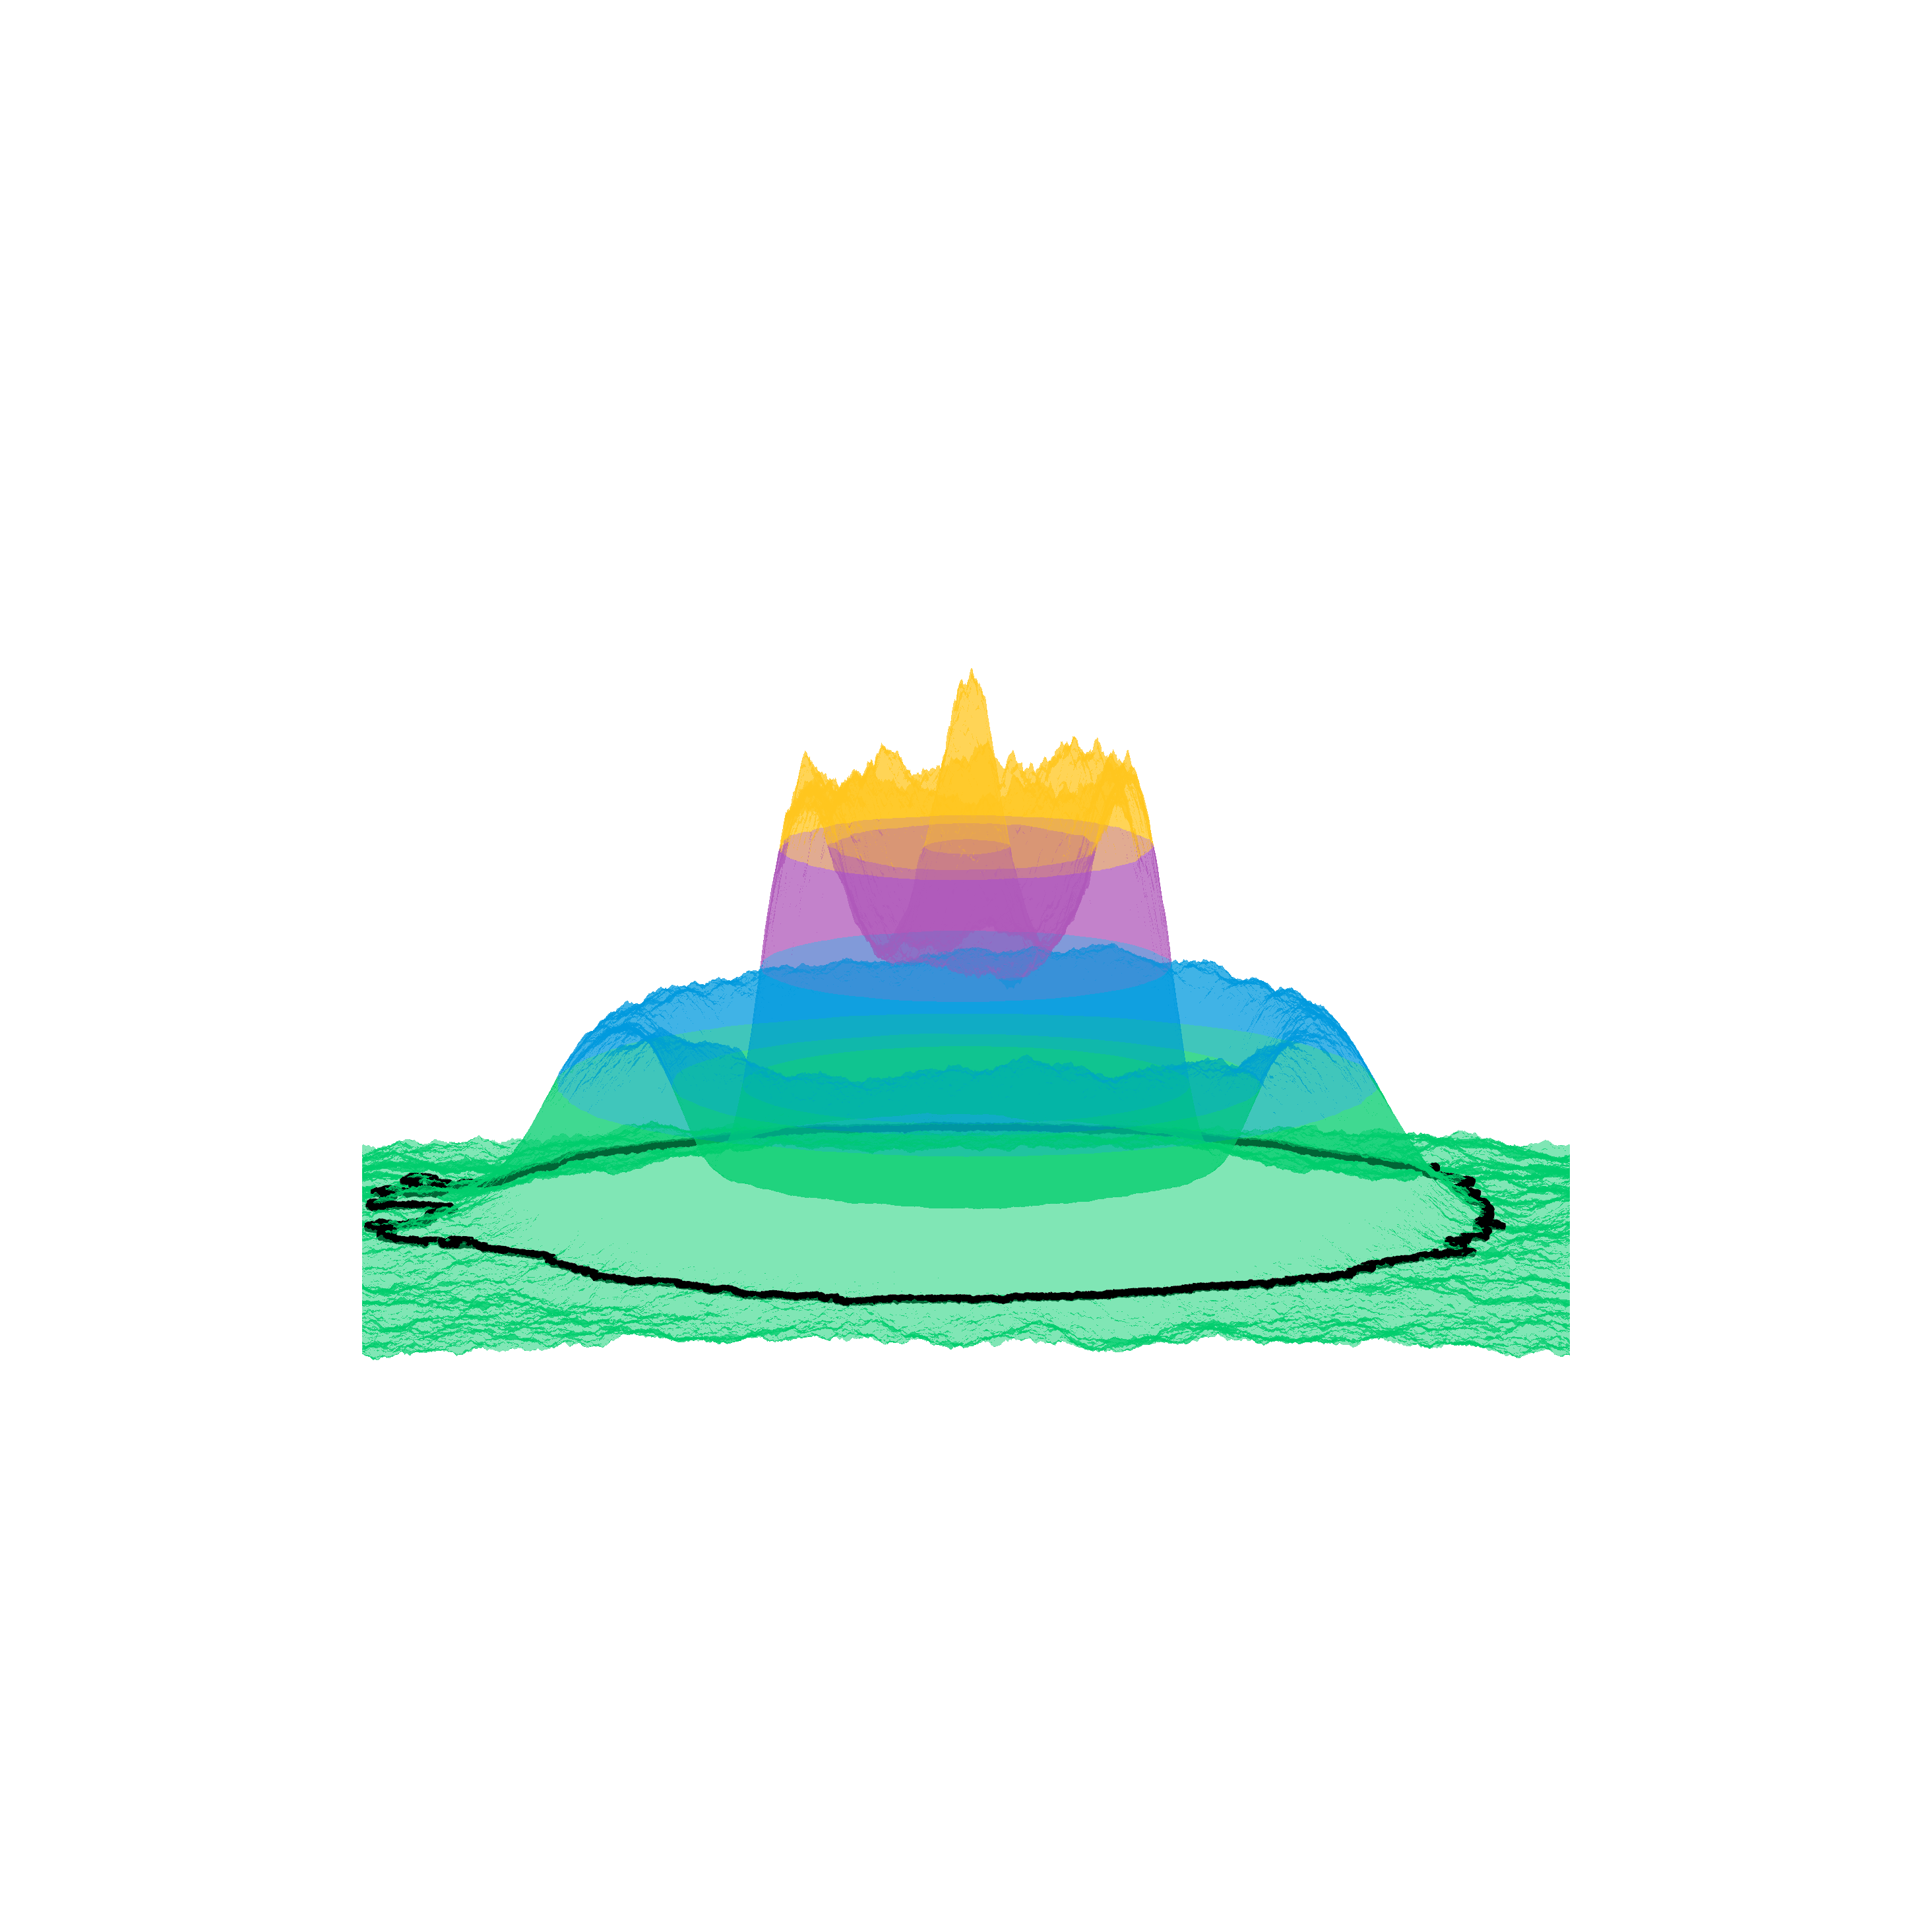
\includegraphics[trim=500 800 500 800, clip, width=0.24\textwidth]{figures/matching-surf_side-1.png}
  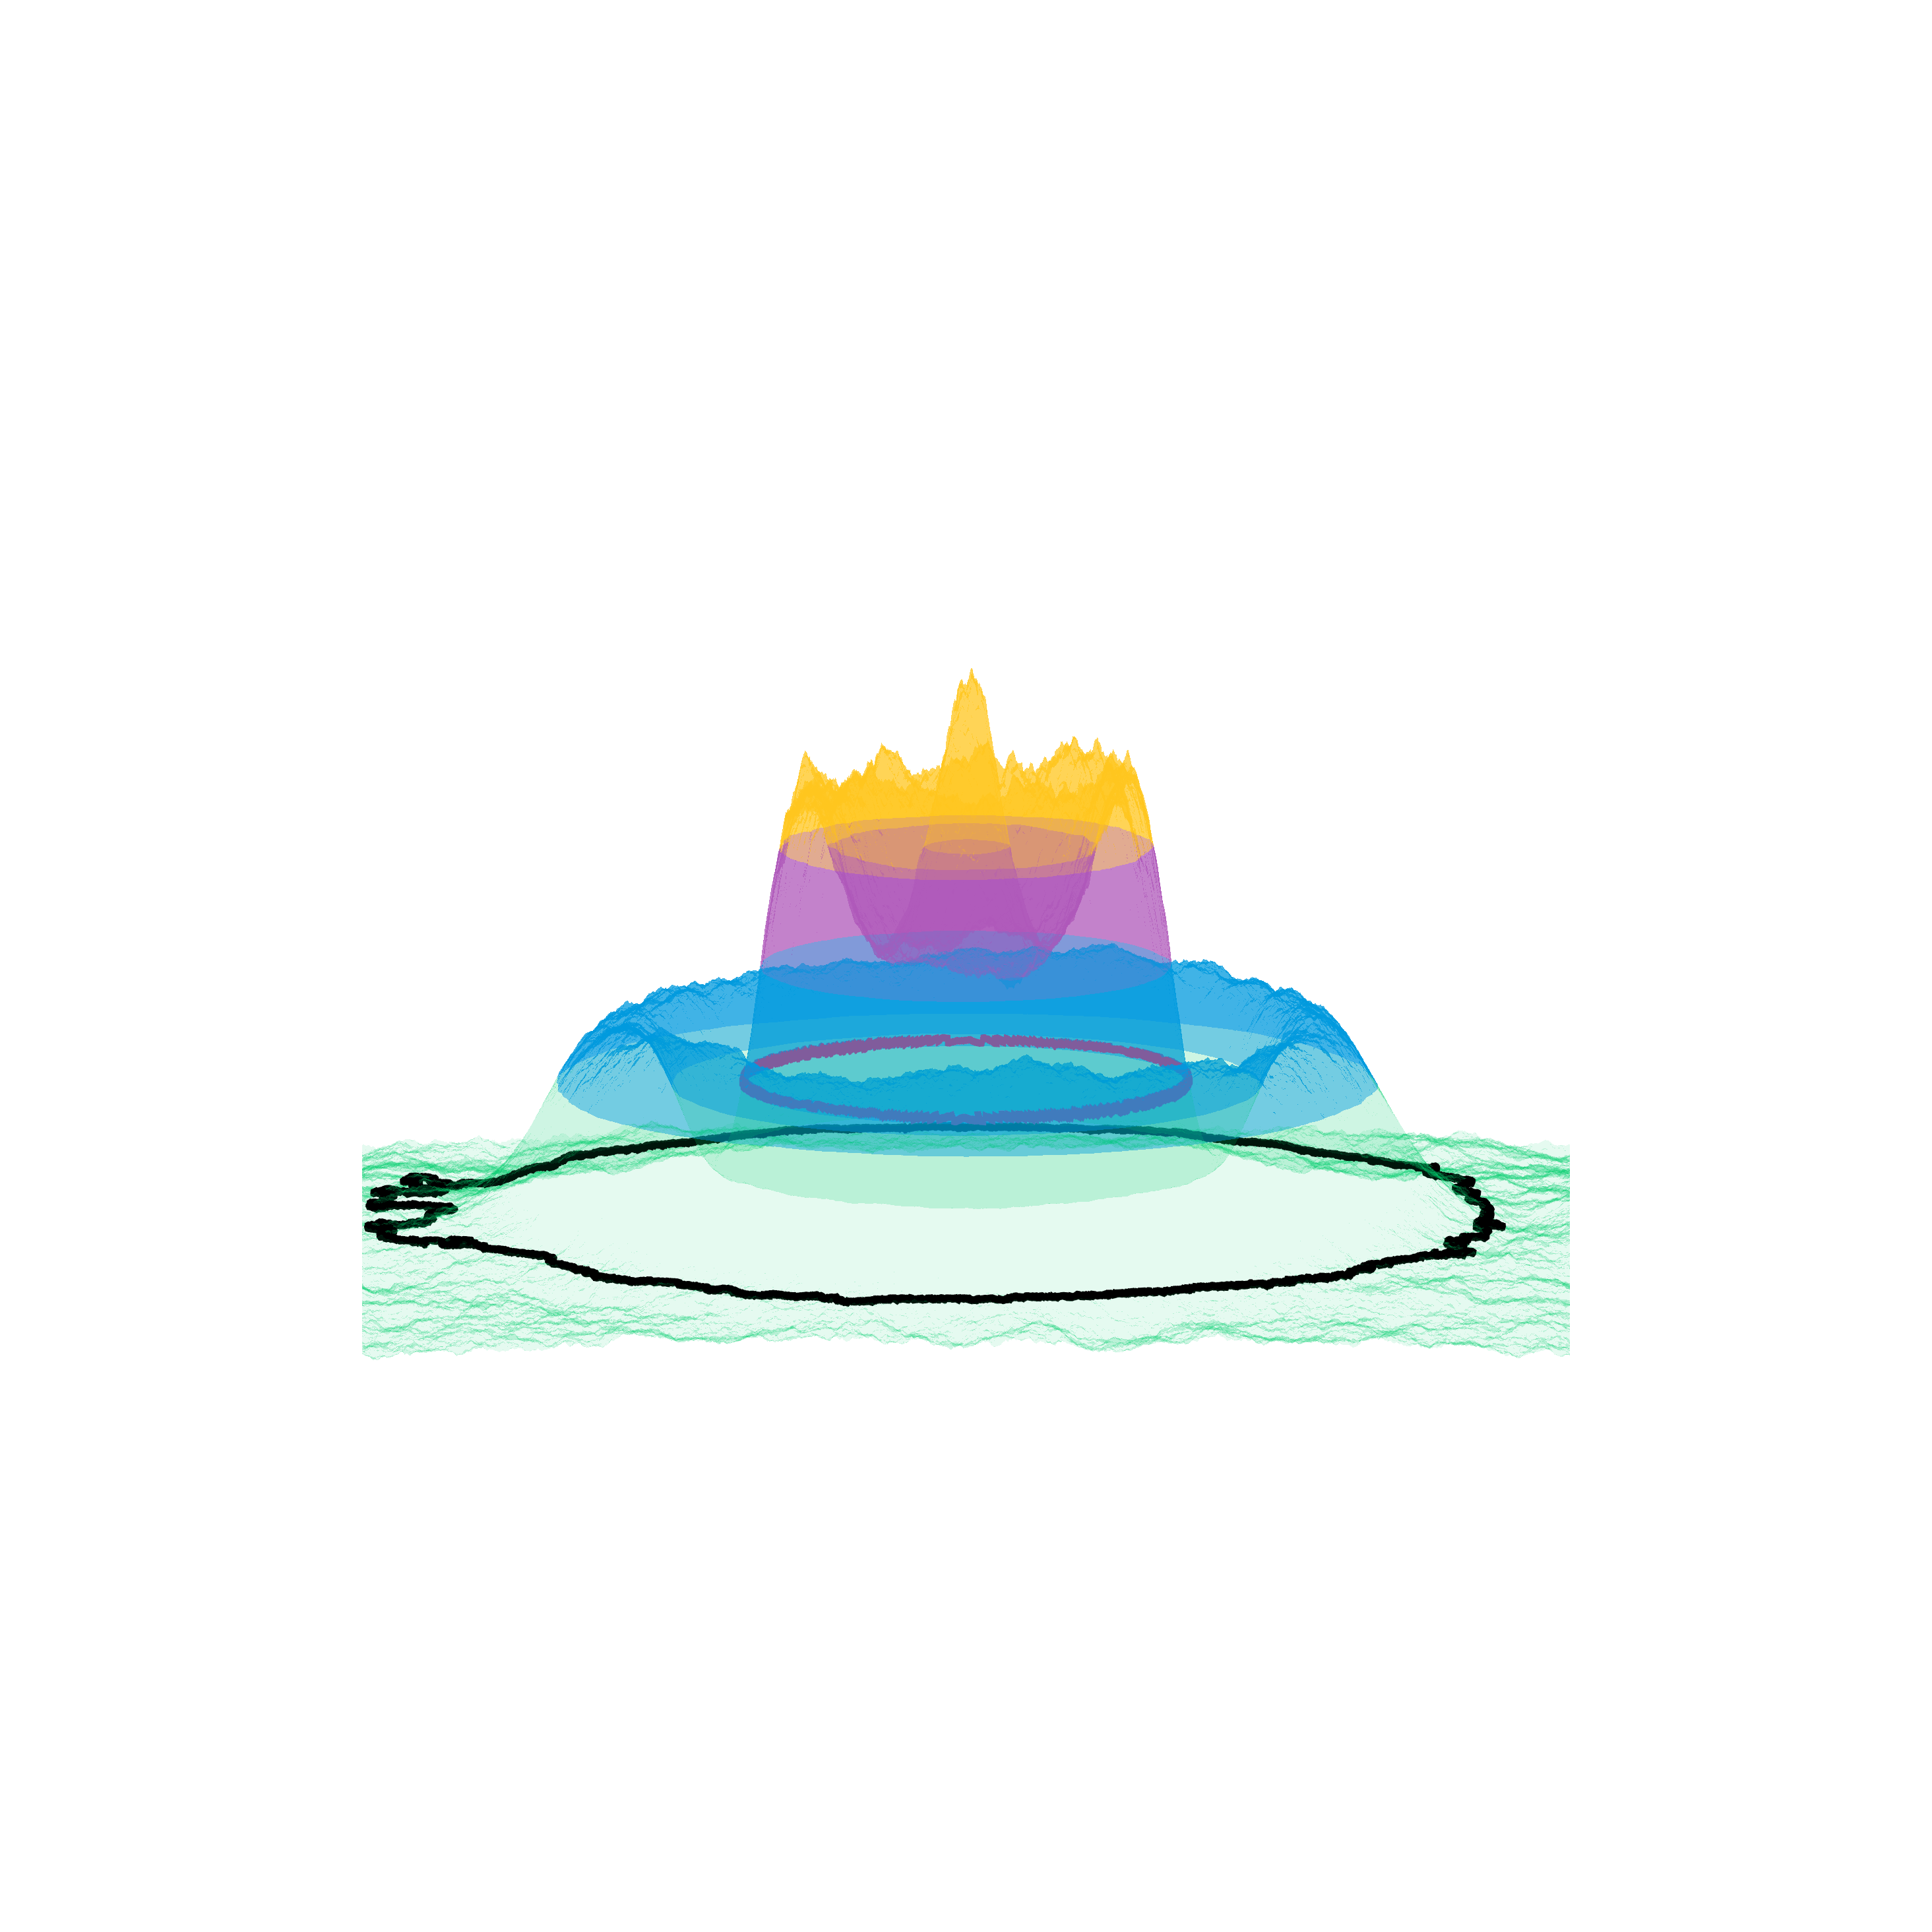
\includegraphics[trim=500 800 500 800, clip, width=0.24\textwidth]{figures/matching-surf_side-1_0.png}
  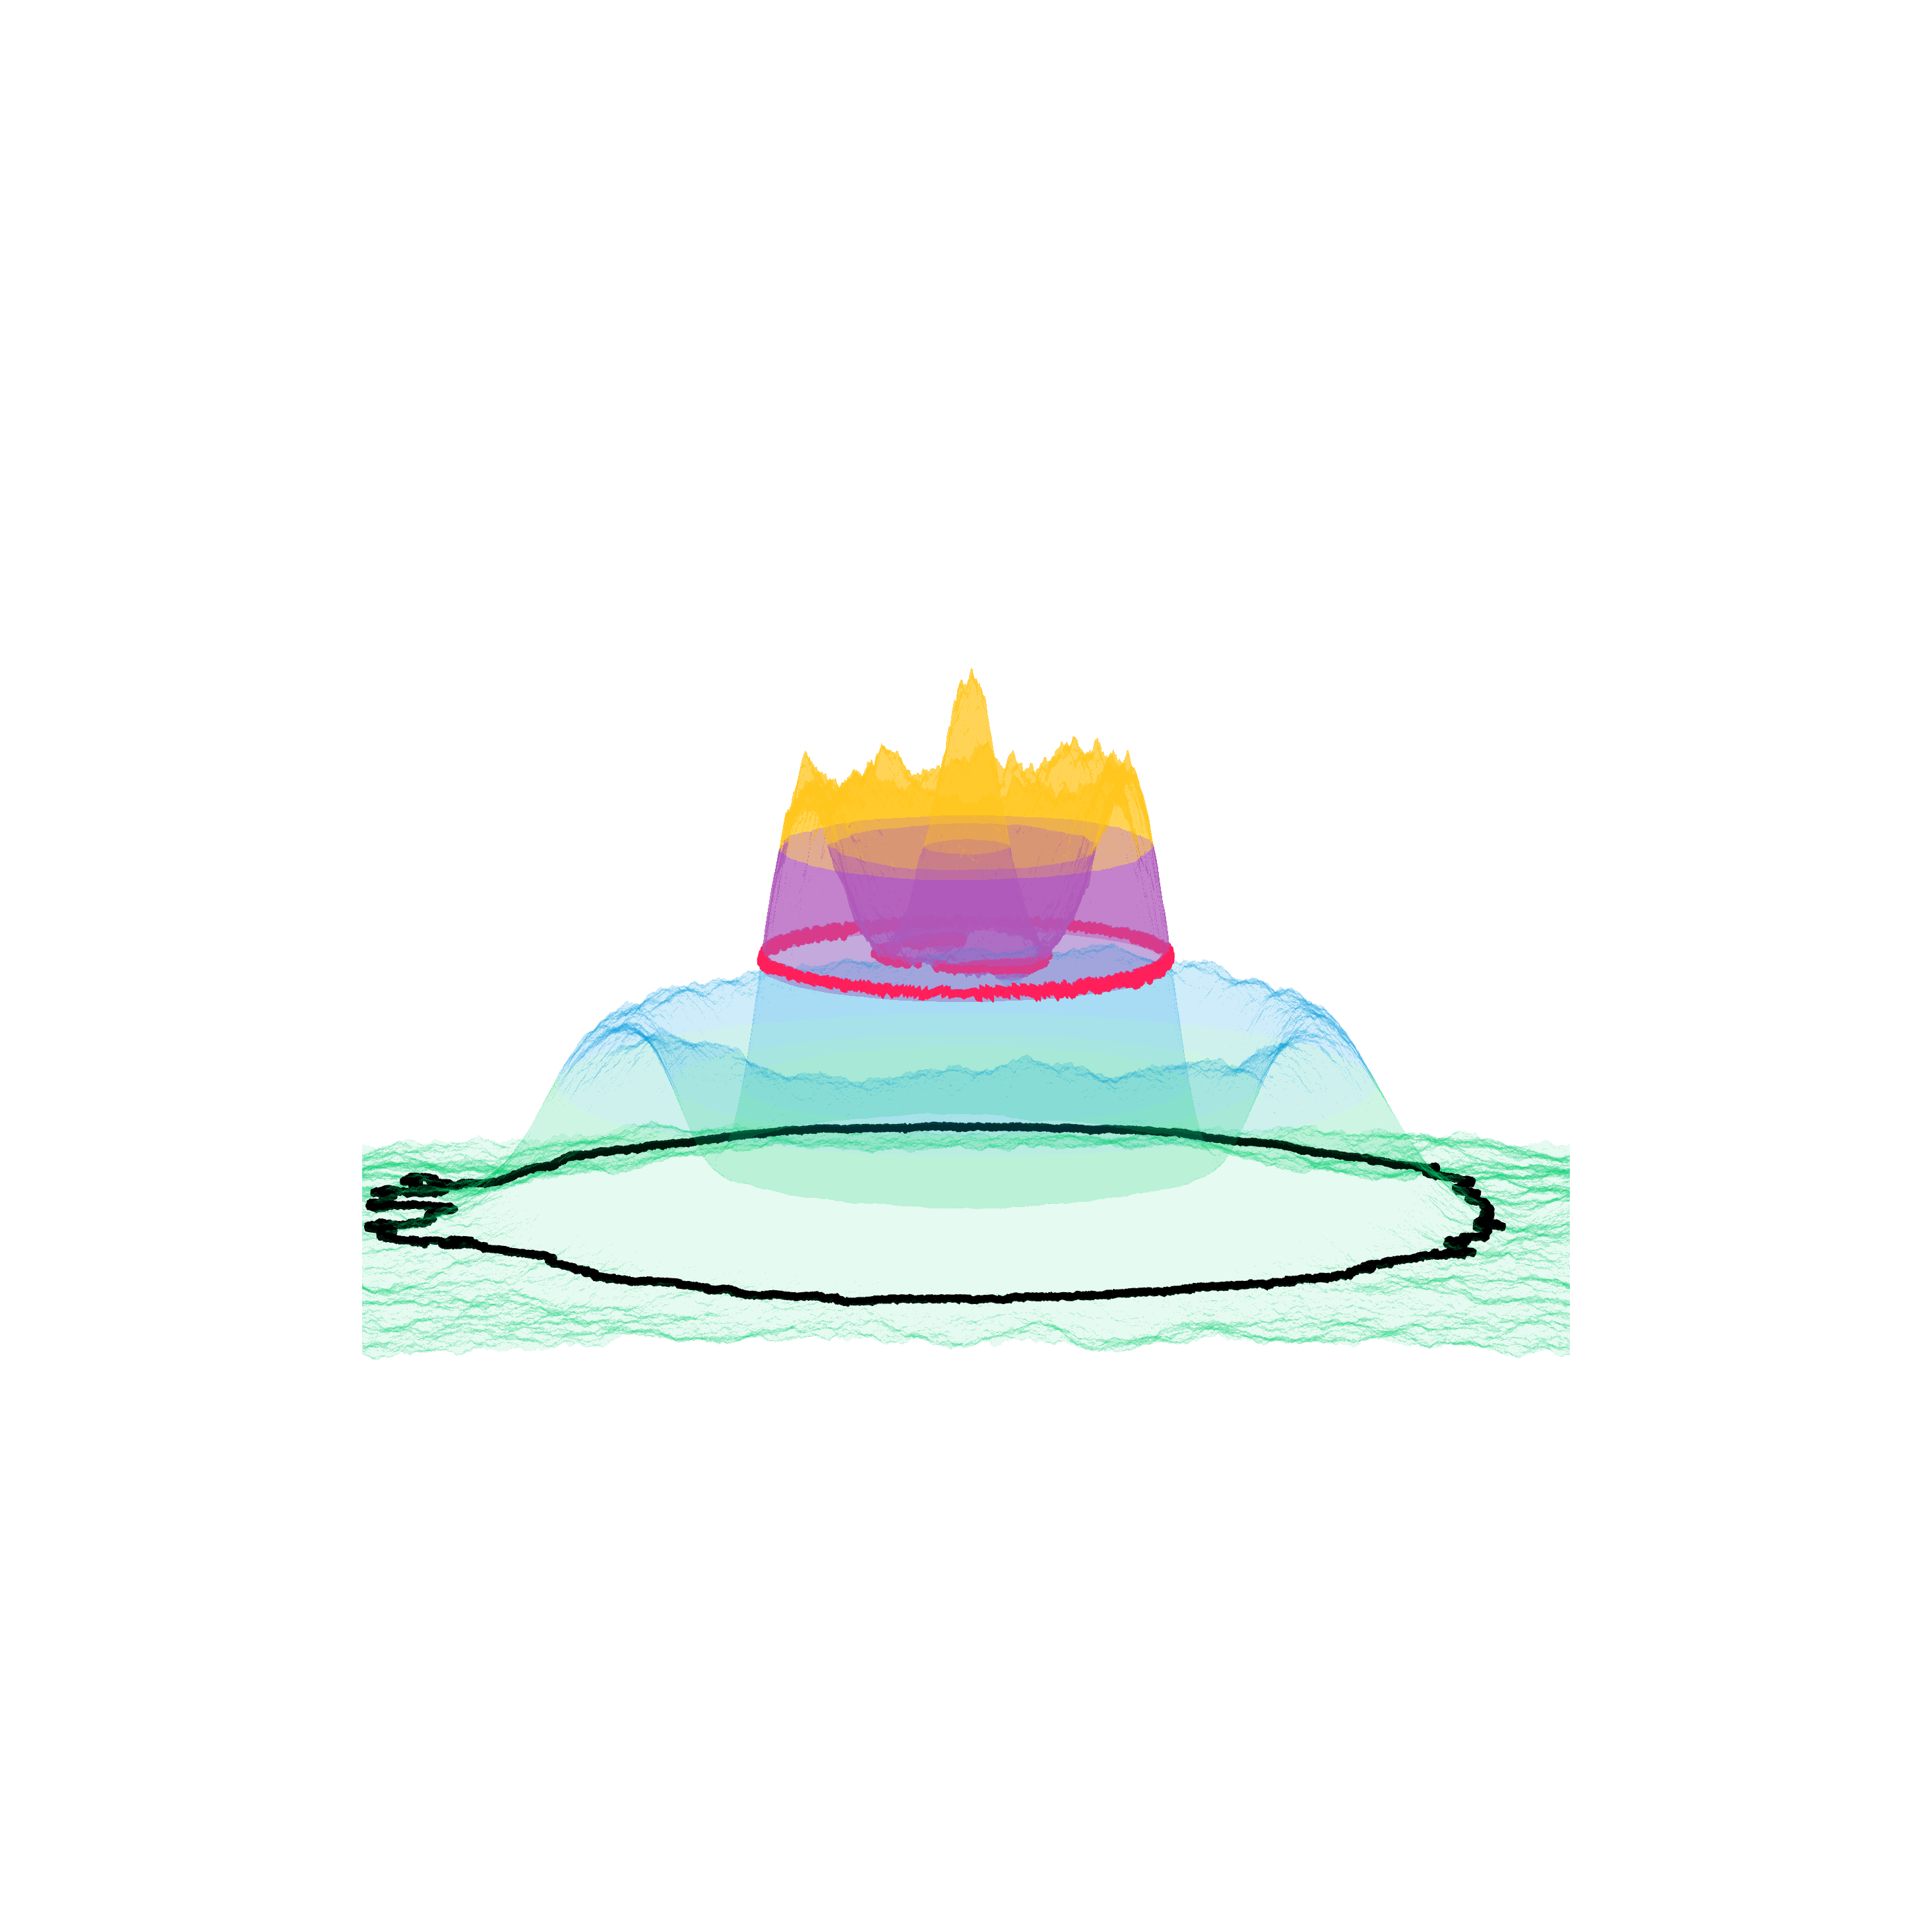
\includegraphics[trim=500 800 500 800, clip, width=0.24\textwidth]{figures/matching-surf_side-1_1.png}
  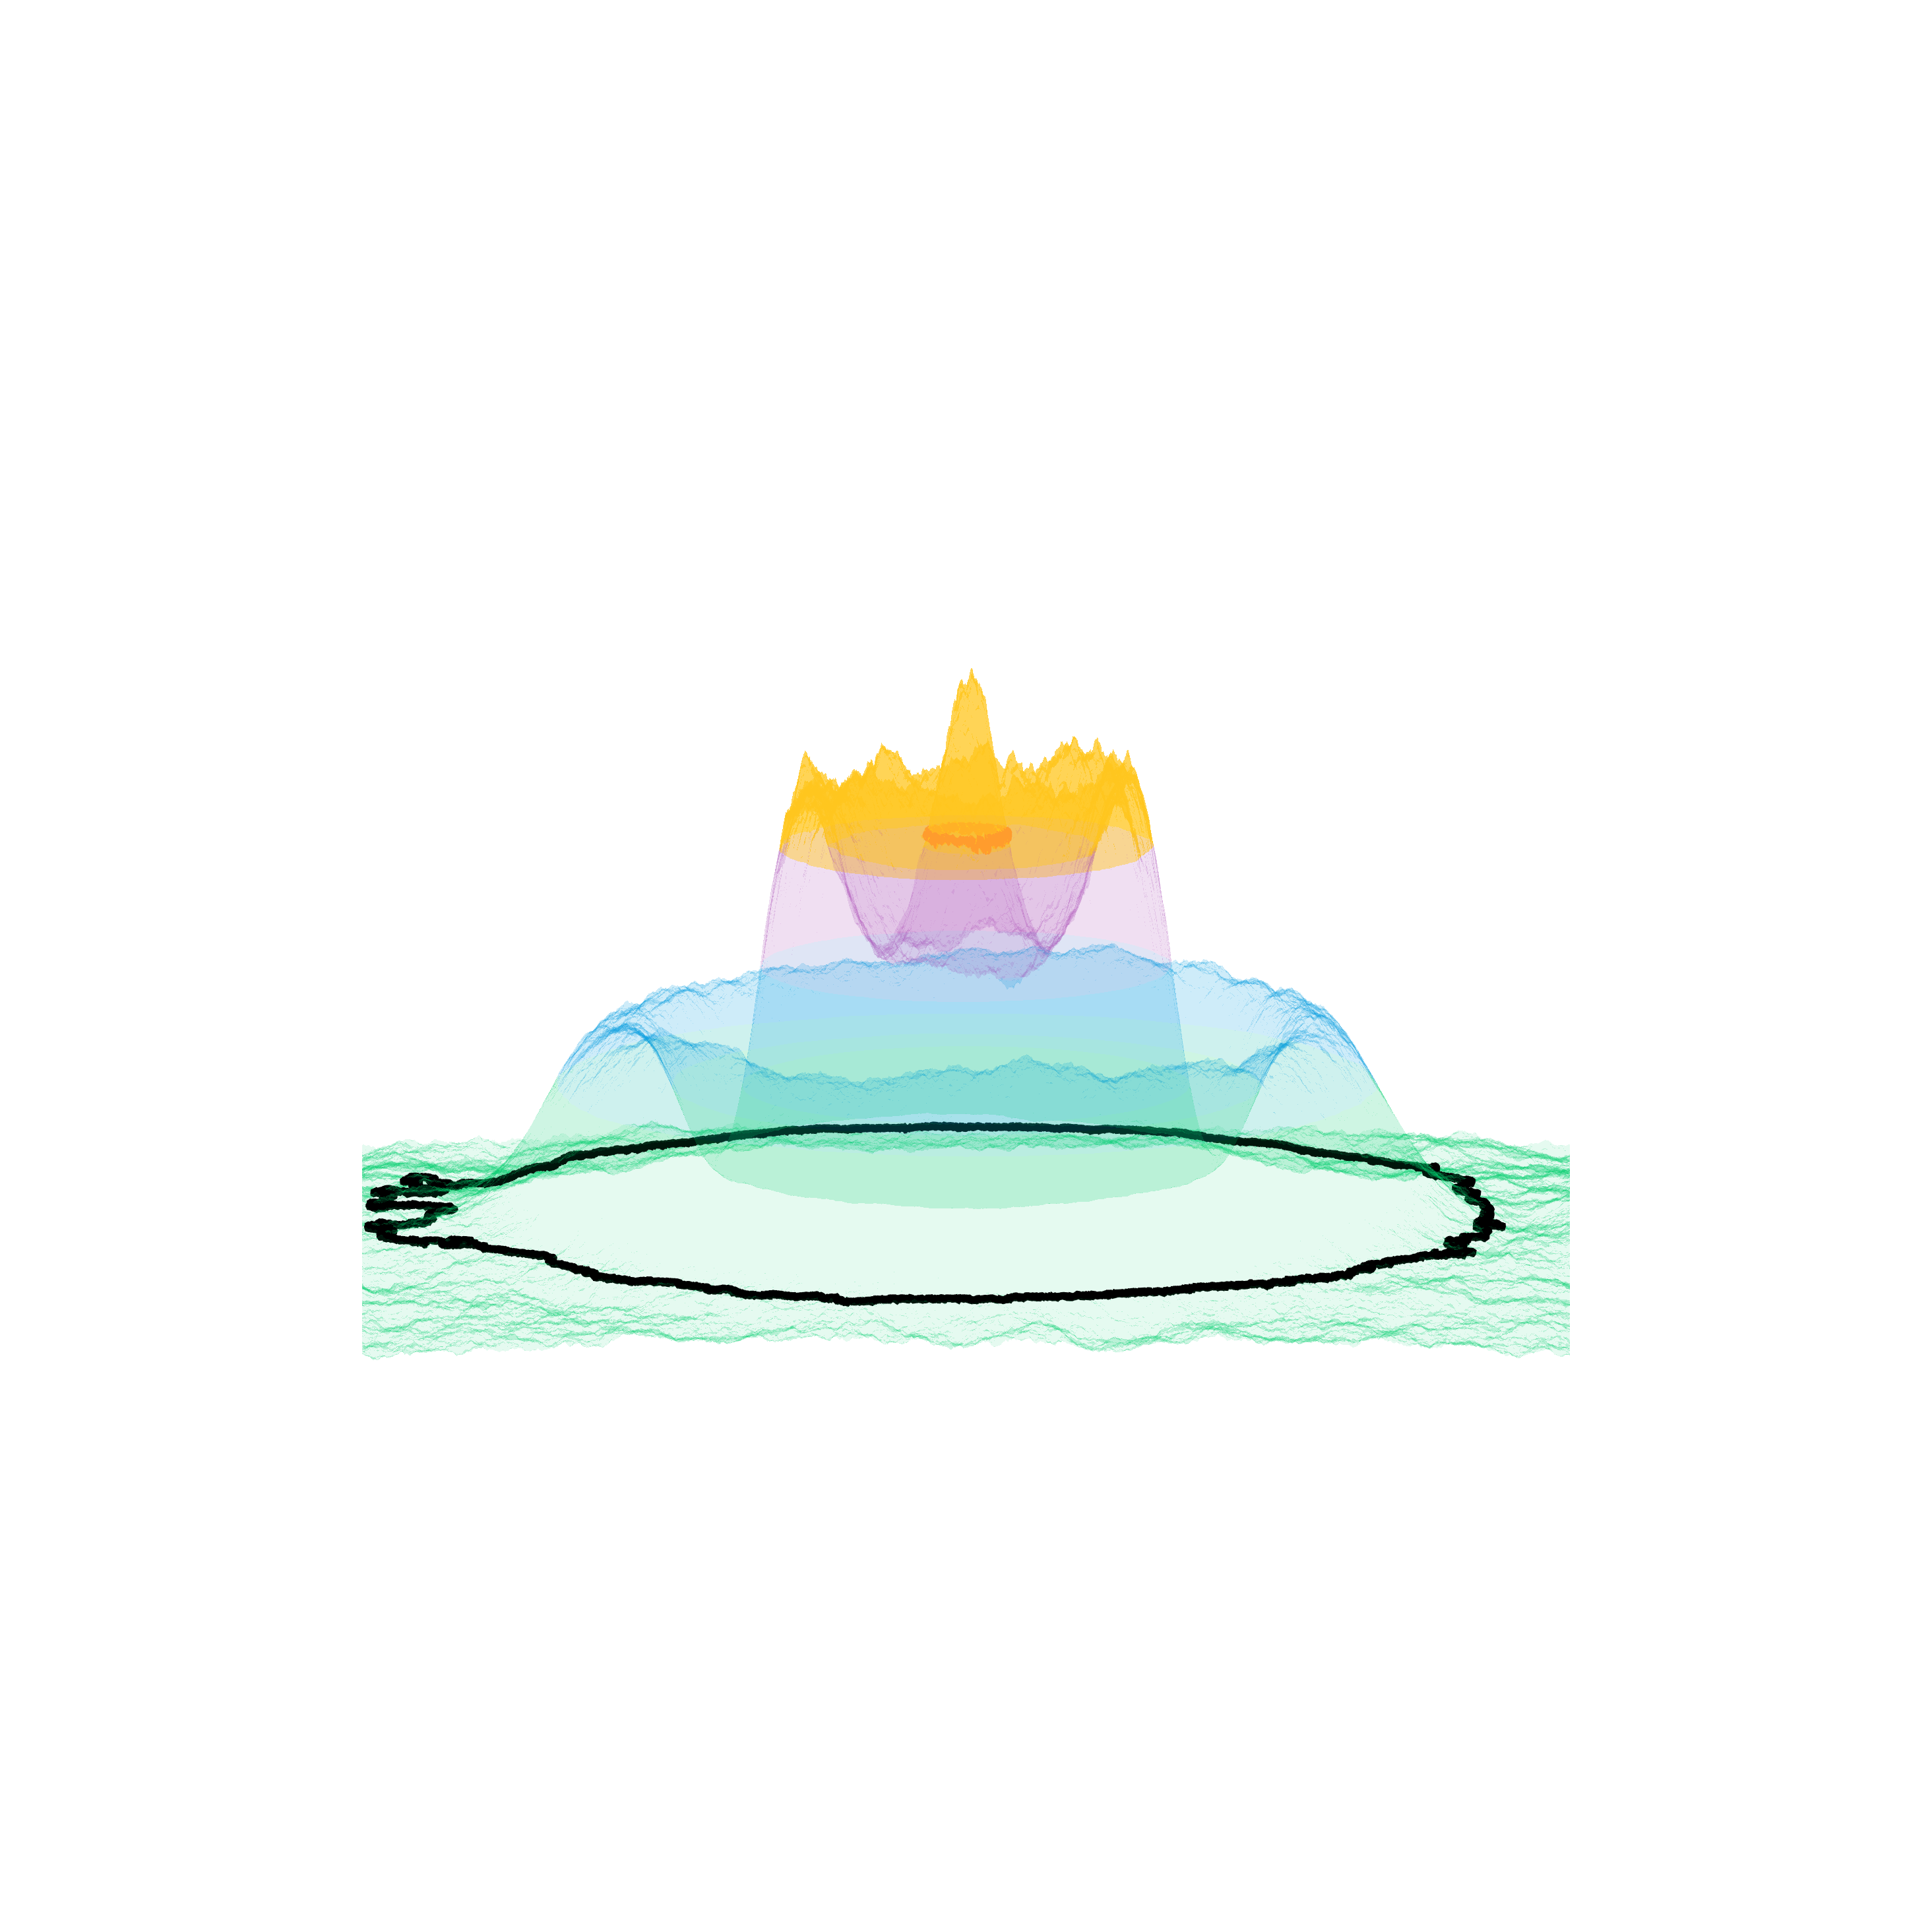
\includegraphics[trim=500 800 500 800, clip, width=0.24\textwidth]{figures/matching-surf_side-1_2.png}
  
\includegraphics[trim=500 500 500 500, clip, width=0.24\textwidth]{figures/matching-surf_top-1.png}
  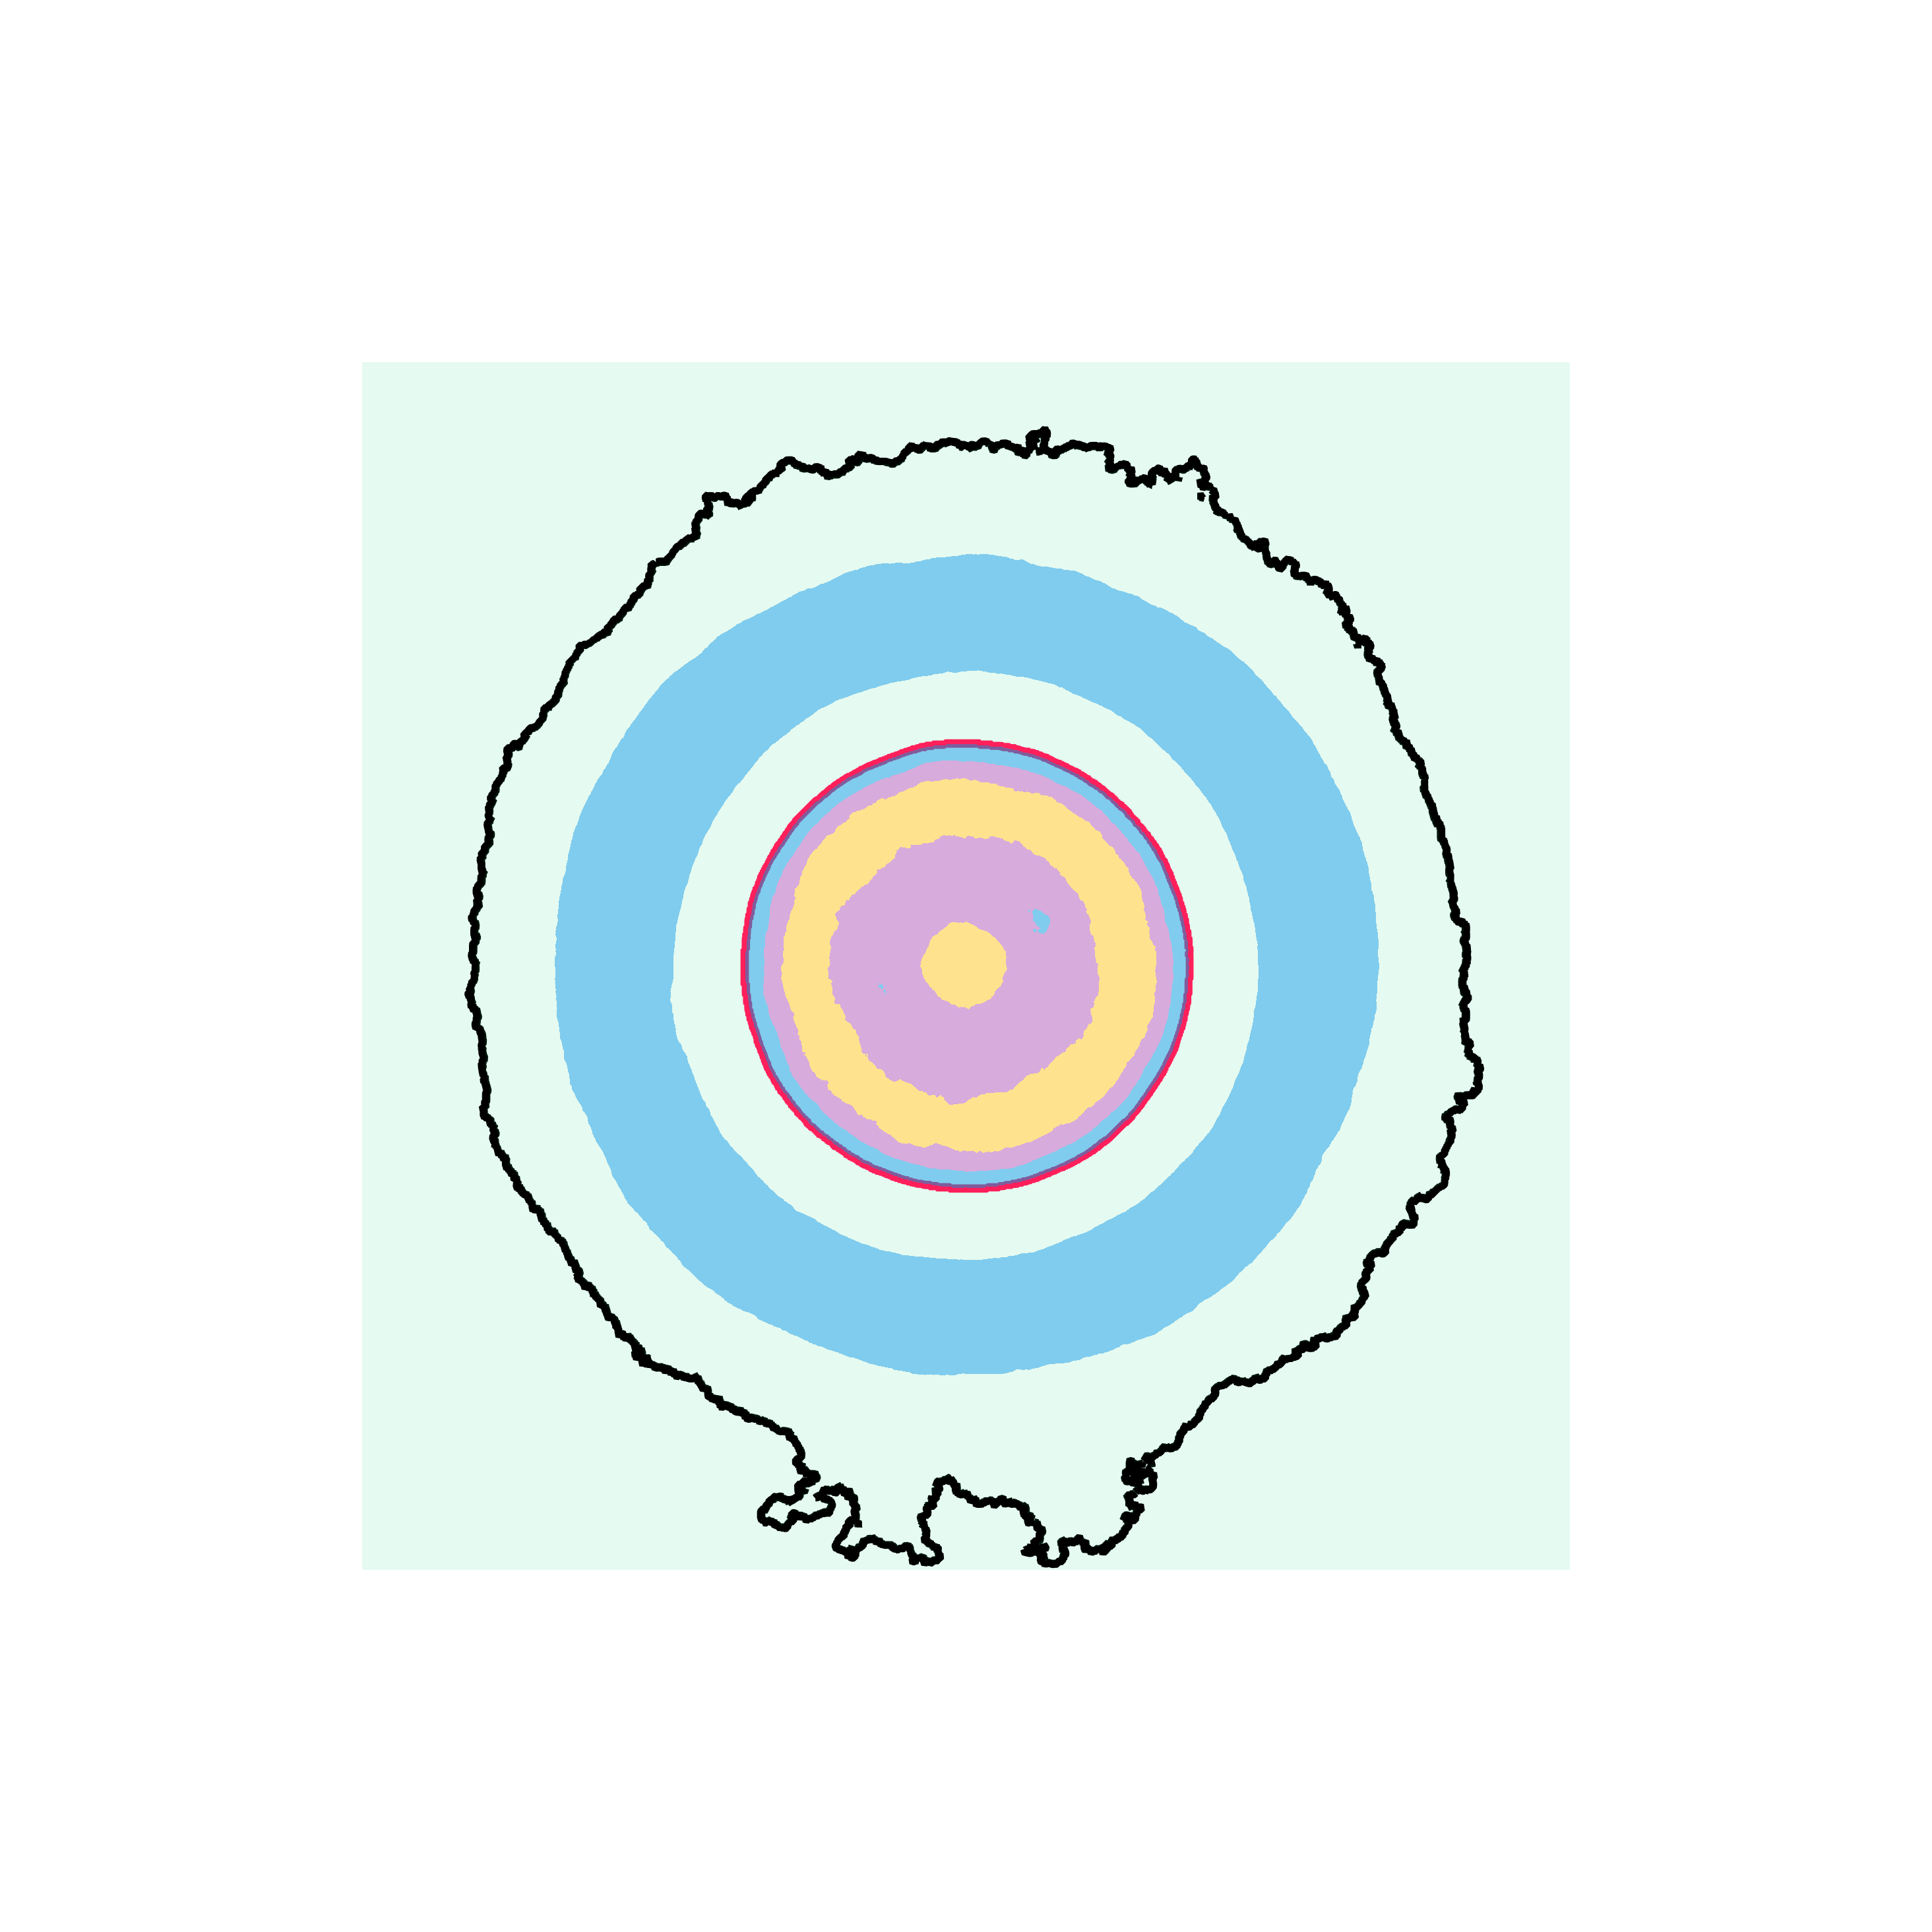
\includegraphics[trim=500 500 500 500, clip, width=0.24\textwidth]{figures/matching-surf_top-1_0.png}
  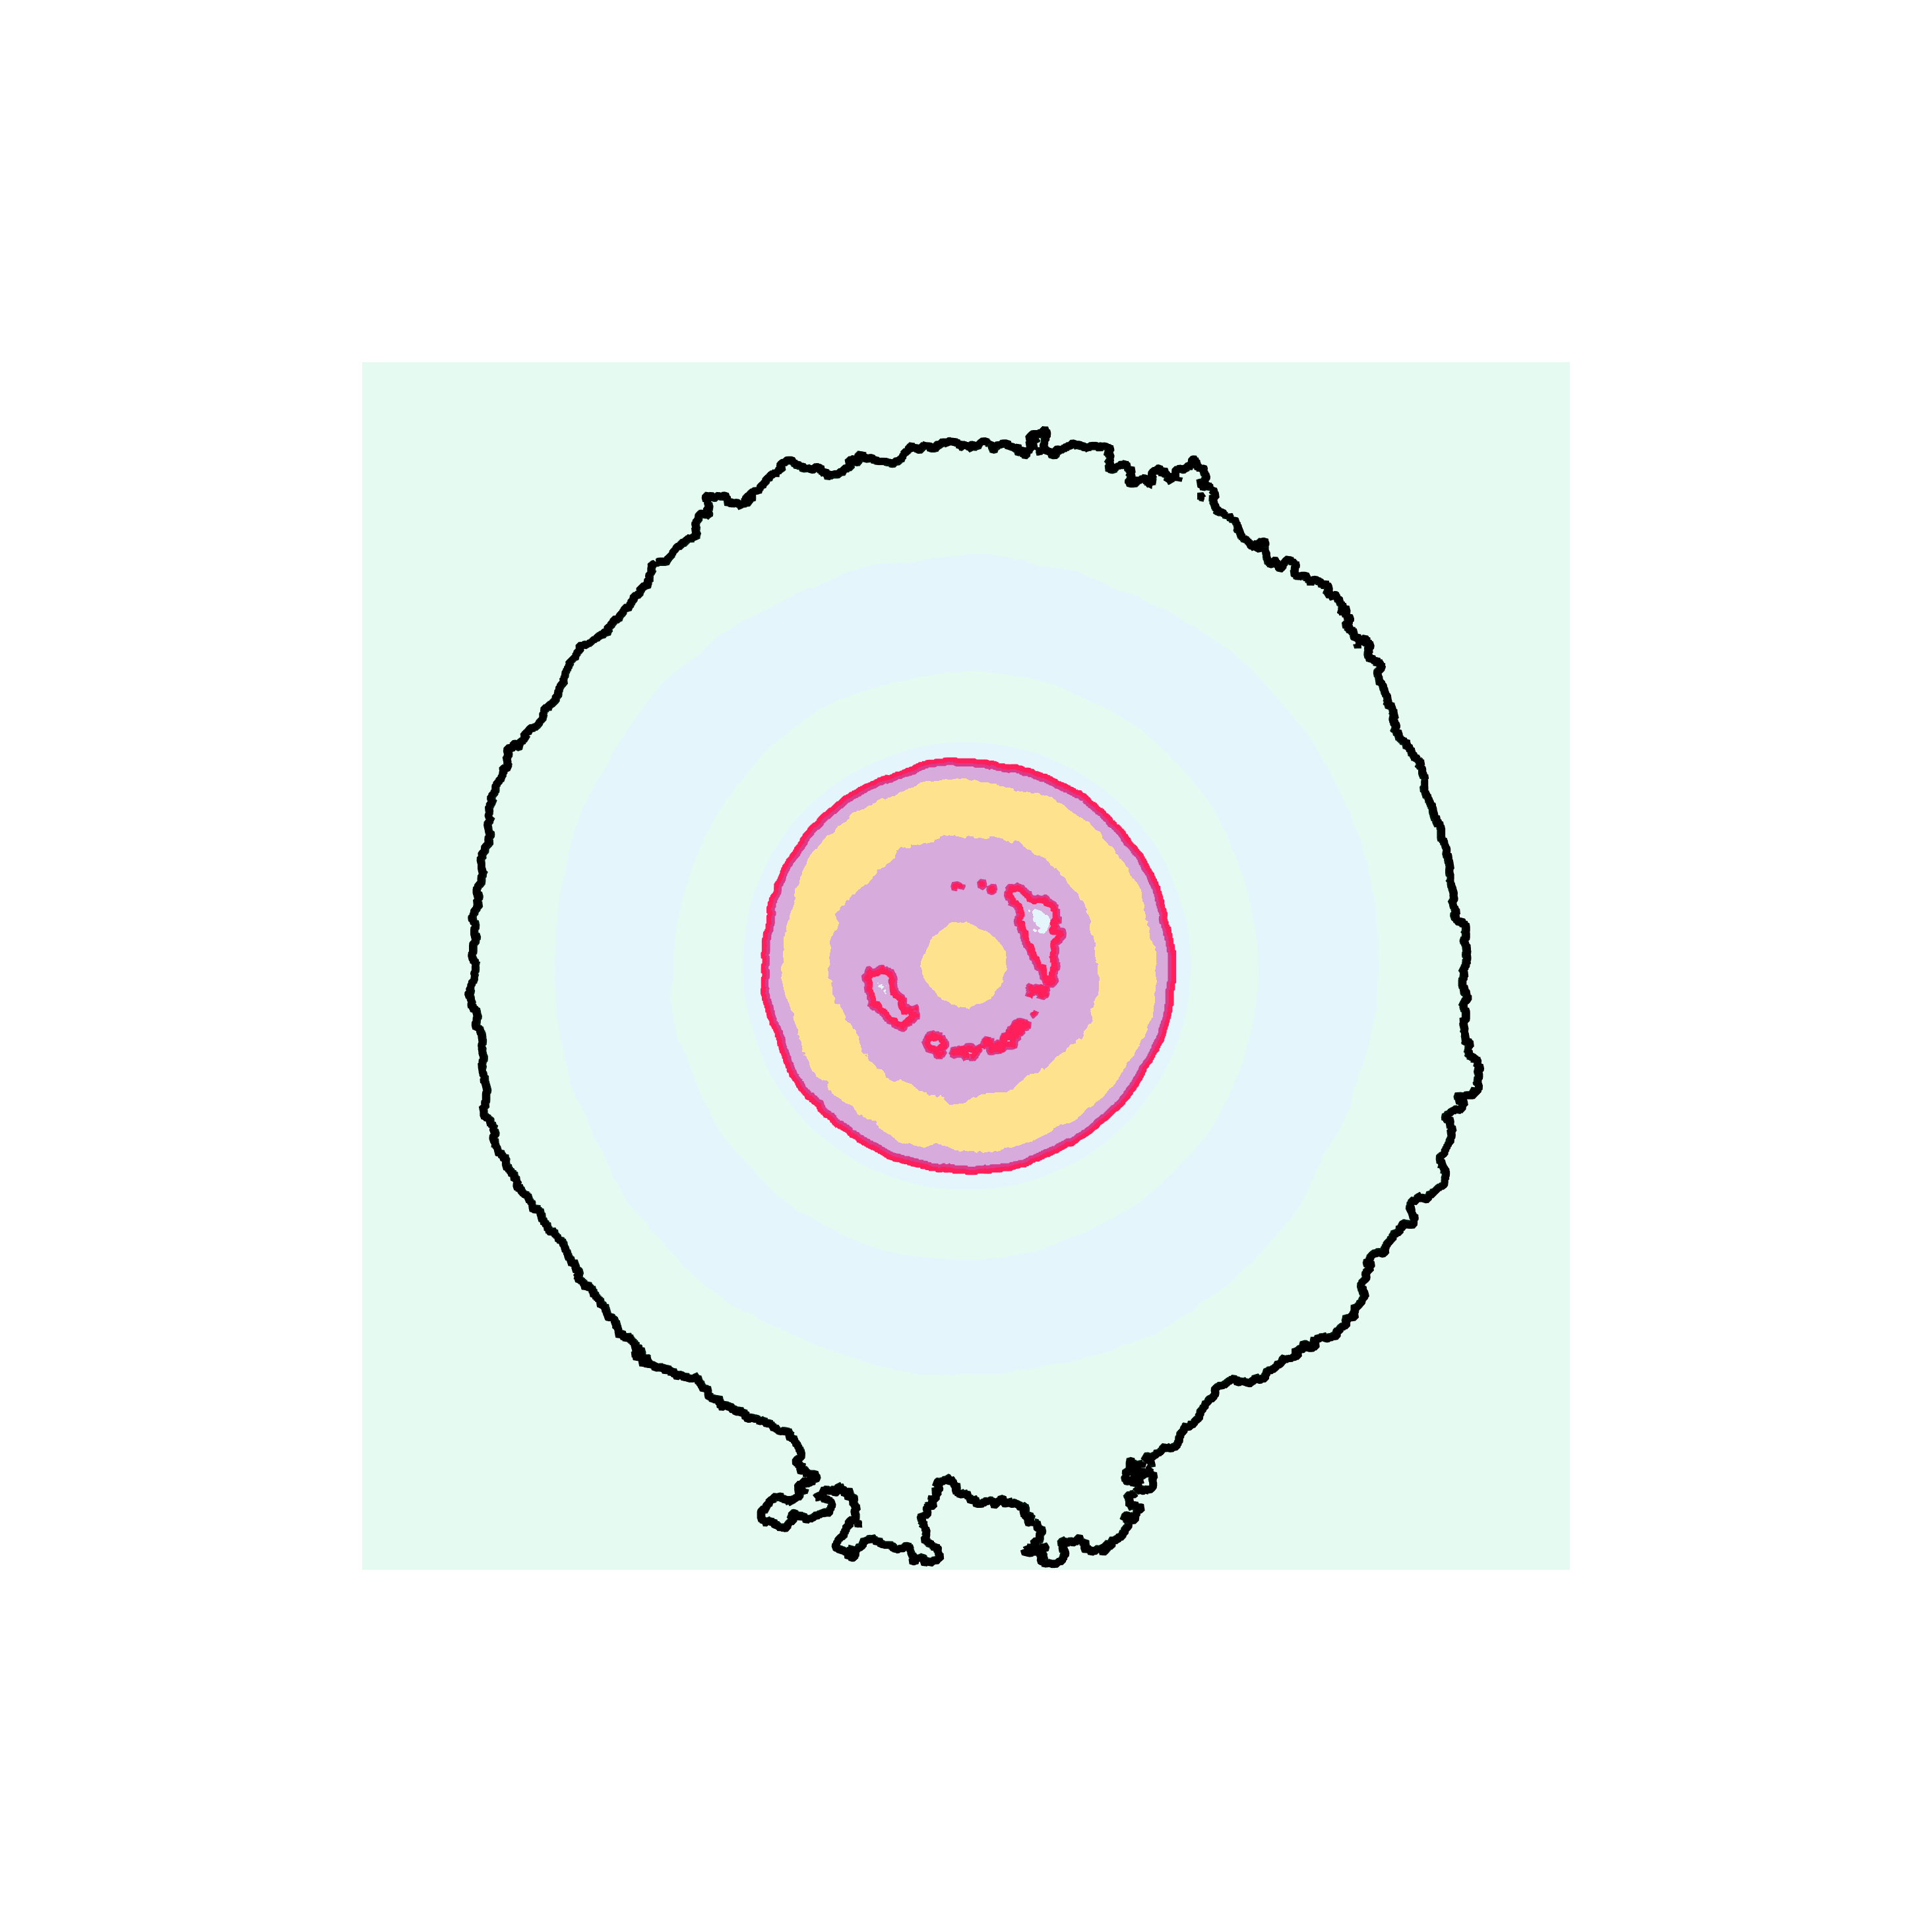
\includegraphics[trim=500 500 500 500, clip, width=0.24\textwidth]{figures/matching-surf_top-1_1.png}
  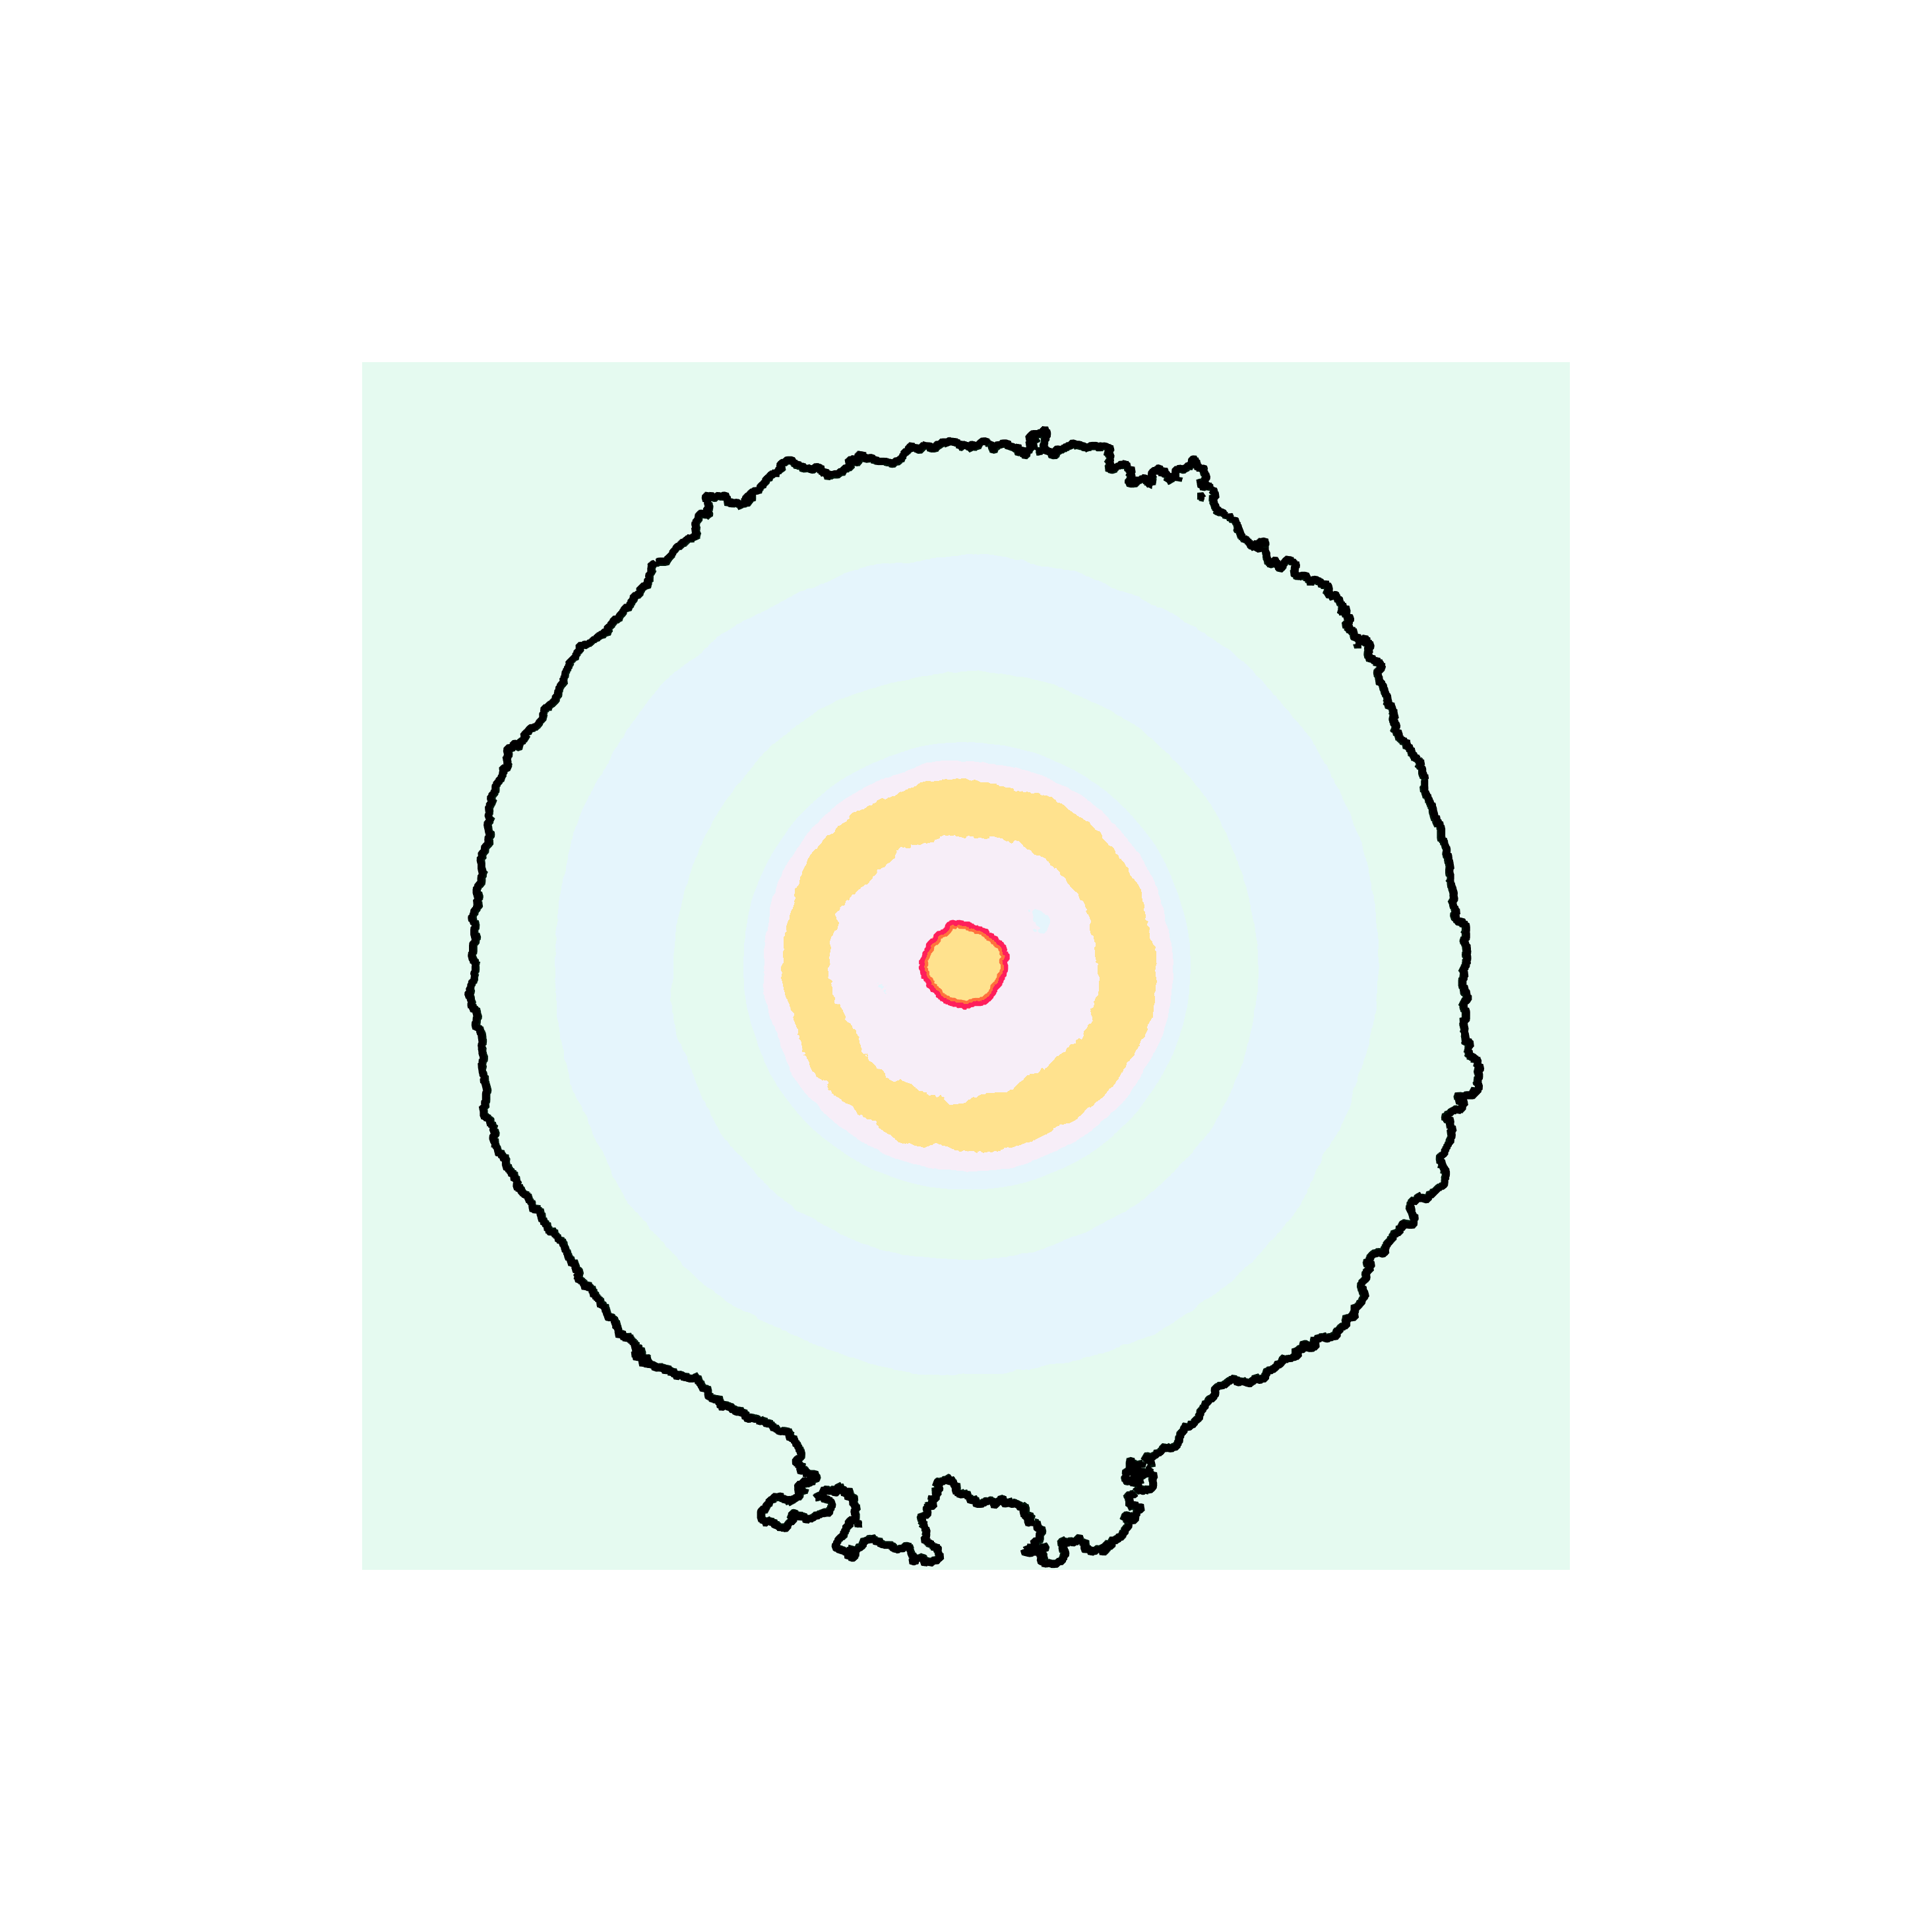
\includegraphics[trim=500 500 500 500, clip, width=0.24\textwidth]{figures/matching-surf_top-1_2.png}
  \caption{(Top) $\hom_1$ persistence diagrams of the function depicted in Figure~\ref{fig:ripple1} restricted to \emph{superlevel} sets at $\omega = 0.3, 0.5,$ and $0.7$ (on a $1024\times 1024$ grid).
  The matching is shown between a feature in the full diagram (marked with a diamond) with its representative cycle in black.
  The corresponding representative cycle in the restricted diagram is pictured in red.}\label{fig:restricted}
\end{figure}

Figure~\ref{fig:restricted} shows this distance for a feature that persists throughout the diagram.
As the restricted diagram in full resolution the restricted filtration is a subset of the full filtration, so these features can be matched by their death simplices.
For illustrative purposes we also show the representative cycles associated with these features.

We imagine a setting where we would like to classify a function using a sample that cannot be verified below some known $\omega$.
That is, we can only check for coverage of the superlevel set $D\setminus B_\omega$ using the variation of the TCC we have introduced in the previous sections.
We would then like to classify the function with the bottleneck distance to a set of known functions based on the region we cover.
However, as we have shown, the restricted diagram may contain artifacts of features born before $\omega$ which will skew our measurement.
Instead, as $\omega$ is known, we can compare the \emph{relative} diagram the collection of \emph{truncated} diagrams of known functions to get a better classification.

\paragraph*{Relative diagrams and reconstruction.}

\begin{figure}[htbp]
  \centering
  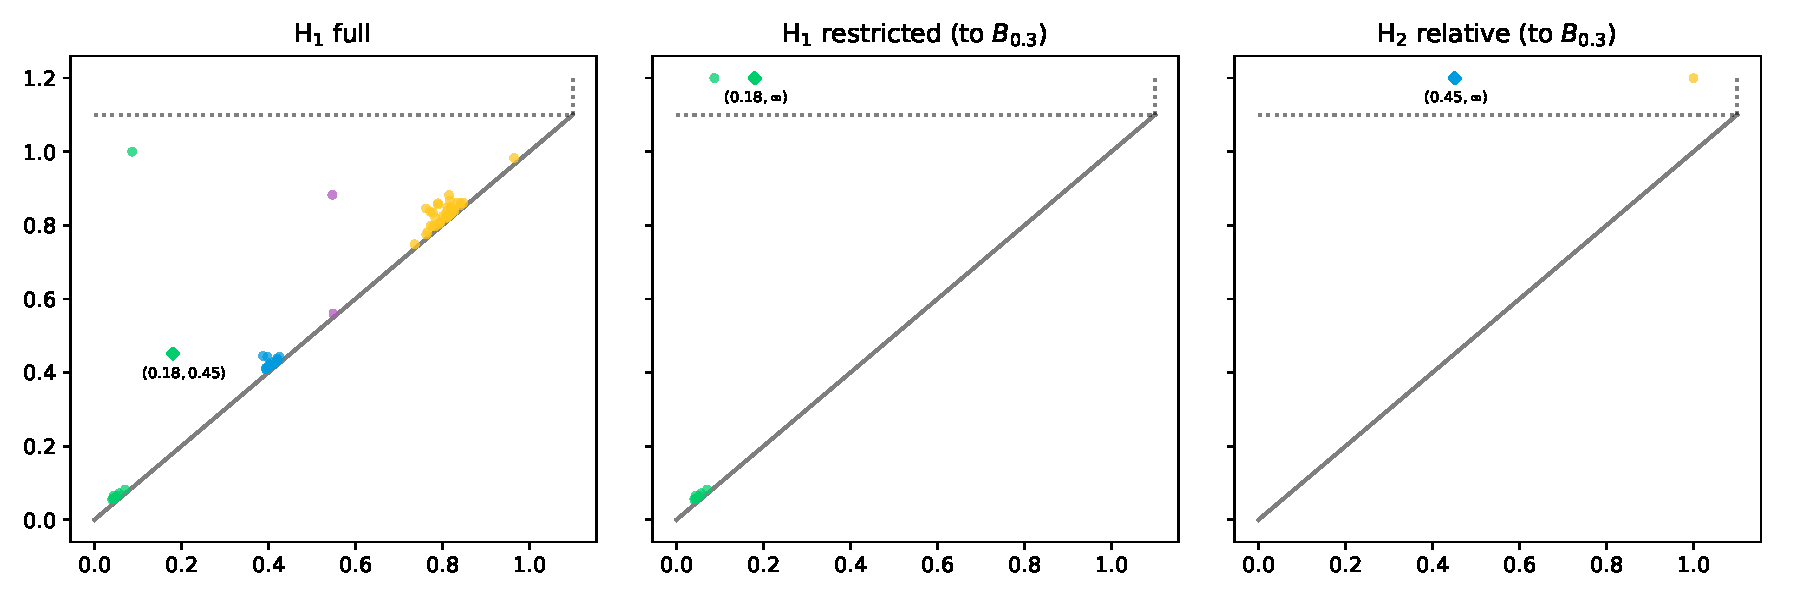
\includegraphics[width=0.9\textwidth]{figures/relative-dgm-0_0.pdf}
  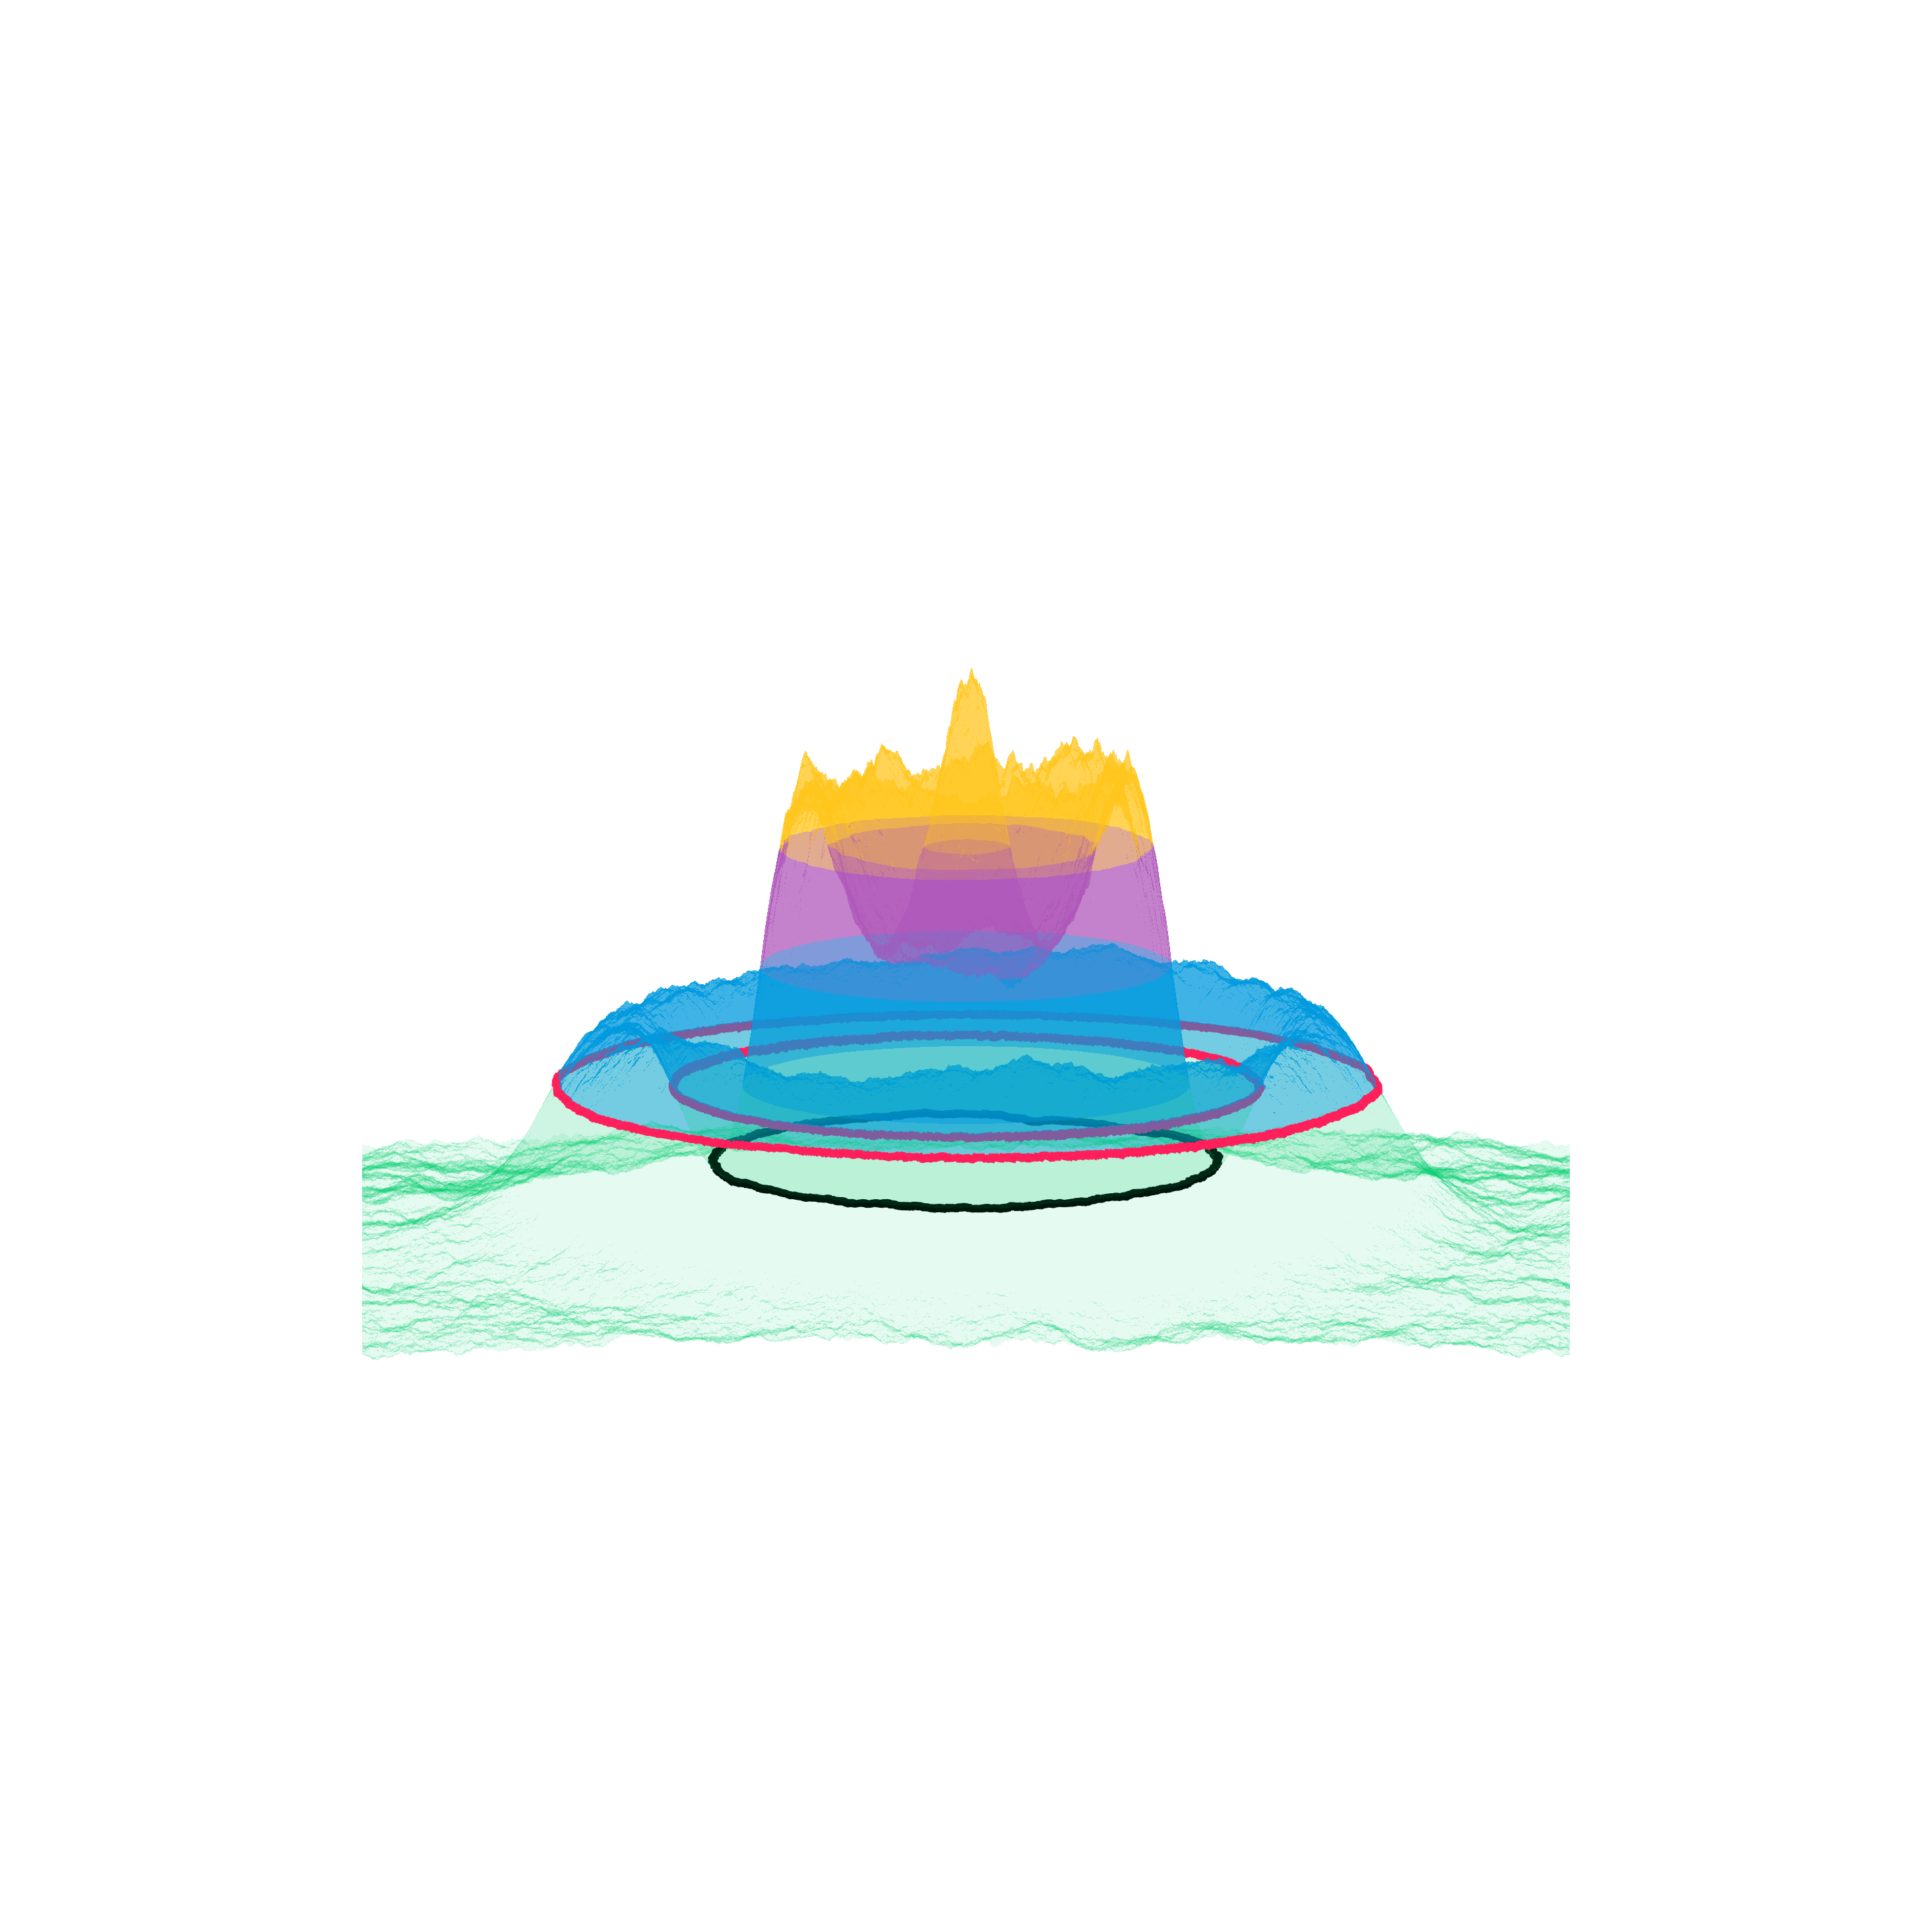
\includegraphics[trim=500 800 500 800, clip, width=0.35\textwidth]{figures/relative-surf_side-0_0.png}
  
\includegraphics[trim=500 500 500 500, clip, width=0.25\textwidth]{figures/relative-surf_top-0_0.png}
  % \caption{(Left) Full $\hom_1$ persistence diagram, (middle) $\hom_1$ persistence diagram of the function restricted to the \emph{sub}-levelset $B_{0.3}$, (right) $\hom_2$ persistence diagram of the the function realtive to the sub-levelset $B_{0.3}$.
  \caption{(Top) The indicated infinite features in the restricted and relative diagrams correspond to the birth and death of the 1-feature $(0.18, 0.45)$ in the full diagram.
  (Bottom) In black, the representative cycle of the infinite 1-feature born at 0.18 in the restricted diagram is shown in black.
  In red, the \emph{boundary} of the representative \emph{relative} 2-cycle born at 0.45 in the relative diagram is shown in red.}\label{fig:relative1}
\end{figure}

Now, imagine we obtain the persistence diagram of our sublevel set $B_\omega$.
That is, we now know that we cover $B_\omega$, or some subset, and do not want to re-compute the diagram above $\omega$.
If we compute the persistence diagram of the function restricted to the \emph{sublevel} set $B_\omega$ any 1-dimensional features born before $\omega$ that die after $\omega$ will remain infinite features in this restricted (below) diagram.
Indeed, we could match these infinite 1-features with the corresponding shifted finite 1-features in the restricted (above) diagram, as shown in Figure~\ref{fig:restricted}.
However, that would require sorting through all finite features that are born near $\omega$ and deciding if they are in fact features of the full diagram that have been shifted.

Recalling that these same features become infinite 2-features in the relative diagram, we can use the relative diagram instead and match infinite 1-features of the diagram restricted below to infinite 2-features in the relative diagram, as shown in Figures~\ref{fig:relative1} and~\ref{fig:relative2}.
For this example the sequence of birth times of relative 2-features in \emph{decreasing} order correspond to the deaths of restricted 1-features in \emph{increasing} order.
How to construct this matching in general, especially in the presence of infinite features in the full diagram, is the subject of future research.

\begin{figure}[htbp]
  \centering
  \includegraphics[width=0.9\textwidth]{figures/relative-dgm-0_1.pdf}
  \includegraphics[trim=500 800 500 800, clip, width=0.35\textwidth]{figures/relative-surf_side-0_1.png}
  \includegraphics[trim=500 500 500 500, clip, width=0.25\textwidth]{figures/relative-surf_top-0_1.png}
  \caption{The infinite 1-features of the restricted diagram can be matched with the infinite 2-features of the relative diagrams.
  The sequence of birth times of relative 2-features in \emph{decreasing} order correspond to the deaths of restricted 1-features in \emph{increasing} order.}\label{fig:relative2}
\end{figure}

  % \clearpage
  %
  % \section{Conclusions}
  % \input{trajectories}
  % \input{future}

  \bibliographystyle{unsrt}
  \bibliography{bibliography}
\end{document}
